% =============================================================================
%  ASSESSMENT OF RAILROAD BALLAST DEGRADATION UNDER MODIFIED DROP-WEIGHT
%  IMPACT LOADING CONDITIONS AND IMAGE-BASED MORPHOLOGICAL ANALYSIS
%
%  A B.Tech. Thesis - Gati Shakti Vishwavidyalaya, Vadodara
%  Authors: Durgesh Kumar Legha (2270007) & Sandeep Patel (2280043)
%  Supervisor: Dr. Dinesh Gundavaram
%
%  Compilation: pdflatex -> bibtex (optional) -> pdflatex -> pdflatex
% =============================================================================
\documentclass[12pt,a4paper,oneside]{report}

% -----------------------------------------------------------------------------
%  Page geometry & basic typography
% -----------------------------------------------------------------------------
\usepackage[a4paper,top=2.5cm,bottom=2.5cm,left=3.2cm,right=2.5cm,headheight=15pt]{geometry}
\usepackage[T1]{fontenc}
\usepackage[utf8]{inputenc}
\usepackage{lmodern}
\usepackage{textcomp}
\usepackage{microtype}
\usepackage{setspace}
\onehalfspacing

% -----------------------------------------------------------------------------
%  Maths, science, units
% -----------------------------------------------------------------------------
\usepackage{amsmath,amssymb,amsfonts}
\usepackage{mathtools}
\usepackage{siunitx}
\sisetup{
    detect-all,
    per-mode=symbol,
    inter-unit-product=\ensuremath{\,\cdot\,},
    range-phrase=--,
    range-units=single
}
\DeclareSIUnit\tonne{t}

% -----------------------------------------------------------------------------
%  Tables, figures, captions
% -----------------------------------------------------------------------------
\usepackage{graphicx}
\graphicspath{{figures/}}
\usepackage{float}
\usepackage{booktabs}
\usepackage{array}
\usepackage{tabularx}
\usepackage{longtable}
\usepackage{multirow}
\usepackage{multicol}
\usepackage{rotating}
\usepackage{adjustbox}
\usepackage{makecell}
\renewcommand{\arraystretch}{1.15}

\usepackage[font=small,labelfont=bf,format=plain,justification=centering,
            labelsep=period]{caption}
\usepackage{subcaption}

% -----------------------------------------------------------------------------
%  Cross-references, hyperlinks, bibliography
% -----------------------------------------------------------------------------
\usepackage[hidelinks,bookmarksopen,bookmarksopenlevel=1]{hyperref}
\hypersetup{
    colorlinks=false,
    pdftitle={Assessment of Railroad Ballast Degradation under Modified
              Drop-Weight Impact Loading Conditions and Image-Based
              Morphological Analysis},
    pdfauthor={Durgesh Kumar Legha and Sandeep Patel},
    pdfsubject={B.Tech. Thesis, Gati Shakti Vishwavidyalaya},
    pdfkeywords={ballast, drop-weight impact, 3D morphology, RDSO,
                 Indian Railways, fouling index}
}
\usepackage[noabbrev,capitalise]{cleveref}

% -----------------------------------------------------------------------------
%  Lists, headers, code, miscellaneous
% -----------------------------------------------------------------------------
\usepackage{enumitem}
\setlist{itemsep=2pt,topsep=4pt}
\usepackage{fancyhdr}
\pagestyle{fancy}
\fancyhf{}
\renewcommand{\headrulewidth}{0.4pt}
\fancyhead[L]{\nouppercase{\leftmark}}
\fancyhead[R]{\thepage}
\fancypagestyle{plain}{\fancyhf{}\fancyfoot[C]{\thepage}\renewcommand{\headrulewidth}{0pt}}

\usepackage{xcolor}
\definecolor{codebg}{HTML}{F7F7F7}
\definecolor{codekw}{HTML}{0033B3}
\definecolor{codestr}{HTML}{067D17}
\definecolor{codecom}{HTML}{8C8C8C}

\usepackage{listings}
\lstdefinestyle{pythonstyle}{
    language=Python,
    backgroundcolor=\color{codebg},
    basicstyle=\footnotesize\ttfamily,
    keywordstyle=\color{codekw}\bfseries,
    stringstyle=\color{codestr},
    commentstyle=\color{codecom}\itshape,
    numbers=left,
    numberstyle=\tiny\color{gray},
    numbersep=8pt,
    frame=single,
    framesep=4pt,
    breaklines=true,
    breakatwhitespace=true,
    showstringspaces=false,
    tabsize=4,
    captionpos=b
}
\lstset{style=pythonstyle}

\usepackage{titlesec}
\titleformat{\chapter}[display]
    {\normalfont\Huge\bfseries}
    {\chaptertitlename\ \thechapter}{18pt}{\Huge}
\titlespacing*{\chapter}{0pt}{-30pt}{20pt}

% -----------------------------------------------------------------------------
%  Convenience macros
% -----------------------------------------------------------------------------
\newcommand{\FIIN}{\ensuremath{\mathit{FI}_{\mathrm{IN}}}}
\newcommand{\PoneM}{\ensuremath{P_{0.075}}}
\newcommand{\PtwoM}{\ensuremath{P_{20}}}
\newcommand{\Ke}{\ensuremath{K_{e}}}
\newcommand{\Vch}{\ensuremath{V_{\mathrm{ch}}}}
\newcommand{\Ach}{\ensuremath{A_{\mathrm{ch}}}}
\newcommand{\Deq}{\ensuremath{D_{\mathrm{eq}}}}
\newcommand{\Ap}{\ensuremath{A_{p}}}
\newcommand{\Ab}{\ensuremath{A_{b}}}
\newcommand{\dmax}{\ensuremath{d_{\max}}}
\newcommand{\dV}{\ensuremath{\%\Delta V}}
\newcommand{\dPsi}{\ensuremath{\%\Delta\Psi}}
\newcommand{\dC}{\ensuremath{\%\Delta C}}
\newcommand{\DegC}{\ensuremath{^{\circ}\mathrm{C}}}

% -----------------------------------------------------------------------------
\title{Assessment of Railroad Ballast Degradation under Modified Drop-Weight
       Impact Loading Conditions and Image-Based Morphological Analysis}
\author{Durgesh Kumar Legha \and Sandeep Patel}
\date{April 2026}

% =============================================================================
\begin{document}

% ------------------------ FRONT MATTER ---------------------------------------
\pagenumbering{roman}

% =============================================================================
%  Title page (single-page, compact)
% =============================================================================
\begin{titlepage}
\centering
\thispagestyle{empty}
\setlength{\parskip}{0pt}

% Decorative top double rule
{\color{gsvblue}\rule{\textwidth}{1pt}}\\[1pt]
{\color{gsvblue}\rule{\textwidth}{0.3pt}}

\vspace{0.25cm}
{\small\itshape\color{gsvblue}A B.Tech.\ Thesis in Civil Engineering
\;|\; Specialisation: Rail Engineering}

\vspace{0.45cm}
{\large\bfseries\color{gsvblue}%
ASSESSMENT OF RAILROAD BALLAST DEGRADATION\\[2pt]
UNDER MODIFIED DROP-WEIGHT IMPACT LOADING\\[2pt]
CONDITIONS AND IMAGE-BASED MORPHOLOGICAL ANALYSIS\par}

\vspace{0.35cm}
{\color{gsvaccent}\rule{0.4\textwidth}{0.6pt}}

\vspace{0.3cm}
{\small\itshape submitted by}

\vspace{0.2cm}
{\large\bfseries DURGESH KUMAR LEGHA}\\[1pt]
{\small (Roll No.\ 2270007)}\\[5pt]
{\large\bfseries SANDEEP PATEL}\\[1pt]
{\small (Roll No.\ 2280043)}

\vspace{0.3cm}
{\small\itshape under the supervision of}

\vspace{0.15cm}
{\large\bfseries Dr.\ Dinesh Gundavaram}\\[1pt]
{\footnotesize Assistant Professor, School of Civil Engineering}

\vspace{0.35cm}
{\small In Partial Fulfilment of the Requirements for the Degree of\par}
\vspace{2pt}
{\normalsize\bfseries Bachelor of Technology in Civil Engineering\par}

\vspace{0.4cm}

\includegraphics[height=3.2cm]{image1.png}

\vspace{0.25cm}
{\Large\bfseries\color{gsvblue} Gati Shakti Vishwavidyalaya\par}
\vspace{2pt}
{\footnotesize\itshape A Central University under the Ministry of Railways,
Government of India\par}
{\footnotesize Lalbaug, Vadodara 390004, Gujarat, India\par}

\vfill
{\large\bfseries\color{gsvblue} April 2026\par}

\vspace{0.2cm}
{\color{gsvblue}\rule{\textwidth}{0.3pt}}\\[1pt]
{\color{gsvblue}\rule{\textwidth}{1pt}}
\end{titlepage}

% =============================================================================
%  Candidate's declaration, supervisor's certificate, approval certificate
% =============================================================================
\chapter*{Candidate's Declaration}
\addcontentsline{toc}{chapter}{Candidate's Declaration}
\thispagestyle{plain}

We hereby certify that
\begin{enumerate}[label=(\roman*)]
    \item The work contained in this thesis is original and has been carried
          out by us jointly under the guidance of our supervisor,
          Dr.\ Dinesh Gundavaram, Gati Shakti Vishwavidyalaya, Vadodara.
    \item The work has not been submitted in whole or in part to any other
          institute or university for the award of any degree, diploma, or
          certificate.
    \item We have followed the academic guidelines and ethical code of
          conduct provided by Gati Shakti Vishwavidyalaya in preparing this
          thesis.
    \item Wherever we have used materials (data, experimental results,
          theoretical analyses, figures, tables, or text) from other sources,
          we have given due credit to them by citing them in the text of the
          thesis and by giving full bibliographic details in the reference
          list. Where required, permission from the copyright owners has been
          obtained.
    \item The experimental programme reported in this thesis was conducted by
          both candidates jointly at Gati Shakti Vishwavidyalaya.
\end{enumerate}

\vspace{2cm}

\noindent\begin{minipage}[t]{0.45\textwidth}
\centering
\rule{6cm}{0.4pt}\\[2pt]
\textbf{Durgesh Kumar Legha}\\
(2270007)
\end{minipage}\hfill
\begin{minipage}[t]{0.45\textwidth}
\centering
\rule{6cm}{0.4pt}\\[2pt]
\textbf{Sandeep Patel}\\
(2280043)
\end{minipage}

% -----------------------------------------------------------------------------
\chapter*{Certificate of Thesis Supervisor}
\addcontentsline{toc}{chapter}{Certificate of Thesis Supervisor}
\thispagestyle{plain}

This is to certify that the thesis entitled
\textit{``Assessment of Railroad Ballast Degradation under Modified
Drop-Weight Impact Loading Conditions and Image-Based Morphological
Analysis''}, submitted by Durgesh Kumar Legha (Roll No.\ 2270007) and
Sandeep Patel (Roll No.\ 2280043) to Gati Shakti Vishwavidyalaya, is a record
of bonafide research work carried out jointly by them under my supervision.
The work embodied in this thesis has not been submitted, in whole or in part,
for the award of any degree, diploma, or certificate at any other institute
or university. In my opinion, this thesis is of the standard required for the
degree of Bachelor of Technology in Civil Engineering (Specialisation:
Railway Engineering), and I consider it worthy of consideration for the said
degree.

\vspace{2.0cm}
\noindent\rule{7cm}{0.4pt}\\[2pt]
\textbf{Dr.\ Dinesh Gundavaram}\\
Thesis Supervisor\\
Assistant Professor\\
School of Civil Engineering,\\
Gati Shakti Vishwavidyalaya,\\
Vadodara, Gujarat -- 390004.

\vspace{1.0cm}
\noindent Date: \rule{4cm}{0.4pt}\\
Place: Vadodara

% -----------------------------------------------------------------------------
\chapter*{Certificate of Approval}
\addcontentsline{toc}{chapter}{Certificate of Approval}
\thispagestyle{plain}

Certified that the thesis entitled
\textit{``Assessment of Railroad Ballast Degradation under Modified
Drop-Weight Impact Loading Conditions and Image-Based Morphological
Analysis''} submitted by Durgesh Kumar Legha (Roll No.\ 2270007) and
Sandeep Patel (Roll No.\ 2280043) to Gati Shakti Vishwavidyalaya for the
award of the Degree of Bachelor of Technology in Civil Engineering
(Specialisation: Railway Engineering) has been accepted by the B.\,Tech.\
project committee members. The project presentation by the candidates was
held on 23\textsuperscript{rd} April 2026.

\vspace{2.0cm}
\noindent\begin{minipage}[t]{0.45\textwidth}
\centering
\rule{6cm}{0.4pt}\\[2pt]
\textbf{Dr.\ Dinesh Gundavaram}\\
Thesis Supervisor and \\
B.\,Tech.\ Project Coordinator
\end{minipage}\hfill
\begin{minipage}[t]{0.45\textwidth}
\centering
\rule{6cm}{0.4pt}\\[2pt]
\textbf{Dr.\ Dinesh Gundavaram}\\
B.\,Tech.\ Project Coordinator
\end{minipage}

\vspace{1.5cm}
\noindent\begin{center}
\rule{6cm}{0.4pt}\\[2pt]
\textbf{Dr.\ Pradeep}\\
B.\,Tech.\ Programme Coordinator
\end{center}

% =============================================================================
%  Acknowledgements
% =============================================================================
\chapter*{Acknowledgement}
\addcontentsline{toc}{chapter}{Acknowledgement}
\thispagestyle{plain}

We wish to place on record our deep sense of gratitude to all those without
whose guidance, encouragement, and support this work would not have reached
its present form.

Our foremost and most profound thanks are due to our supervisor,
Dr.\ Dinesh Gundavaram, Assistant Professor at Gati Shakti Vishwavidyalaya.
Across every stage of this project---from the first conversation about the
limitations of the conventional Aggregate Impact Value test, through the
careful re-conception of the large-scale drop-weight apparatus, the design of
the nine-configuration factorial matrix, the painstaking three-dimensional
scanning work, and finally the writing of this thesis---he has been a
patient and rigorous mentor. The intellectual standards he holds and the
clarity with which he insisted on first-principles reasoning are reflected in
every chapter that follows. Any errors or shortcomings that remain are our
own.

We express our sincere gratitude to the Hon'ble Vice Chancellor of Gati
Shakti Vishwavidyalaya for fostering an academic environment that encourages
research, innovation, and critical thinking. We are also thankful to the
Programme Coordinator and all faculty members for their structured guidance,
timely reviews, and valuable feedback, which helped keep this work on track.

We extend our appreciation to the laboratory technicians and technical staff
of Gati Shakti Vishwavidyalaya for their assistance and cooperation during
the experimental phases of this project. We also acknowledge the support
extended by other departments and faculty members whose indirect
contributions and institutional support facilitated the smooth execution of
this work.

On a personal note, we thank our families whose belief in the value of this
work was never conditional on the stage of its results, and our batchmates
in the Civil Engineering programme, whose conversations sharpened many of
the mechanistic interpretations that appear in the discussion chapter. In
particular we are grateful to the friends who kept us company through late
laboratory evenings on more occasions than we care to count.

Finally, we acknowledge the broader community of railway geotechnics
researchers whose published work we have cited in this thesis. The scientific
literature is a cumulative enterprise, and every modest contribution in this
document rests on decades of careful experimentation and thought by others.

\vspace{1.2cm}
\hfill\textbf{Durgesh \& Sandeep}\hspace{2cm}\mbox{}

% =============================================================================
%  Abstract
% =============================================================================
\chapter*{Abstract}
\addcontentsline{toc}{chapter}{Abstract}
\thispagestyle{plain}

The thesis focuses on addressing the critical issue of railway ballast
degradation, which significantly impacts the safety, stability, and
operational efficiency of railway tracks. Tailored specifically to the
unique conditions of Indian Railways, this research aims to develop a
deeper understanding of ballast behaviour under impact loading and to
predict the quantum of ballast degradation using 3D image processing as well
as machine-learning models.

At the core of the study is the modification of the European-standard
drop-weight impact test apparatus to better align with Indian railway
ballast specifications and operational conditions. The modified setup
accurately replicates on-field stress conditions experienced by ballast in
the Indian context, providing a more relevant and reliable framework for
analysis. The modified apparatus serves as a critical tool for evaluating
ballast degradation under controlled yet realistic conditions, delivering
nominal contact stresses of \SI{275}{\kilo\pascal} (at a \SI{300}{\milli\metre}
drop height) and \SI{523}{\kilo\pascal} (at a \SI{450}{\milli\metre} drop
height) corresponding to the \num{22.5}-tonne axle load characteristic of
Indian Railways.

A significant innovation in this study is the use of advanced 3D image
processing techniques to evaluate morphological changes in ballast particles
before and after impact testing. High-resolution 3D meshes are captured to
analyse changes in particle shape, size, and texture, providing a detailed
and quantitative understanding of ballast degradation. A paired-particle
protocol applied to 45 marked tracer particles across nine experimental
configurations enables precise measurement of deterioration, allowing
identification of critical thresholds and damage modes (diffuse abrasion vs.\
catastrophic fracture) that are not detectable through traditional sieve
analysis.

The outcomes of this study contribute to railroad ballast degradation
assessment using image-based morphology and machine learning, delivering a
scalable and accurate alternative to conventional physical testing, with
substantial implications for railway safety and maintenance planning.

\vspace{0.4cm}
\noindent\textbf{Keywords:} Railway ballast; drop-weight impact loading; RDSO
gradation; Fouling Index; 3D structured-light scanning; particle morphology;
under-ballast mats; ballast degradation.

% =============================================================================
%  Dedication + Outcomes of the project (Journals / Patents / Conferences)
% =============================================================================

% ---------- Dedication ----------
\cleardoublepage
\thispagestyle{empty}
\vspace*{4cm}
\begin{center}
{\Large\itshape\color{gsvblue} Dedicated to}\\[0.6cm]
{\large our families,}\\[0.2cm]
{\large our supervisor, and}\\[0.2cm]
{\large the engineers and operators of Indian Railways,}\\[0.6cm]
{\large whose patience and trust made this work possible.}
\end{center}
\vspace*{\fill}

% ---------- Outcomes ----------
\cleardoublepage
\chapter*{Outcomes of This Project}
\addcontentsline{toc}{chapter}{Outcomes of This Project}
\thispagestyle{plain}
\markboth{Outcomes of This Project}{}

\section*{\textcolor{gsvblue}{Journal Manuscripts}}
\begin{enumerate}[leftmargin=*,itemsep=4pt]
    \item Legha~D. and Gundavaram~D.,
          \emph{Composite Railway Sleepers: A Review of Mechanical
          Performance, Durability and Adoption Challenges},
          \textit{Railway Engineering Science} (2026)
          \textbf{(Under Review)}. (IF = 5.4)
    \item Legha~Durgesh~K., Gundavaram~Dinesh, Patel~Sandeep,
          \emph{A large-scale drop-weight impact testing apparatus for
          assessment of Indian Railway ballast: influence of stress level
          and subgrade--interlayer configuration on settlement and
          particle degradation},
          \textit{Construction and Building Materials} (2026)
          \textbf{(Under Review)}. (IF = 7.2)
\end{enumerate}

\section*{\textcolor{gsvblue}{Patents}}
\begin{enumerate}[leftmargin=*,itemsep=4pt]
    \item Gundavaram~D., Legha~D., (2026),
          \emph{Assessment of Railroad Ballast Degradation under Modified
          Drop-Weight Impact Loading Conditions.}
          (Indian Utility Patent) \textbf{(Draft Prepared)}.
\end{enumerate}

\section*{\textcolor{gsvblue}{Conference Papers}}
\begin{enumerate}[leftmargin=*,itemsep=4pt]
    \item Legha~D.K., Patel~S., Gundavaram~D., (2026)
          \emph{Optimization of Bitumen Content in Bitumen-Stabilized
          Ballast Using Flowability Characteristics},
          Recent Research on Environmental Earth Sciences, MedGU~2025,
          Springer. \textbf{(Accepted, In Press)}.
    \item Legha~D., Gundavaram~D., Mishra~G., (2026)
          \emph{Global Practices of Railway Drainage Systems with
          Emphasis on India and Emerging Innovation},
          Geotechnical Practices for Innovations and Sustainability,
          Proceedings of the Indian Geotechnical Conference (IGC~2025),
          Lecture Notes in Civil Engineering, Springer.
          \textbf{(Accepted, In Press)}.
\end{enumerate}

\vspace{0.6cm}
\begin{center}
\fbox{\parbox{0.8\textwidth}{
\centering\small
\textbf{\textcolor{gsvblue}{Scan the QR code for the project video}}\\[6pt]

\includegraphics[width=0.22\textwidth]{image3.png}\\[4pt]
\footnotesize\itshape
A short documentary of the apparatus design, test campaign, and analysis
pipeline.
}}
\end{center}


% Table of contents, list of figures/tables, abbreviations & symbols
\cleardoublepage\pdfbookmark[0]{Table of Contents}{toc}
\tableofcontents
\cleardoublepage\listoffigures
\cleardoublepage\listoftables
% =============================================================================
%  List of Abbreviations + Glossary of Terms (both auto-generated)
% =============================================================================
\clearpage
\markboth{List of Abbreviations}{}
\glsaddall
\printglossary[type=\acronymtype,style=long,nogroupskip,
               title={List of Abbreviations}]
\addcontentsline{toc}{chapter}{List of Abbreviations}

\clearpage
\markboth{Glossary of Terms}{}
\printglossary[type=main,style=altlist,nogroupskip,
               title={Glossary of Terms}]
\addcontentsline{toc}{chapter}{Glossary of Terms}

% =============================================================================
%  List of Symbols
% =============================================================================
\cleardoublepage
\chapter*{List of Symbols}
\addcontentsline{toc}{chapter}{List of Symbols}
\thispagestyle{plain}
\markboth{List of Symbols}{}

\begin{longtable}{@{}p{0.22\textwidth}p{0.72\textwidth}@{}}
    \toprule
    \textbf{Symbol} & \textbf{Meaning (units)}\\
    \midrule
    \endfirsthead
    \toprule
    \textbf{Symbol} & \textbf{Meaning (units)}\\
    \midrule
    \endhead
    \bottomrule
    \endlastfoot
    $A$           & Surface area of a particle (\si{\milli\metre\squared})\\
    $\Ach$        & Convex-hull surface area (\si{\milli\metre\squared})\\
    $a,b,c$       & Semi-axes of best-fit ellipsoid (\si{\milli\metre}),
                    $a\ge b\ge c$\\
    $C$           & Convexity $= V/\Vch$ (dimensionless)\\
    $D$           & Mould internal diameter (\si{\milli\metre})\\
    $\Deq$        & Equivalent spherical diameter
                    $=\left(6V/\pi\right)^{1/3}$ (\si{\milli\metre})\\
    $\dmax$       & Maximum particle size in a gradation (\si{\milli\metre})\\
    $E$           & Elongation $= I/L$ (dimensionless)\\
    $F$           & Flatness $= S/I$ (dimensionless)\\
    $g$           & Gravitational acceleration,
                    \SI{9.81}{\metre\per\second\squared}\\
    $h$           & Drop height of hammer
                    (\si{\milli\metre} or \si{\metre})\\
    $I$           & Intermediate bounding-box dimension (\si{\milli\metre})\\
    $\Ke$         & Kinetic energy of hammer at impact $= mgh$
                    (\si{\joule})\\
    $L$           & Long bounding-box dimension (\si{\milli\metre})\\
    $L/S$         & Aspect ratio (dimensionless)\\
    $(L+I)/(2S)$  & Flatness index (dimensionless)\\
    $m$           & Hammer mass (\si{\kilogram})\\
    $N$           & Number of blows (dimensionless)\\
    $n$           & Sample size (dimensionless)\\
    $p$           & Statistical $p$-value (dimensionless)\\
    $R$           & Roundness descriptor (dimensionless, scanner-specific)\\
    $S$           & Short bounding-box dimension (\si{\milli\metre})\\
    $t$           & Student's $t$-statistic (dimensionless)\\
    $V$           & Volume of a particle (\si{\milli\metre\cubed})\\
    $\Vch$        & Convex-hull volume (\si{\milli\metre\cubed})\\
    $\sigma$      & Nominal contact stress at specimen surface
                    (\si{\kilo\pascal})\\
    $\Delta X$    & Change in descriptor $X = X_{\text{after}} -
                    X_{\text{before}}$\\
    $\%\Delta X$  & Percentage change in $X = \Delta X / X_{\text{before}}
                    \times 100$\\
    $\Psi$        & Sphericity
                    $= \pi^{1/3}\,(6V)^{2/3}/A$ (Wadell, 1932)\\
\end{longtable}


% ------------------------ MAIN MATTER ----------------------------------------
\cleardoublepage\pagenumbering{arabic}\setcounter{page}{1}

% =============================================================================
%  CHAPTER 1 - INTRODUCTION
% =============================================================================
\chapter{Introduction}
\label{chap:introduction}

\section{Background: the central role of ballast in railway track}
\label{sec:intro-background}

Railway ballast is a fundamental component of conventional track structures,
consisting of coarse, angular aggregates---typically crushed stone---placed
beneath and around sleepers to ensure track stability and performance. Its
primary functions include distributing train loads from the sleepers to the
underlying subgrade, providing lateral and longitudinal resistance to track
movement, and facilitating effective drainage to prevent water accumulation
and loss of strength in the track foundation. The mechanical behaviour of
ballast is governed by factors such as particle size, shape, gradation, and
strength, which influence its load-bearing capacity and resistance to
degradation under repeated train loading. Over time, ballast experiences
fouling and particle breakage, which can reduce its drainage capability and
stiffness, leading to track settlement and increased maintenance
requirements. Recent studies emphasise the importance of understanding
ballast's geomechanical properties and dynamic response to improve track
longevity and safety, especially under high-speed and heavy-haul conditions.
Consequently, ongoing research explores alternative materials, stabilisation
techniques, and advanced monitoring methods to enhance ballast performance
and sustainability in modern railway systems.

The mechanical behaviour of the ballast layer is governed, ultimately, by
the morphological state of its constituent grains. Freshly quarried angular
particles possess interlocking micro-asperities that generate very high
inter-particle friction; a well-compacted layer of such particles can carry
train loads with lateral deformations of less than a millimetre per
million-gross-tonne of traffic. The same layer, after a decade of service,
contains particles that have been rounded by abrasion and reduced in size by
fracture. The rounded assembly has lower friction, the fractured fines infill
the voids and reduce drainage, and the layer settles more quickly under each
successive load cycle. Track geometry degrades, the track engineer
dispatches a tamping machine, and a maintenance cycle begins
\citep{Esveld2001,Indraratna2011}. The maintenance cost of ballasted track
is dominated by this cycle, and delaying the onset of measurable degradation
by even a few years has first-order economic consequences for a national
rail network.

Under ordinary cyclic traffic the process of ballast degradation is gradual
and reasonably predictable. Under impact loading---the class of loading
generated at rail joints, wheel flats, transition zones where the track
stiffness changes abruptly, turnouts, and level crossings---the process is
accelerated by impulse stresses that rise briefly to values well in excess
of the contact and tensile strength of individual grains
\citep{Remennikov2008}. \citet{Li2005} reported accelerated settlement rates
in the metre-scale vicinity of bridge abutments that were several times the
rate in the adjoining line, attributed directly to the sharp change in
support stiffness that produces momentary contact-stress amplification. It
is precisely at these hot-spots of impact loading that ballast degradation
is most costly, both in maintenance and in the small-probability tail of
safety-relevant events.

For Indian Railways---the fourth-largest rail network in the world by
route-kilometre and one of the most heavily loaded by axle-load $\times$
traffic---the engineering problem of ballast degradation is particularly
sharp. The network operates a mix of \SI{22.5}{\tonne} axle-load freight,
heavy-haul corridors with axle loads proposed to move beyond
\SI{25}{\tonne}, high-density suburban passenger services, and,
increasingly, semi-high-speed passenger traffic. The ballast specification
governing this mix---\citet{RDSO2023}---prescribes angular, machine-crushed
stone with a \SIrange{20}{65}{\milli\metre} size envelope. The in-service
vertical contact stress at the ballast--sleeper interface is estimated to
range from approximately \SI{240}{\kilo\pascal} under ordinary passenger
loading to values approaching \SI{500}{\kilo\pascal} under the combined
static and dynamic action of heavy freight and impact events. Any
laboratory test that purports to characterise the degradation behaviour of
Indian ballast must reproduce particles in this size range and stresses in
this band; any test that does not, reports a number whose physical meaning
is uncertain.

\begin{figure}[ht]
    \centering
    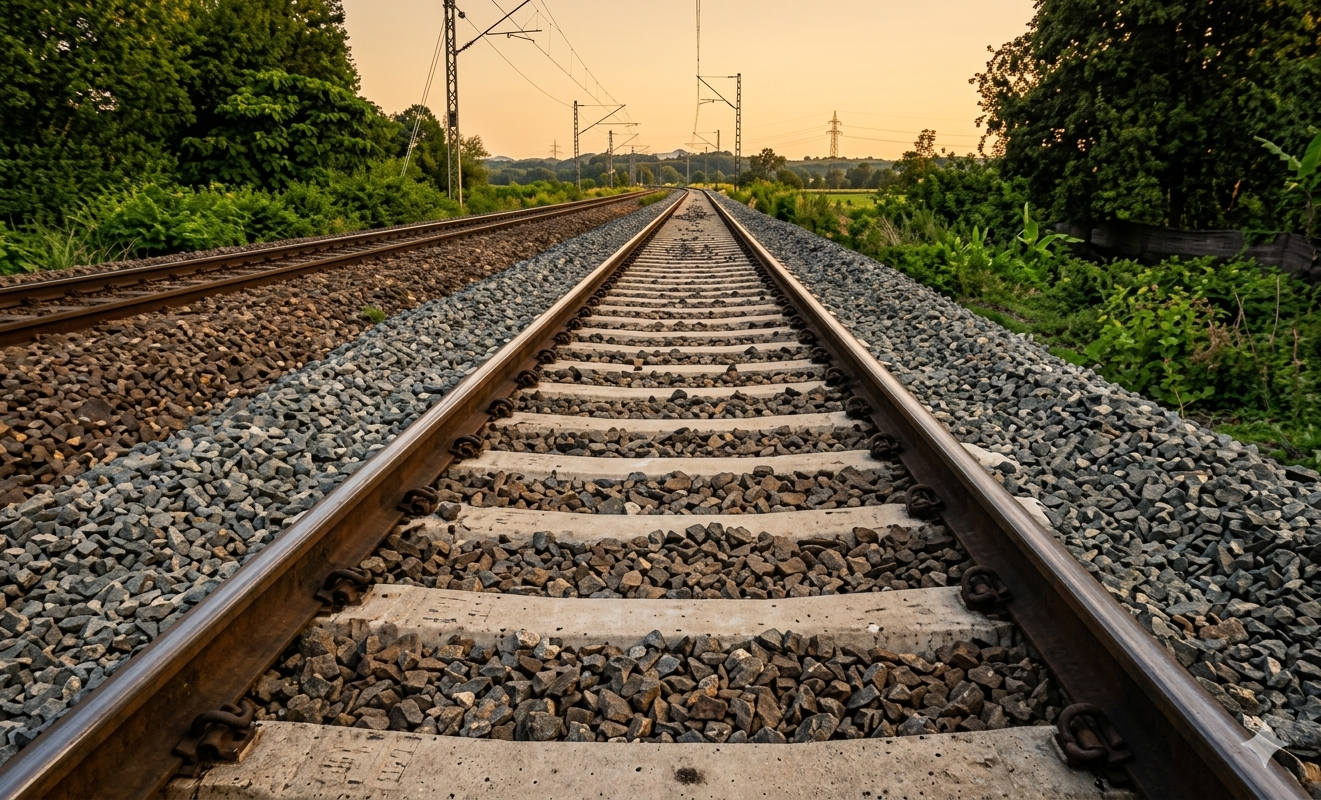
\includegraphics[width=0.85\textwidth]{image4.png}
    \caption{Indian Railways ballasted track in service showing the
             sleeper--ballast system.}
    \label{fig:ballasted-track}
\end{figure}

\begin{figure}[ht]
\centering
\begin{tikzpicture}[>=Stealth,every node/.style={font=\footnotesize}]
    % --- Track structure ---
    % Wheel (circle)
    \draw[thick,fill=gray!40] (0,4.6) circle (0.4);
    \node at (0, 4.6) {\scriptsize $W$};
    \draw[->,very thick,red!80] (0,4.0) -- (0,3.55)
        node[right=2pt,red!80,font=\scriptsize] {wheel load};

    % Rail (small rectangle)
    \draw[thick,fill=gray!60] (-0.8,3.2) rectangle (0.8,3.5);
    \node at (-1.5,3.35) {Rail};

    % Sleeper (long rectangle)
    \draw[thick,fill=brown!30] (-3.0,2.7) rectangle (3.0,3.15);
    \node at (-3.8,2.92) {Sleeper};

    % Ballast layer (trapezoidal-ish)
    \draw[thick,fill=gsvaccent!20] (-3.5,1.6) -- (3.5,1.6) --
                                   (4.0,2.7) -- (-4.0,2.7) -- cycle;
    \node at (-4.8, 2.15) {Ballast};
    % Ballast particles (decorative)
    \foreach \x in {-3,-2.2,-1.5,-0.7,0,0.7,1.5,2.2,3}
        \draw[fill=gray!60] (\x, 2.1) circle (0.18);
    \foreach \x/\y in {-2.6/1.85,-1.8/1.85,-1/1.85,-0.3/1.85,
                       0.4/1.85,1.1/1.85,1.9/1.85,2.6/1.85}
        \draw[fill=gray!50] (\x, \y) circle (0.16);

    % Sub-ballast (lighter)
    \draw[thick,fill=brown!15] (-4.0,1.0) -- (4.0,1.0) --
                               (4.2,1.6) -- (-4.2,1.6) -- cycle;
    \node at (-4.9, 1.3) {Sub-ballast};

    % Subgrade (largest)
    \draw[thick,fill=brown!10] (-4.5,0.0) -- (4.5,0.0) --
                               (4.2,1.0) -- (-4.2,1.0) -- cycle;
    \node at (-5.0, 0.5) {Subgrade};

    % --- Stress trumpet (right side) ---
    \draw[->, very thick, gsvblue]
        (3.6, 3.5) -- (3.6, 1.2) node[right, font=\scriptsize, gsvblue] {depth};
    \draw[gsvblue, very thick] (4.5, 3.3) -- (4.5, 3.0);
    \draw[gsvblue, thick]      (4.3, 2.6) -- (4.7, 2.6);
    \draw[gsvblue]             (4.0, 1.8) -- (5.0, 1.8);
    \draw[gsvblue,thin]        (3.8, 1.0) -- (5.2, 1.0);
    \node[gsvblue,font=\scriptsize\bfseries,anchor=west] at (5.0, 3.15)
        {$\sim$\,500\,kPa};
    \node[gsvblue,font=\scriptsize\bfseries,anchor=west] at (5.0, 2.6)
        {$\sim$\,300\,kPa};
    \node[gsvblue,font=\scriptsize\bfseries,anchor=west] at (5.0, 1.8)
        {$\sim$\,150\,kPa};
    \node[gsvblue,font=\scriptsize\bfseries,anchor=west] at (5.0, 1.0)
        {$\sim$\,80\,kPa};

    % Title
    \node[font=\small\bfseries\color{gsvblue}] at (0, 5.4)
        {Wheel load $\to$ rail $\to$ sleeper $\to$ ballast $\to$ subgrade};
\end{tikzpicture}
\caption{Conceptual diagram of the load-transfer mechanism in
         conventional ballasted track. The vertical wheel load is
         distributed laterally with depth, attenuating from
         $\sim$\,500\,kPa at the top of the ballast to $\sim$\,80\,kPa
         at the subgrade. Ballast degradation under repeated impact
         loading concentrates in the upper $\sim$\,150\,mm of the
         ballast layer where the contact stress is highest.}
\label{fig:load-transfer}
\end{figure}

\section{Problem Statement}
\label{sec:intro-problem}

This thesis addresses two coupled gaps in Indian railway ballast
assessment---gaps that reinforce each other and cannot be closed
independently.

Railroad ballast, typically composed of coarse, angular aggregates, plays a
critical role in providing structural support, stability, and drainage for
railway tracks \citep{Selig1994}. Under repeated train loading, ballast
undergoes degradation through mechanisms such as particle breakage,
abrasion, and fouling, leading to reduced track performance, increased
settlement, and higher maintenance costs. Traditional methods for assessing
ballast degradation, such as sieve analysis and manual inspection, are
time-consuming, labour-intensive, and often subjective, limiting their
scalability and precision. The degradation process is influenced by factors
including impact loading conditions, particle morphology (size, shape, and
surface texture), and environmental variables, yet these interactions are
not fully understood or efficiently quantified.

The primary challenge is the lack of an efficient, objective, and automated
method to assess railroad ballast degradation under realistic loading
conditions. Current drop-weight impact tests simulate train-induced
stresses, but standard protocols do not adequately account for variations
in loading intensity, frequency, or ballast morphological changes over time
\citep{Koohmishi2020}. Moreover, traditional post-test analysis fails to
capture the dynamic evolution of particle characteristics---such as
angularity loss or fragmentation patterns---which are critical to
understanding degradation mechanisms. This gap hinders the ability to
predict ballast performance, optimise maintenance schedules, and design
more durable track systems. There is a need for an innovative approach that
integrates advanced testing conditions with analytical tools to provide a
comprehensive, data-driven assessment of ballast degradation.

\section{Objectives of the Thesis}
\label{sec:intro-objectives}

The thesis pursues five objectives:
\begin{enumerate}[label=(\roman*),leftmargin=*]
    \item To modify the standard drop-weight impact test apparatus (based
          on European standards) to replicate Indian railway ballast
          characteristics and loading conditions.
    \item To evaluate the degradation behaviour of railway ballast under
          repeated impact loading using the modified testing setup.
    \item To investigate the effectiveness of different reinforcement
          conditions in reducing ballast degradation under impact loads.
    \item To quantify morphological changes in degraded ballast particles
          using 3D image processing techniques (shape, angularity, and size
          variations).
    \item To establish relationships between impact-induced degradation and
          morphological characteristics for improved assessment of ballast
          performance.
\end{enumerate}

\section{Scope}
\label{sec:intro-scope}

The scope of this thesis focuses on the experimental and analytical
investigation of railway ballast degradation under controlled impact
loading conditions, with particular emphasis on adapting existing testing
methodologies to Indian railway requirements. The study involves modifying
and calibrating a drop-weight impact test apparatus, originally based on
European standards, to simulate realistic loading conditions representative
of Indian Railways, including higher axle loads and varying traffic
characteristics. Laboratory experiments are conducted to evaluate ballast
degradation behaviour under repeated impact loading, examining parameters
such as particle breakage, gradation changes, and degradation indices. In
addition, the research assesses the effectiveness of selected reinforcement
or stabilisation techniques in reducing ballast deterioration. A key
component of the study is the application of advanced three-dimensional
image-processing methods to quantify changes in ballast particle
morphology, including shape, angularity, and surface characteristics before
and after degradation. The thesis further aims to establish correlations
between mechanical degradation and morphological evolution of ballast
particles, contributing to improved understanding of ballast performance.
However, the study is limited to laboratory-scale investigations, specific
ballast types used in Indian Railways, and impact loading conditions,
without extensive consideration of long-term field performance or
environmental effects.

\section{Thesis structure}
\label{sec:intro-structure}

The remainder of the thesis is organised as follows.
\cref{chap:literature} reviews the literature on ballast degradation
mechanisms, laboratory characterisation under impact loading,
substructure reinforcement, and three-dimensional morphological
characterisation, and identifies the two gaps the present work is
designed to fill. \cref{chap:methodology} documents the materials,
apparatus, calibration, test protocol, and morphological-analysis
pipeline. \cref{chap:impact-results} reports the bulk-specimen response
(settlement, peak hammer force, Indian Railway Fouling Index \FIIN) for
the nine-configuration programme. \cref{chap:morph-results} reports the
paired per-particle morphological response across twenty-two descriptors
for the 45 tracer particles, with a particular focus on the
\gls{ModeA}~/~\gls{ModeB} dichotomy. \cref{chap:conclusions} states the
principal conclusions, the novel contributions, the limitations, and the
recommendations for future work.

\begin{figure}[ht]
    \centering
    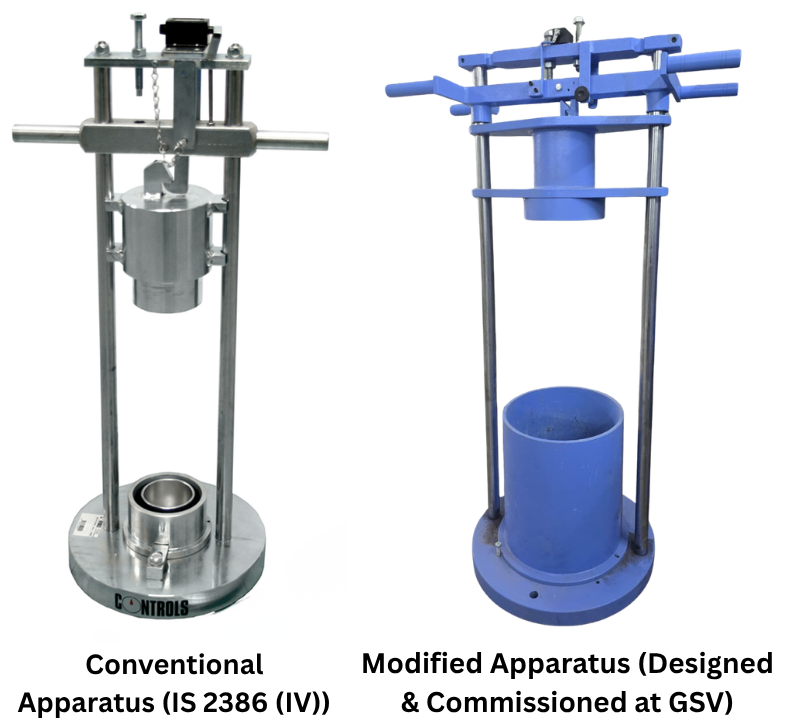
\includegraphics[width=0.95\textwidth]{image5.png}
    \caption{Comparison of the modified impact-testing apparatus designed
             and commissioned at \gls{GSV} against the conventional
             aggregate impact value apparatus.}
    \label{fig:apparatus-comparison}
\end{figure}

% =============================================================================
%  CHAPTER 2 - LITERATURE REVIEW
% =============================================================================
\chapter{Literature Review}
\label{chap:literature}

The literature on ballast degradation is both deep and unusually fragmented.
It is deep because serious laboratory work on granular skeletons under cyclic
and impact loading has been continuous since the 1960s, and it has been
reinforced in the last two decades by discrete-element modelling, by field
monitoring of mainline track, and---most recently---by three-dimensional
imaging of individual grains. It is fragmented because these different
strands have grown largely independently of one another: the cyclic-triaxial
community and the impact community have different journals and different
index vocabularies; the image-analysis community has only recently made
sustained contact with the degradation-mechanics community; and the
practitioners who set national ballast specifications have, in turn, moved at
their own pace. This review is organised thematically rather than
paper-by-paper in order to make sense of these strands together.

Six themes are traced in turn. Section~\ref{sec:lit-layer} places the ballast
layer in the track system and reviews its functional requirements.
Section~\ref{sec:lit-degradation} discusses the mechanisms of ballast
degradation that the thesis is ultimately concerned with.
Section~\ref{sec:lit-lab} examines the laboratory characterisation of
degradation under cyclic and impact loading, with particular attention to the
apparatus and the size-effect problem that motivates Chapter~3.
Section~\ref{sec:lit-reinforcement} reviews the use of resilient substructure
inclusions---pads, mats, and compliant bases---to intercept and dissipate the
impulsive energy that drives grain-scale damage.
Section~\ref{sec:lit-morphology} surveys the emergence of three-dimensional
morphological characterisation, which supplies the measurement framework
used in Chapter~3 and applied in Chapter~5.
Section~\ref{sec:lit-synthesis} draws the preceding five sections together
and identifies the two gaps---the apparatus gap and the characterisation
gap---that this thesis addresses.

\section{The ballast layer in the railway track system}
\label{sec:lit-layer}

\subsection{Functional requirements}
\label{sec:lit-functional}

The conventional ballasted track is a layered granular--structural system
whose task is to convert the concentrated contact forces at the wheel--rail
interface into diffuse, tolerable stresses at the subgrade surface. The
ballast layer---a \SIrange{250}{350}{\milli\metre} deep mat of crushed,
angular stone placed beneath and around the sleepers---is the principal
load-distributing element of this system. Selig and Waters (1994) enumerated
its six primary functions: (i) distribution of vertical wheel loads from the
sleepers to the subgrade over an area substantially larger than the sleeper
footprint; (ii) restraint against lateral and longitudinal sleeper movement
through inter-particle friction and interlock; (iii) absorption of some
fraction of the dynamic energy imparted by passing trains; (iv) provision of
rapid drainage of water away from the track formation; (v) accommodation of
tamping and lining operations without structural damage; and (vi)
maintenance of a resilient bearing surface that allows the rail to deflect
elastically under load without plastic accumulation at the sleeper--ballast
contact.

These six functions impose mutually constraining requirements on the
material. High lateral restraint demands angular, machine-crushed grains
with strong inter-particle interlock; high drainage demands a uniformly
graded, coarse assembly with open voids; load distribution demands adequate
depth and density; and long service life demands particles hard enough to
resist both impact-driven fracture and cumulative abrasion. These
requirements are reflected in national ballast specifications with
remarkable consistency: AREMA (2020) in the United States, UIC~719R in
continental Europe, and the RDSO specification (RDSO, 2023) in India all
prescribe crushed, angular stone of comparable hardness and in a comparable
\SIrange{20}{65}{\milli\metre} size band, albeit with local variations in
the permissible fines fraction and in the tolerated parent-rock types.

A small but growing body of Indian-context research has begun to address the
specific behaviour of RDSO-gradation ballast. Gundavaram and Hussaini (2023)
--- the present supervisor --- demonstrated in cyclic triaxial tests on
elastomeric-polyurethane-reinforced ballast that the inclusion of a
polymeric element between the ballast and the subgrade substantially reduces
cumulative plastic deformation and attenuates the growth of the fines
fraction. That result, on cyclic loading, motivates in part the use of the
polyurethane under-ballast mat (PUBM) condition in the present impact-loading
study.

\section{Ballast Degradation}
\label{sec:lit-degradation}

\subsection{Fouling and its engineering consequences}
\label{sec:lit-fouling}

The engineering consequence of the three grain-scale mechanisms is the
progressive generation of fines---particles finer than
\SI{0.075}{\milli\metre} in the Selig and Waters (1994) usage, or finer than
the RDSO \SI{0.075}{\milli\metre} sieve in the Indian adaptation. These
fines infill the voids of the ballast skeleton and give rise to the condition
known as \textit{fouling}. A fouled ballast has reduced drainage capacity,
reduced shear strength, a softer and more plastic response to cyclic load,
and a higher rate of settlement under repeated traffic (Huang et~al., 2009;
Tutumluer, 2013). The practical maintenance responses---ballast cleaning,
partial renewal, and in extreme cases full deep-screening---are costly and
disruptive, and the engineering motivation for slowing the rate of fines
generation is direct and economic.

Field fouling has an exogenous contribution---coal and mineral-ore spillage
from freight wagons, wind-blown dust, and subgrade pumping---that is not
reproducible in a sealed laboratory mould. The laboratory characterisation
of degradation therefore measures the endogenous contribution only. Within
the laboratory, the self-generated fouling contribution is quantified by a
family of bulk indices whose development and limitations are reviewed next.

\subsection{Fouling Index}
\label{sec:lit-fouling-index}

The Fouling Index $\mathit{FI}=P_{4}+P_{20}$, introduced by Selig and Waters
(1994), and its metric counterpart $\FIIN=\PoneM+\PtwoM$ adapted for Indian
conditions by Anbazhagan, Lijun, Bharatha, and Pratibha (2012), are weighted
sums of the percentages finer than key sieves and are intended to capture
the fines-generation aspect of degradation specifically rather than the
total PSD shift. The fouling index is dimensionless, is reported in weight
percent, and is the bulk metric most directly tied to the engineering
consequences that motivate ballast replacement in the field---loss of
drainage, loss of shear strength, and the progressive infilling of voids
that drives settlement-bowl formation at impact-prone locations. Because it
isolates the fines fraction and the sub-acceptable fraction, \FIIN{} is also
the most widely reported degradation metric in the Indian-ballast literature
and is referenced (in its imperial form) in international ballast-fouling
specifications.

\begin{equation}
    \FIIN = \PoneM + \PtwoM
    \label{eq:FIIN-def}
\end{equation}

\FIIN{} is a scalar summary of the post-test particle-size distribution and
therefore carries a structural blind spot common to any sieve-derived index.
Two test specimens can produce identical \FIIN{} values while differing in
the grain-scale distribution of damage: one specimen may have experienced a
small amount of abrasion distributed across all its grains, another may
have experienced catastrophic fracture of a few geometrically weak grains
with the remainder largely untouched. If the two damage patterns happen to
push comparable fractions across the \SI{0.075}{\milli\metre} and
\SI{20}{\milli\metre} sieves, the index reports the same value. The two
specimens have the same post-test PSD in those two bands, the same \FIIN{},
and completely different underlying physical states. The engineering
implications---for settlement, for the spatial distribution of fines, for
void fabric, for drainage---are not the same.

\subsection{Factors affecting ballast breakage and its propagation}
\label{sec:lit-breakage}

The rate and mode of ballast breakage are not properties of the rock alone
but emerge from the interaction of intrinsic material variables with
extrinsic loading and boundary variables. The intrinsic variables include
the parent-rock mineralogy and grain texture, the unconfined compressive and
tensile strengths, the density of pre-existing micro-cracks, and---at the
assembly scale---the particle size distribution and the particle shape
(angularity, sphericity and flatness/elongation). The extrinsic variables
include the magnitude and frequency of the applied load, the stress path
(monotonic versus cyclic, confined triaxial versus impact), the moisture
state, the degree of confinement provided by adjacent layers, and the
stiffness of the substructure on which the ballast rests. Indraratna et~al.\
(2011) and Sun, Indraratna, and Nimbalkar (2014) summarise these dependencies
and show that, holding intrinsic properties constant, the breakage index
rises sharply with peak stress and with the number of load cycles, but is
moderated by confining pressure (which suppresses tensile failure at point
contacts) and by the introduction of a resilient layer beneath the ballast
(which lengthens the contact pulse and lowers its peak).

At the grain scale the propagation of breakage is controlled by the geometry
of the contact and the distribution of pre-existing micro-flaws within the
parent rock. Hertzian contact theory predicts a tensile-stress lobe just
below a point or near-point contact whose magnitude scales with the contact
force to the one-third power; once this tensile stress exceeds the local
tensile strength, a crack initiates and propagates along the path of least
resistance through the grain (Lim \& McDowell, 2005). Angular grains contact
each other over small areas and therefore generate higher contact stresses
for a given force, which is why fresher, more angular ballast fractures
preferentially in the early loading history before transitioning to an
abrasion-dominated regime. Conversely, more rounded grains distribute the
same contact force over a larger area, reduce the peak tensile stress, and
shift the dominant degradation mode toward asperity wear. The stiffness of
the substructure beneath the ballast plays an analogous role at the layer
scale: a stiffer base concentrates contact forces at fewer particle--particle
and particle--base contacts, while a resilient inclusion (rubber pad,
under-sleeper pad, or under-ballast mat) lengthens the contact-force pulse
and reduces its peak, biasing the degradation toward abrasion and away from
fracture (Sol-S\'anchez, Moreno-Navarro, \& Rubio-G\'amez, 2015;
Navaratnarajah \& Indraratna, 2017).

Propagation through the assembly is governed by force-chain mechanics rather
than by the average stress. Discrete-element simulations and photoelastic
studies of granular media (Cundall \& Strack, 1979; Tordesillas, 2007) show
that load is transmitted through a sparse network of strong contacts that
carry well above the mean stress, while the remaining particles bear
comparatively little load. Particles that lie on a strong force chain
experience contact stresses that can exceed the bulk-applied stress by an
order of magnitude and are therefore the first to fracture. When such a
particle splits, the chain rearranges; load is shed onto neighbouring
particles, which may themselves fracture in the next loading cycle,
producing a cascade until a stable contact network re-forms. This
force-chain rearrangement is the mechanism by which breakage is spatially
clustered rather than uniformly distributed, and it explains the field
observation that fines are often concentrated in localised pockets within an
otherwise comparatively intact ballast layer.

A second statistical layer concerns the variability of breakage outcomes
between nominally identical particles. Single-particle crushing tests on
ballast and rockfill consistently report a wide scatter in the failure load
even within a narrow size band, and the distribution is well described by
Weibull statistics with a modulus typically in the range \numrange{3}{6} for
basaltic and granitic ballast (McDowell, 2002; Lim, McDowell, \& Collop,
2004). The Weibull modulus encodes the heterogeneity of internal flaws:
lower moduli indicate that a small population of weak particles will
fracture early in the loading history, while the bulk of the assembly
continues to degrade by abrasion. This is consistent with the bimodal damage
pattern observed in laboratory specimens, where a few catastrophically split
particles coexist with a majority showing only corner rounding, and it sets
a lower bound on how representative any single test outcome can be of the
assembly response.

\section{Laboratory characterisation of ballast under impact loading}
\label{sec:lit-lab}

\subsection{Impact-loading studies and the size-of-mould problem}
\label{sec:lit-impact-mould}

Impact loading---as distinct from cyclic-triaxial loading---has received
less sustained attention, despite being the loading mode that dominates at
impact-prone locations in service. The seminal study of Nimbalkar,
Indraratna, Dash, and Christie (2012) used a \SI{300}{\milli\metre} diameter
drop-weight rig with a \SI{50}{\kilogram} falling hammer and a
\SI{500}{\milli\metre} drop height to establish that shock mats placed
beneath the ballast reduce post-test bulk degradation substantially, and
that the benefit of the shock mat is greatest when the underlying support is
rigid. The same authors subsequently demonstrated that recycled rubber mats
achieve comparable performance at much lower cost. This line of
inquiry---large-diameter mould, drop-weight hammer, ballast-scale
particles---is the line that the present apparatus continues.

A series of papers by Koohmishi and co-workers has extended the drop-weight
methodology in several directions. Koohmishi and Palassi (2020) investigated
the morphological response of basalt, granite, limestone and a
mixed-lithology ballast under drop-weight impact and showed that the parent
rock type governs the partition of damage between abrasion and splitting.
Koohmishi and Azarhoosh (2021, 2022) studied the effect of crumb-rubber
incorporation on both fresh and recycled ballast, finding that
\SIrange{5}{10}{\percent} rubber by volume reduces post-test bulk breakage
measurably but that the benefit saturates---and eventually reverses---beyond
about \SI{15}{\percent}. Koohmishi and Guo (2023) combined drop-weight
impact data with random-forest and support-vector-regression models and
demonstrated that parent rock type and nominal impact stress together
explain the majority of variance in post-test bulk degradation, with rubber
content contributing an additional smaller effect. Zhang, Chang, and Feng
(2023) and the very recent Chen, Zhang, Yang, and Wu (2026) have continued
this line on ballast--rubber mixtures, with the 2026 study being the first
to explicitly couple impact-loading breakage to the gradation-evolution
trajectory during a multi-blow test rather than only at the endpoint.

Across all of these studies the same apparatus-related problem appears: the
conventional IS/BS aggregate impact value test (BIS, 1963; BSI, 2010) has a
\SI{102}{\milli\metre} diameter mould that is far too small for
RDSO-gradation ballast. Marsal (1967) established that the boundary
conditions of a granular test dominate the measured response until the
container diameter is at least six times the maximum particle size, and
Bishop (1969) independently reached a similar conclusion from work on
rock-skeleton saturation response. In a \SI{102}{\milli\metre} mould with
\SIrange{40}{65}{\milli\metre} particles the ratio is
\numrange{1.6}{2.5}---one is no longer testing the ballast, one is testing
the mould wall. The universal response in the published impact literature
has been to develop purpose-built large-diameter rigs of
\SIrange{250}{500}{\milli\metre} diameter (e.g.\ Nimbalkar et~al., 2012;
Koohmishi \& Palassi, 2020; Ferreira \& Indraratna, 2023)---but none of
these has been designed or calibrated specifically for the RDSO gradation
and the Indian stress range, and none is standardised for Indian Railways
quality assurance. The present thesis fills that specific apparatus gap.

\begin{figure}[ht]
    \centering
    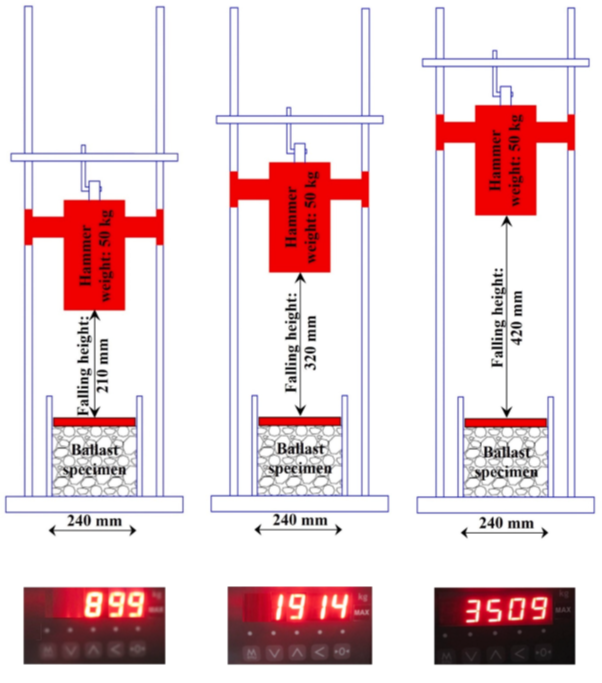
\includegraphics[width=0.80\textwidth]{image6.png}
    \caption{Established falling height through the impact loading test for
             implementing the characterised stress levels on ballast
             (Koohmishi \& Guo, 2023).}
    \label{fig:koohmishi-falling-height}
\end{figure}

\begin{table}[ht]
\centering
\caption{Representative drop-weight impact studies on railway ballast:
         apparatus and method comparison.}
\label{tab:lit-impact-studies}
\small
\begin{adjustbox}{max width=\textwidth}
\begin{tabular}{@{}lcccp{3.0cm}p{2.6cm}p{2.4cm}@{}}
    \toprule
    \textbf{Study} & \textbf{Mould $D$} & \textbf{Hammer} & \textbf{Drop $h$}
    & \textbf{Variables} & \textbf{Metrics} & \textbf{Ballast}\\
    \midrule
    Nimbalkar et~al.\ (2012)  & \SI{300}{\mm} & \SI{50}{\kg}
        & \SI{500}{\mm} & Shock mats, various
        & \FIIN & AU freight ballast\\
    Koohmishi \& Palassi (2020) & \SI{250}{\mm} & \SI{40}{\kg}
        & Variable & Crumb rubber, rock types
        & \FIIN & Mixed (basalt, granite, limestone)\\
    Koohmishi \& Azarhoosh (2021) & \SI{250}{\mm} & \SI{40}{\kg}
        & Variable & Crumb rubber + gradation
        & \FIIN & Recycled ballast\\
    Koohmishi \& Azarhoosh (2022) & \SI{250}{\mm} & \SI{40}{\kg}
        & Variable & Crumb rubber + recycling
        & \FIIN & Recycled ballast\\
    Zhang et~al.\ (2023) & \(\sim\!\SI{300}{\mm}\) & \SI{45}{\kg}
        & \SI{450}{\mm} & Crumb rubber, energy
        & \FIIN, image analysis & Basalt\\
    Ferreira \& Indraratna (2023) & \SI{300}{\mm} & \SI{50}{\kg}
        & \SI{450}{\mm} & Image-based morphology
        & 2D morphology, FI & Australian ballast\\
    \textbf{Present study} & \SI{300}{\mm} & \SI{50}{\kg}
        & Variable & UR / RUBM / PUBM $\times$ FB / RB
        & \FIIN{} + 3D morphology (paired) & Indian Ballast\\
    \bottomrule
\end{tabular}
\end{adjustbox}
\end{table}

Table~\ref{tab:lit-impact-studies} makes two observations explicit. First,
the dominant apparatus tradition has converged on a
\SIrange{250}{300}{\milli\metre} mould, a \SIrange{40}{50}{\kilogram}
hammer, and drop heights in the \SIrange{300}{500}{\milli\metre} range---all
broadly consistent with the present apparatus described in
Chapter~\ref{chap:methodology}. Second, the metrics reported are
overwhelmingly sieve-based bulk metrics, with image-based morphology
appearing only in the two most recent studies and in neither case as a
paired before--after protocol on individually marked tracer particles. The
present thesis is, to the authors' knowledge, the first to combine a
large-diameter drop-weight apparatus calibrated for RDSO gradation with a
fully paired per-particle three-dimensional morphological characterisation
across a factorial grid of pad type, base condition and impact energy.

\section{Ballast Reinforcement Methods}
\label{sec:lit-reinforcement}

Three categories of inclusion are commonly used to reinforce or protect the
ballast layer: under-sleeper pads (USPs), which sit between the sleeper and
the ballast; under-ballast mats (UBMs), which sit beneath the ballast and
above the sub-ballast or subgrade; and geogrids, planar polymeric grids
embedded within or beneath the ballast that confine particles through
aperture interlock. The first two add compliance at a stiffness-mismatched
interface to attenuate impact energy, whereas geogrids reinforce the ballast
layer mechanically by restraining lateral spread of the granular skeleton.

Their mechanical regimes differ in kind. USPs are stiff elastomeric layers
bonded to the underside of the sleeper that reduce sleeper--ballast contact
stress, with static stiffness typically in the
\SIrange{0.10}{0.30}{\newton\per\milli\metre\cubed} band (Jayasuriya et~al.,
2019). UBMs are placed beneath the ballast to attenuate impact energy
transmitted to the subgrade; rubber variants cover roughly
\SIrange{0.02}{0.10}{\newton\per\milli\metre\cubed} (Navaratnarajah \&
Indraratna, 2017; Ngo et~al., 2019), and the polyurethane UBM (PUBM) used in
the present study spans a wider product range. Geogrids, by contrast, are
planar polymeric grids embedded within or beneath the ballast that confine
particles through aperture interlock; they slow lateral spread of the
granular skeleton and the rate of fines generation under repeated loading.
Choosing among these three is therefore a question of matching mechanism to
the dominant local issue---stress reduction at the sleeper interface, energy
attenuation above the subgrade, or particle confinement within the ballast
itself---rather than of selecting the most compliant element available.

\section{Three-dimensional morphological characterisation of ballast}
\label{sec:lit-morphology}

\subsection{From sieve-based to shape-based descriptors}
\label{sec:lit-sieve-to-shape}

The classical sieve-based characterisation of a ballast sample---its PSD and
any index derived from it---does not resolve particle shape. Two assemblies
with identical PSDs can differ substantially in the angularity, elongation,
and surface texture of their grains, and the difference in shape is known to
affect both initial strength and degradation kinetics. The classical
shape-analysis literature begins with Wadell (1932), who introduced the
concept of sphericity $\Psi$ as the ratio of the surface area of a
volume-equivalent sphere to the actual surface area of the particle:
\begin{equation}
    \Psi = \frac{\pi^{1/3}\,(6V)^{2/3}}{A},
    \label{eq:sphericity}
\end{equation}
and with Krumbein (1941), who extended the framework to sedimentary particle
populations.

\begin{figure}[ht]
    \centering
    \begin{subfigure}{0.48\textwidth}
        \centering
        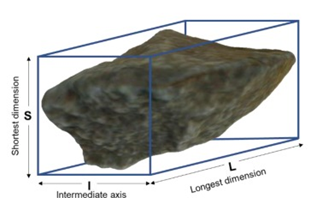
\includegraphics[width=\linewidth]{image7.png}
        \caption{Ballast scanning methodology.}
    \end{subfigure}\hfill
    \begin{subfigure}{0.48\textwidth}
        \centering
        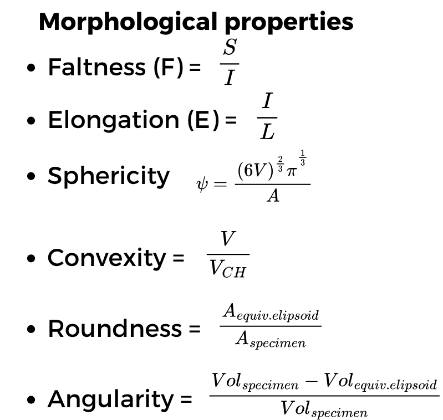
\includegraphics[width=\linewidth]{image8.png}
        \caption{Principal $S$, $I$, $L$ dimensions.}
    \end{subfigure}
    \caption{Morphological parameters and the $S$, $I$, $L$ bounding-box
             dimensions of a ballast particle.}
    \label{fig:morph-params}
\end{figure}

\subsection{The rise of structured-light scanning}
\label{sec:lit-sl-scanning}

The second-generation shape-characterisation moved from manual calliper
measurement to digital imaging. Sun, Indraratna, and Nimbalkar (2014a)
applied three-dimensional laser scanning to the size and shape of
as-supplied quarry ballast and produced one of the first systematic datasets
of paired particle volumes and surface areas. Qian, Boler, Moaveni,
Tutumluer, Hashash, and Ghaboussi (2014) coupled image analysis to Los
Angeles abrasion testing and showed that abrasion in the LAA mill follows a
characteristic angularity-decay trajectory that can be tracked
particle-by-particle. Guo, Markine, Song, and Jing (2018) refined the
angularity-index concept and, with the same LAA methodology, demonstrated
that the size- and shape-dependence of degradation can be quantified at the
single-particle level.

The tool-chain that supports this line of work has matured rapidly.
Angelidakis, Nadimi, and Utili (2021) released an open-source shape-analysis
code (SHAPE) that computes a standardised set of form and roundness
descriptors from triangulated surface meshes. The open-source Python
mesh-processing library \texttt{trimesh} (Dawson-Haggerty, 2019) has become
the de-facto workhorse for reading and interrogating STL files, and the
scientific-computing stack NumPy and SciPy (Harris et~al., 2020; Virtanen
et~al., 2020) supports the downstream statistical analysis. Kwunjai, Somsri,
Jitsangiam, Binaree, Qian, and Jing (2023) combined a structured-light
scanning workflow with supervised machine learning to classify deteriorated
ballast and demonstrated that grain-scale shape descriptors carry the
information required to distinguish fresh from service-aged ballast.
Kwunjai, Jitsangiam, and Somsri (2024) simplified the analysis pipeline
while retaining the essential descriptor set.

\subsection{Paired before--after protocols}
\label{sec:lit-paired}

The crucial methodological step---and the one that the present thesis is
built on---is the paired before--after protocol. If the same physical grains
are characterised before and after a loading event, then each grain serves
as its own pre-test control and the particle-to-particle variability that is
the dominant source of scatter in unpaired datasets is eliminated. The
paired protocol has been used occasionally in the literature, most notably
by Ferreira and Indraratna (2023) for two-dimensional image analysis of
ballast under impact loading and by Bian, Cai, Luo, Zhao, and Chen (2023)
for in-situ image-aided analysis of ballast particle movement along a
high-speed railway. It has not, however, been applied in combination with a
large-diameter drop-weight apparatus across a factorial grid of pad type,
base condition, and impact energy, which is the methodological novelty of
the present study.

\section{Synthesis and identification of gaps}
\label{sec:lit-synthesis}

Three synthesising observations emerge from the preceding five sections, and
together they identify the two gaps that this thesis is designed to fill.

\subsection{Synthesising observations}
\label{sec:lit-synth-obs}

\begin{enumerate}[label=(\arabic*),leftmargin=*]
    \item The dominant laboratory apparatus tradition for impact loading of
          ballast has converged on \SIrange{250}{300}{\milli\metre} mould,
          \SIrange{40}{50}{\kilogram} hammer, \SIrange{300}{500}{\milli\metre}
          drop-height rigs that satisfy the $D/\dmax \ge 6$ boundary
          criterion. However, no apparatus in the public record has been
          designed or calibrated specifically for the RDSO
          \SIrange{20}{65}{\milli\metre} gradation and the
          \SIrange{275}{525}{\kilo\pascal} stress range representative of
          Indian Railways---the very specification and stress band that
          governs acceptance of ballast for the Indian network.
    \item The dominant characterisation tradition---the Fouling Index, in
          its imperial and metric forms---is bulk in character and cannot,
          by construction, distinguish diffuse abrasion from catastrophic
          single-particle fracture. Two specimens with identical \FIIN{}
          values can have very different grain-scale damage patterns, with
          different implications for settlement-bowl formation and
          maintenance scheduling.
    \item The emerging three-dimensional morphological tradition has
          demonstrated that per-particle before--after characterisation is
          technically feasible and methodologically sound, but has not yet
          been combined with a large-diameter drop-weight apparatus across a
          factorial grid of pad type, base condition, and impact energy---the
          very grid that is most relevant to the practical design of
          resilient inclusions at impact-prone locations on a national rail
          network.
\end{enumerate}

% =============================================================================
%  CHAPTER 3 - MATERIALS AND METHODOLOGY
% =============================================================================
\chapter[Methodology]{Materials and Methodology}
\label{chap:methodology}

\chapterquote{If you cannot weigh, measure, or photograph it, you cannot
yet engineer it.}{after Lord Kelvin, 1883}

\begin{chapterpreview}
This chapter documents in reproducible detail the apparatus, the
materials, and the protocol used in the experimental programme.
\cref{sec:meth-materials} characterises the basalt ballast and verifies
its conformity to the \gls{RDSO} gradation envelope.
\cref{sec:meth-PUBM,sec:meth-RUBM} specify the two under-ballast mat
materials. \cref{sec:meth-apparatus} describes the modified large-scale
drop-weight impact apparatus (Figure~\ref{fig:meth-flowchart}).
\cref{sec:meth-calibration} calibrates the apparatus against the
Indian Railways field-stress envelope. \cref{sec:meth-protocol} fixes
the assembly and blow protocol; \cref{sec:meth-matrix} sets out the
nine-cell factorial test matrix (Figure~\ref{fig:meth-matrix}). The
chapter ends with the twenty-two-descriptor per-particle pipeline
(\cref{sec:meth-morphology,sec:meth-descriptors}).
\end{chapterpreview}

\dropcap{T}{his} chapter documents the materials, the apparatus, the test protocol, and
the per-particle morphological-analysis pipeline used in the experimental
programme. The chapter is the longest in the thesis because the programme
combines two methodological strands---bulk-index testing through a modified
drop-weight impact apparatus, and paired three-dimensional morphological
characterisation of individually marked tracer particles---and
reproducibility of either strand requires a fully specified procedure. The
chapter is organised into eight sections following the natural workflow of
the programme: materials (Section~\ref{sec:meth-materials}), pad and base
conditions (Section~\ref{sec:meth-reinforcement}), tracer-particle
preparation (Section~\ref{sec:meth-scanning}), the modified drop-weight
impact apparatus (Section~\ref{sec:meth-apparatus}), stress-and-energy
calibration to Indian Railways field loading
(Section~\ref{sec:meth-calibration}), the blow-by-blow test protocol and
bulk-index computation (Section~\ref{sec:meth-protocol}), and the image-based
three-dimensional morphological-analysis pipeline
(Section~\ref{sec:meth-morphology}).

\begin{figure}[ht]
\centering
\begin{tikzpicture}[node distance=0.5cm and 0.6cm,>=Stealth]
    % -------- Bulk stream (left column) --------
    \node[flowstart]                                            (start)    {Source basalt ballast (RDSO gradation)};
    \node[flowstep, below=of start]                             (sieve-in) {Dry-sieve analysis\\(pre-test PSD)};
    \node[flowstep, below=of sieve-in]                          (prep)     {Specimen assembly\\(mould + base + pad + 20\,kg fill)};
    \node[flowstep, below=of prep]                              (impact)   {Drop-weight impact test\\(20 blows; 300 or 450\,mm drop)};
    \node[flowstep, below=of impact]                            (sett)     {Settlement \& peak force\\(every 5 blows)};
    \node[flowstep, below=of sett]                              (sieve-out){Post-test sieve analysis\\(RDSO series)};
    \node[flowstep, below=of sieve-out]                         (fiin)     {Compute $\FIIN = \PoneM + \PtwoM$};

    % -------- Per-particle stream (right column) --------
    \node[flowstep, right=2.6cm of prep]                        (select)   {Select 5 tracer particles\\per configuration ($n=45$)};
    \node[flowstep, below=of select]                            (scanbef)  {Pre-test 3D scan\\(EinScan SL, $\sim$0.1\,mm)};
    \node[flowstep, below=of scanbef]                           (qcbef)    {QC: watertight,\\single body, vol.\ in band};
    \node[flowstep, below=of qcbef]                             (extract)  {Recover tracers post-test,\\re-scan, QC};
    \node[flowstep, below=of extract]                           (desc)     {Compute 22 descriptors\\and paired $\Delta X$, $\%\Delta X$};

    % Synthesis box
    \node[flowend, below=2.2cm of $(fiin)!0.5!(desc)$]          (synth)    {Synthesis (\FIIN{} + paired morphology)};

    % -------- Arrows --------
    \draw[flowarrow] (start)    -- (sieve-in);
    \draw[flowarrow] (sieve-in) -- (prep);
    \draw[flowarrow] (prep)     -- (impact);
    \draw[flowarrow] (impact)   -- (sett);
    \draw[flowarrow] (sett)     -- (sieve-out);
    \draw[flowarrow] (sieve-out)-- (fiin);
    \draw[flowarrow] (fiin)     |- (synth);

    \draw[flowarrow] (select)   -- (scanbef);
    \draw[flowarrow] (scanbef)  -- (qcbef);
    \draw[flowarrow, dashed]    (qcbef.south)
        .. controls +(0,-0.4) and +(2.5,0) ..
        (prep.east) node[midway,above,font=\scriptsize\itshape] {tracers go in};
    \draw[flowarrow, dashed]    (impact.east)
        .. controls +(2.5,0) and +(0,0.4) ..
        (extract.north) node[midway,below,font=\scriptsize\itshape] {tracers come out};
    \draw[flowarrow] (extract)  -- (desc);
    \draw[flowarrow] (desc)     |- (synth);

    % Stream labels
    \node[font=\small\bfseries\color{gsvblue}, above=0.2cm of start]
        {Bulk stream};
    \node[font=\small\bfseries\color{gsvblue}, above=0.2cm of select]
        {Per-particle stream};
\end{tikzpicture}
\caption{Experimental methodology: a two-stream pipeline. The bulk stream
         (left) follows the specimen through assembly, impact testing,
         and post-test sieve analysis, ending in the Indian Railway
         Fouling Index \FIIN. The per-particle stream (right) follows 45
         individually-tracked tracer particles through 3D scanning,
         quality control, impact loading, re-scan, and 22-descriptor
         comparison. The two streams converge in the synthesis stage.}
\label{fig:meth-flowchart}
\end{figure}

\section{Basalt ballast}
\label{sec:meth-materials}

\subsection{Source and parent rock}
\label{sec:meth-source}

All ballast used in the experimental programme was sourced from a single
quarry supplying \gls{RDSO}-specification railway ballast in the Vadodara
region of Gujarat, India. A single source was used to eliminate parent-rock
variability as a confounding factor between tests: any cross-test difference
in degradation can then be attributed to the reinforcement configuration
rather than to unrecorded mineralogical variation. The parent rock is
basalt---a fine-grained, dense, aphanitic igneous rock with a dry particle
density \SI{2.76}{\gram\per\centi\metre\cubed} and low water absorption
(\(<\SI{1}{\percent}\)). These figures are consistent with the \gls{RDSO}
specification \citep{RDSO2023} requirement of not less than
\SI{2.60}{\gram\per\centi\metre\cubed} dry density and with the parent-rock
properties reported for comparable basalt in the impact literature
\citep{Koohmishi2020, Zhang2023}.

Approximately \SI{25000}{\kilogram} of ballast was procured for the
programme---much more than required for the nine main tests (approximately
\SI{20}{\kilogram} each), for the preliminary calibration trials run during
apparatus commissioning, and for a replacement reserve. All nine tests
therefore drew from the same stockpile and the same parent rock. The
stockpile was kept covered and elevated from direct ground contact between
tests to prevent contamination of the void-fouling baseline.

\subsection{Particle size distribution and the RDSO envelope}
\label{sec:meth-psd}

The as-supplied ballast was characterised by dry-sieve analysis using the
following sieve series: 63, 50, 40, 31.5, 25, 20, 16, 12.5, 10, 4.75, 2.36,
0.6, 0.15 and \SI{0.075}{\milli\metre}. Sieving was performed on sample
masses of approximately \SI{10}{\kilogram} in accordance with the spirit of
the \gls{RDSO} procedure \citep{RDSO2023}. The resulting gradation, plotted
in \cref{fig:meth-psd} against the \gls{RDSO} upper and lower envelope
curves, shows that the ballast conforms to the specification with a small
reserve against both limits---the target gradation sits close to the mid-band
of the envelope throughout the \SIrange{20}{63}{\milli\metre} range. The
percentage retained on the \SI{65}{\milli\metre} sieve was below the
\SI{5}{\percent} maximum permitted by the specification; the percentage
passing the \SI{20}{\milli\metre} sieve was below \SI{2}{\percent}, well
within the \SI{2}{\percent} maximum fines limit. The gradation is therefore
centred within the acceptable window and is representative of
production-quality \gls{RDSO} ballast.

\begin{figure}[ht]
    \centering
    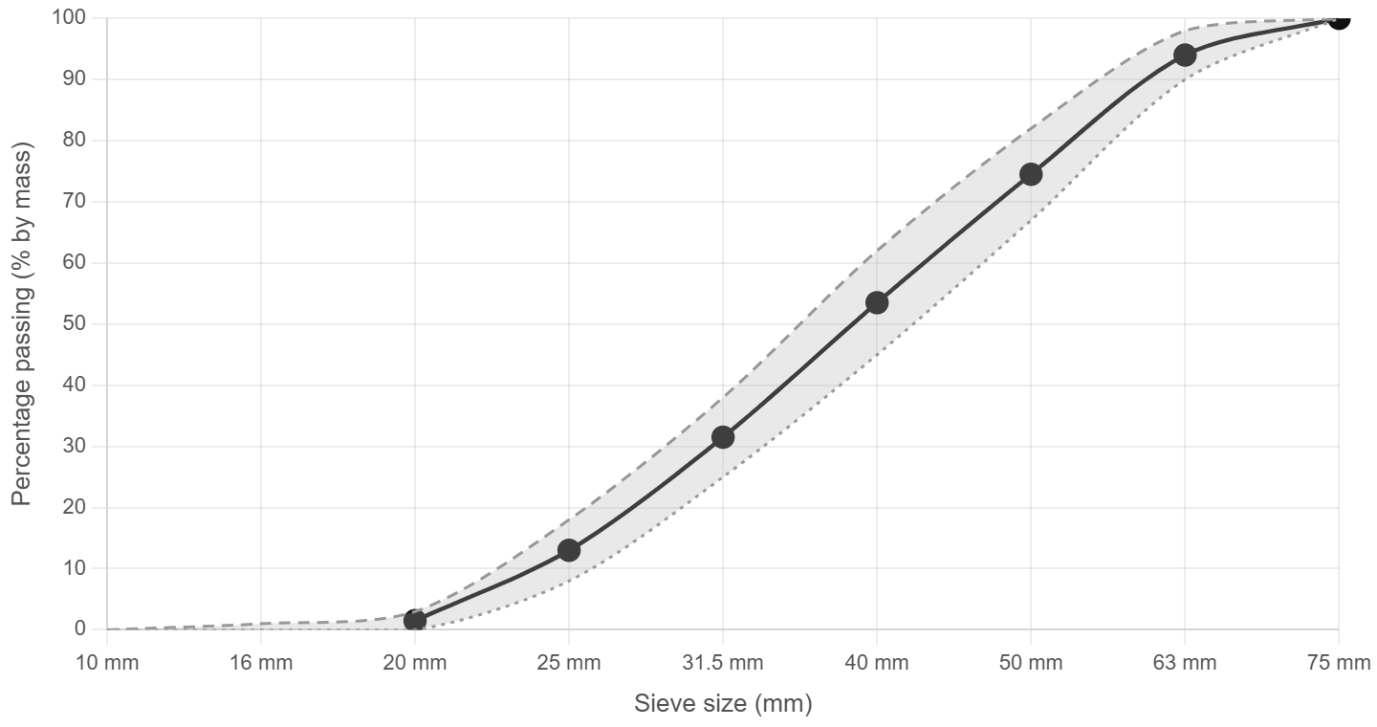
\includegraphics[width=0.85\textwidth]{image10.png}
    \caption{Pre-test particle size distribution of the basalt ballast used
             in the experimental programme, plotted against the upper and
             lower envelope curves of the \acrshort{RDSO} specification.}
    \label{fig:meth-psd}
\end{figure}

\subsection{Physical and mechanical properties}
\label{sec:meth-properties}

The ballast was characterised for the physical and mechanical properties
required by the \gls{RDSO} specification. The measurements are summarised in
\cref{tab:meth-ballast-properties}. All values fall within the \gls{RDSO}
acceptance thresholds; the \gls{AIV} measured on the artificially crushed
\SIrange{10}{12.5}{\milli\metre} sub-sample is reported here for
completeness but is precisely the index whose limitations are set out in
Chapters~\ref{chap:introduction} and~\ref{chap:literature}. The remainder of
the programme accordingly reports the bulk fouling index \FIIN{} on the
full-size specimen.

\begin{table}[ht]
\centering
\caption{Physical and mechanical properties of the basalt ballast used in
         the experimental programme.}
\label{tab:meth-ballast-properties}
\rowcolors{2}{rowbg}{white}
\begin{tabular}{@{}lccl@{}}
    \toprule
    \rowcolor{tablehdr}
    {\color{white}\textbf{Property}}
    & {\color{white}\textbf{Measured}}
    & {\color{white}\textbf{\acrshort{RDSO} limit}}
    & {\color{white}\textbf{Method}}\\
    \midrule
    Dry particle density (\si{\gram\per\centi\metre\cubed})
        & 2.78 & \(\ge 2.60\) & Gas pycnometer $+$ weighing\\
    Bulk (loose) density (\si{\kilogram\per\metre\cubed})
        & 1460 & Not specified & Bulk volume in mould\\
    Water absorption (\si{\percent})
        & 0.72 & \(\le 1.0\) & ASTM~C127 equivalent\\
    \acrshort{AAV} (\acrshort{LAA}) (\si{\percent})
        & 15.4 & \(\le 30\) & IS:2386 Pt~IV\\
    \acrshort{AIV} (\si{\percent})
        & 12.1 & \(\le 20\) & IS:2386 Pt~IV (conventional)\\
    \bottomrule
\end{tabular}
\end{table}

\begin{figure}[ht]
    \centering
    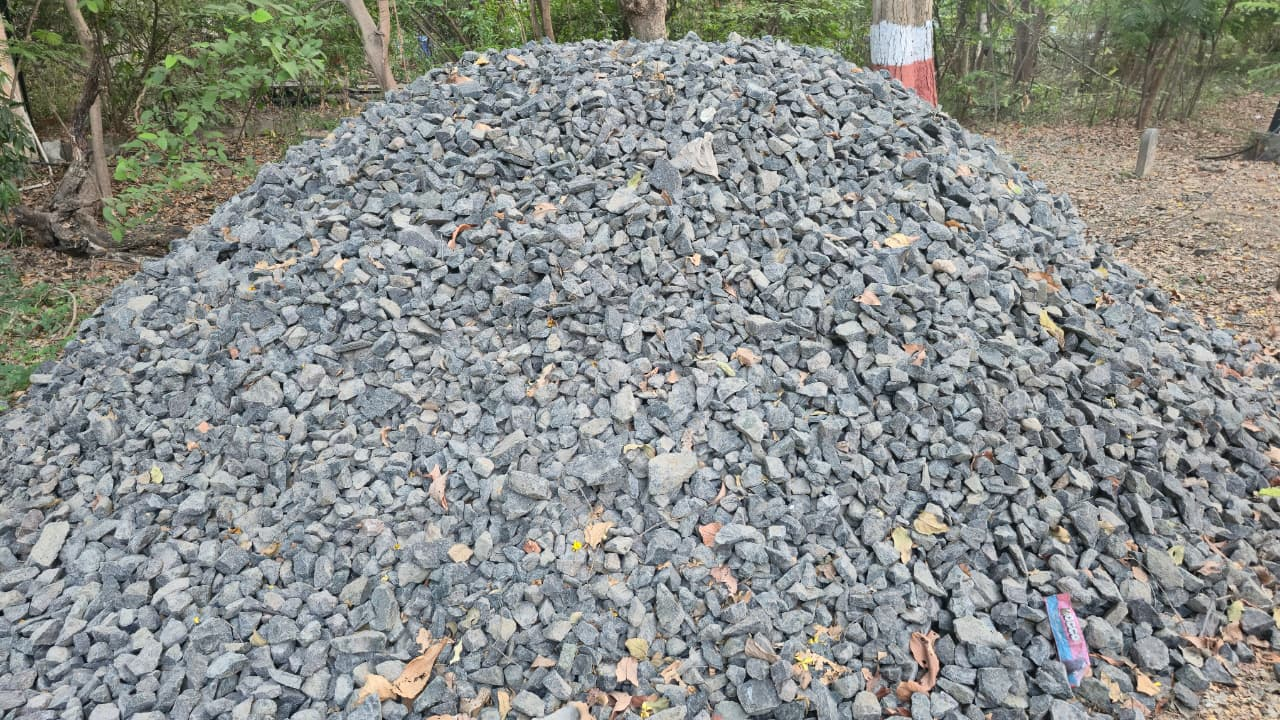
\includegraphics[width=0.70\textwidth]{image11.jpeg}
    \caption{Pile of the \acrshort{RDSO}-gradation basalt ballast used in
             the experimental programme (Civil Lab, \acrshort{GSV}).}
    \label{fig:meth-ballast-pile}
\end{figure}

\section{Reinforcement Conditions}
\label{sec:meth-reinforcement}

Three pad conditions and two base conditions are crossed in the factorial
test matrix. The three pad conditions are an Unreinforced (\gls{UR})
control, a Rubber Under-Ballast Mat (\gls{RUBM}), and a Polyurethane
Under-Ballast Mat (\gls{PUBM}). The two base conditions are a Flexible Base
(\gls{FB}) of compacted sand and a Rigid Base (\gls{RB}) of the concrete
mould floor. The systematic three-letter abbreviations are introduced
formally in this thesis as a replacement for the ad-hoc numbered test
labels used in earlier laboratory work.

\subsection{Unreinforced (UR) control}
\label{sec:meth-UR}

The \gls{UR} configuration places no pad between the ballast fill and the
base element of the mould. The \gls{UR} condition serves three analytical
purposes simultaneously: it is the mechanical control against which the two
pad conditions are compared; it represents the in-service condition of
legacy ballasted track with no substructure reinforcement; and it isolates
the effect of the base condition (flexible sand versus rigid concrete) from
the effect of any compliant pad placed above it. The \gls{UR} condition is
present in three of the nine test configurations, providing the baseline
against which the pad-protected configurations are measured.

\subsection{Rubber Under-Ballast Mat (RUBM)}
\label{sec:meth-RUBM}

The \gls{RUBM} material is a commercially manufactured \SI{12}{\milli\metre}
thick sheet of vulcanised natural rubber with a Shore~A hardness of
approximately~65 and a nominal bulk density of
\SI{1.35}{\gram\per\centi\metre\cubed}. The sheet was cut to a circular disc
matching the \SI{300}{\milli\metre} internal diameter of the test mould and
placed flat on the base element before the ballast fill. The compliance of
the \gls{RUBM} falls in the middle of the range reported in the literature
for natural-rubber under-ballast mats
\citep{Navaratnarajah2017, Ngo2019}---sufficient to dissipate a meaningful
fraction of the hammer impulse energy while stiff enough to recover
elastically between blows without progressive plastic deformation of the pad
itself. No \gls{RUBM} specimen was reused between tests; a fresh
\SI{12}{\milli\metre} disc was cut for every test to eliminate any
carry-over effect of cumulative pad damage.

\begin{figure}[ht]
    \centering
    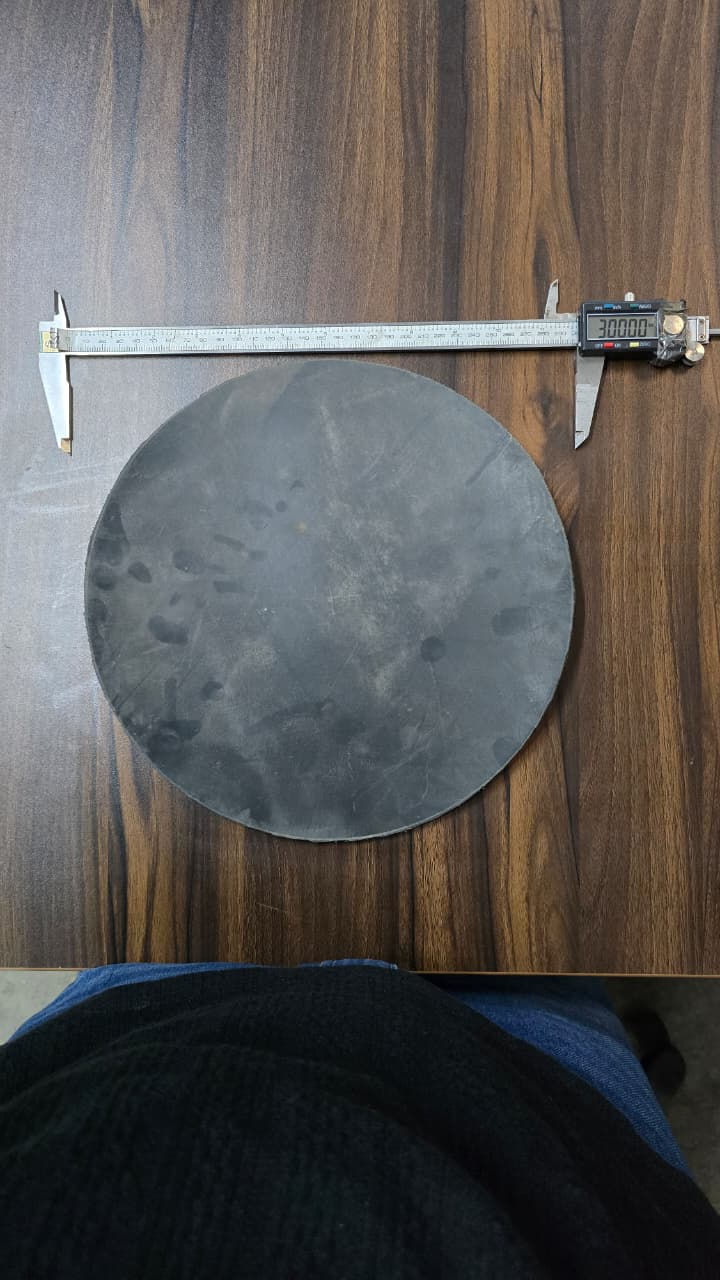
\includegraphics[width=0.55\textwidth]{image12.jpeg}
    \caption{Rubber Under-Ballast Mat (\acrshort{RUBM}) disc,
             \SI{12}{\milli\metre} thick natural rubber, cut to
             \SI{300}{\milli\metre} diameter.}
    \label{fig:meth-RUBM}
\end{figure}

\subsection{Polyurethane Under-Ballast Mat (PUBM)}
\label{sec:meth-PUBM}

The \gls{PUBM} material is a commercial Getzner polyurethane under-ballast
mat product. Getzner is a widely adopted supplier of polyurethane
track-resilient elements on European, Australian, and Indian mainline and
urban rail networks, and the specific variant used in this study is
representative of the stiffness range in which Getzner UBM products are
typically deployed beneath ballast in transition zones and impact-prone
locations. The \gls{PUBM} disc was cut to \SI{300}{\milli\metre} diameter
matching the mould internal diameter, like the \gls{RUBM}. \citet{Gundavaram2023}
have previously demonstrated, in cyclic-triaxial tests on Indian ballast,
that an elastomeric polyurethane inclusion materially reduces both
cumulative plastic deformation and the rate of fines generation, and the
use of \gls{PUBM} in the present programme extends that line of evidence
from cyclic to impact loading.

\begin{figure}[ht]
    \centering
    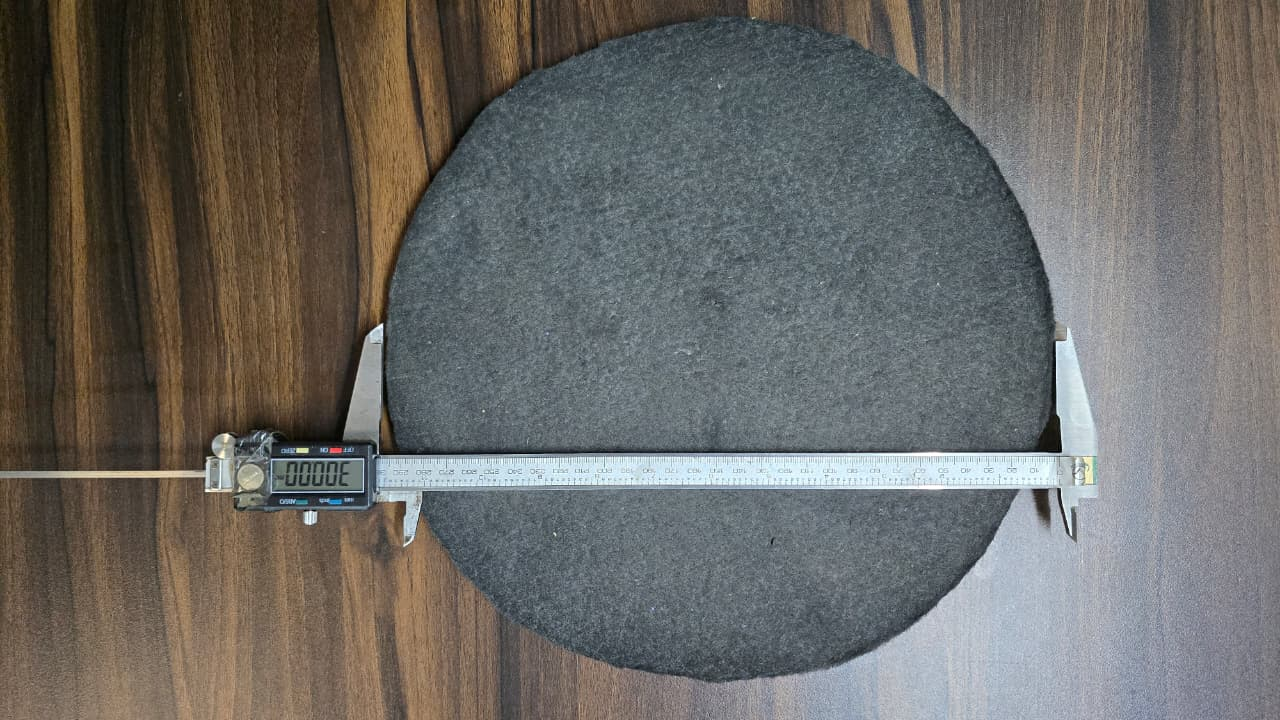
\includegraphics[width=0.55\textwidth]{image13.jpeg}
    \caption{Polyurethane Under-Ballast Mat (\acrshort{PUBM}, commercial
             Getzner product), cut to \SI{300}{\milli\metre} diameter.}
    \label{fig:meth-PUBM}
\end{figure}

\subsection{Base conditions (FB / RB)}
\label{sec:meth-base}

The base condition---the element directly beneath the pad, or beneath the
ballast if no pad is used---is the second factorial variable in the
experimental design. The \gls{FB} condition comprises a
\SI{100}{\milli\metre} deep cushion of clean, medium-grained quartz sand
placed at the base of the test mould before the pad and ballast fill. The
sand was oven-dried to constant mass and compacted in the mould by a
standardised vibratory compaction protocol to a bulk density of
approximately \SI{1.60}{\gram\per\centi\metre\cubed}. The \gls{RB}
condition places the ballast fill (with or without the interposed pad)
directly on the concrete floor of the test mould. The concrete floor is
several orders of magnitude stiffer than either the pad or the sand base
and is effectively unyielding at the stress levels delivered by the hammer.

The two base conditions are chosen to bracket the stiffness range that a
ballast layer might encounter in service: the \gls{FB} approximates a
well-compacted granular sub-ballast, while the \gls{RB} approximates an
unyielding structural element such as a bridge deck, a concrete track-slab
foundation, or a poorly-maintained subgrade that has densified below its
own elastic limit. The factorial crossing of pad and base conditions allows
the pad-effect contribution and the base-effect contribution to be
separated cleanly, which is the analytical design that \citet{Nimbalkar2012}
identified as essential for distinguishing pad performance from sub-grade
compliance in laboratory shock-mat work.

\begin{figure}[ht]
    \centering
    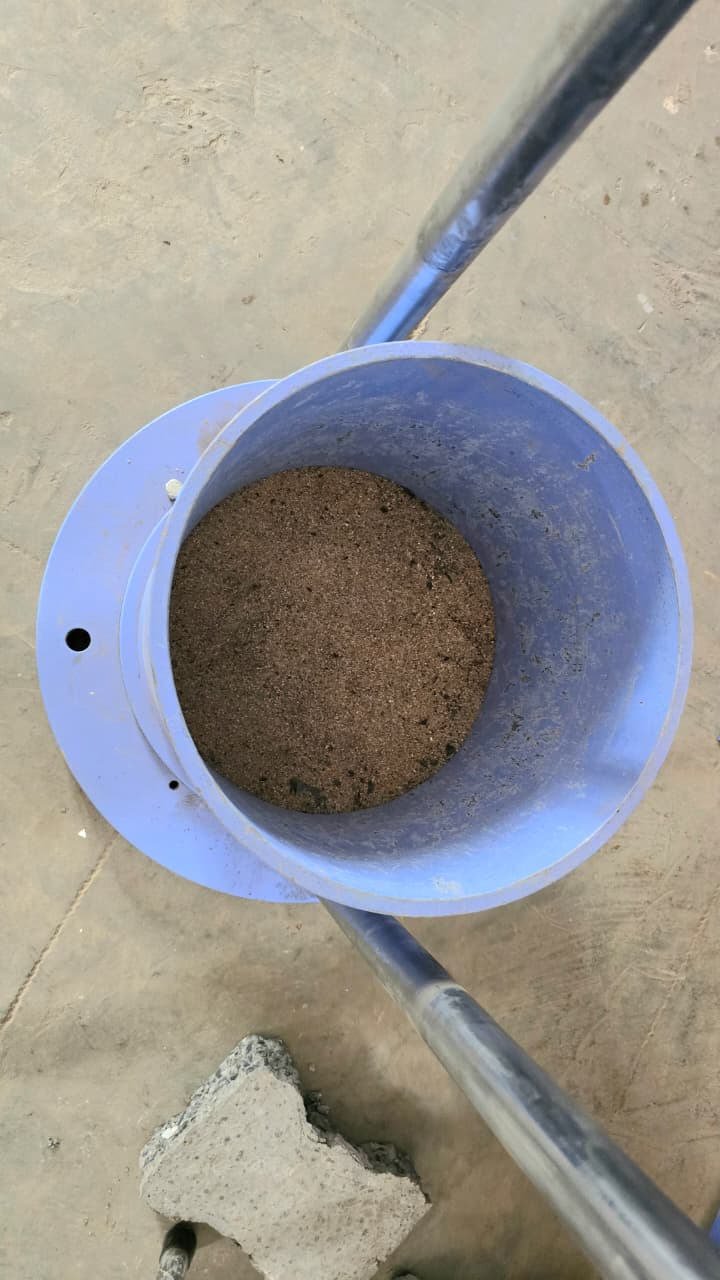
\includegraphics[width=0.55\textwidth]{image14.jpeg}
    \caption{Test mould prepared with the \SI{100}{\milli\metre} flexible
             base sand cushion (\acrshort{FB} condition), photographed
             immediately before placement of the pad and the ballast fill.}
    \label{fig:meth-FB}
\end{figure}

\section{Particle scanning}
\label{sec:meth-scanning}

\subsection{Rationale for the paired-particle design}
\label{sec:meth-paired-rationale}

The thesis rests on a paired-particle experimental design: the same physical
grains are scanned before and after the impact-loading event, and the
grain-scale damage is tracked within each particle rather than averaged
across the population.

\begin{mechanism}[title=Why pair before and after?]
Pairing eliminates the particle-to-particle variability in initial shape
---which in any typical ballast assembly is considerable, with volumes
ranging over almost an order of magnitude across the
\SIrange{20}{65}{\milli\metre} gradation---as a source of scatter in the
damage signal. It also enables the direct attribution of each observed
change in shape descriptors to the loading event, because any change
recorded in the after-scan that is not also present in the before-scan of
the same particle must have arisen from the hammer blows.
\end{mechanism}

\subsection{Selection criteria}
\label{sec:meth-selection}

Tracer particles were selected from the bulk stockpile by visual inspection
and by calliper measurement. Four criteria were applied in sequence; a
candidate particle had to satisfy all four to be accepted as a tracer.

\begin{enumerate}[label=(\roman*),leftmargin=*]
    \item \textbf{Size:} the equivalent spherical diameter---estimated at
          the selection stage from the three calliper-measured principal
          dimensions---had to fall in the
          \SIrange{30}{65}{\milli\metre} range.
    \item \textbf{Shape:} particles with extreme flatness or elongation
          (aspect ratio $L/S>3$ by initial calliper reading) were rejected
          because such shapes produce preferentially high breakage under
          impact loading and would distort the \gls{ModeA} / \gls{ModeB}
          distribution.
    \item \textbf{Parent freshness:} candidates showing any visible
          weathering rind, iron-oxide staining, or surface cementation were
          rejected.
    \item \textbf{Identifiability:} the selected particles had to admit a
          unique, durable surface marking for unambiguous before--after
          pairing.
\end{enumerate}

Each selected tracer particle was individually marked with a unique code.
The marking protocol uses a paint marker applied to a clean, dry surface
patch on each particle. The paint coat is thin
(\(<\SI{0.2}{\milli\metre}\)) and does not measurably affect either the
volume or the surface area computed from the scans.

\begin{figure}[ht]
    \centering
    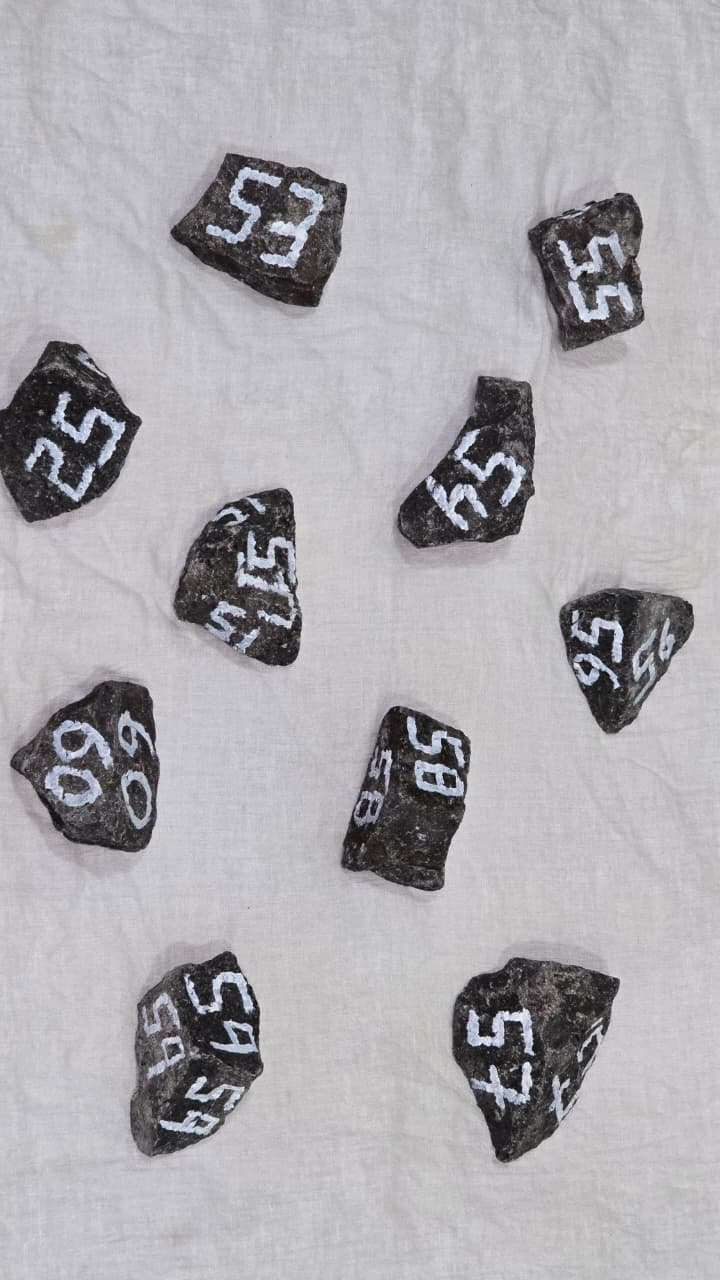
\includegraphics[width=0.65\textwidth]{image15.jpeg}
    \caption{Marked tracer particles showing the white acrylic paint patch
             and the hand-written numeric identifier code.}
    \label{fig:meth-tracers}
\end{figure}

\subsection{Pre-test structured-light scanning}
\label{sec:meth-prescan}

Each tracer particle was scanned on an EinScan (Shining 3D Technology
Co.\ Ltd., Hangzhou, China) desktop structured-light scanner. The
EinScan~SE was used across the programme, providing comparable geometric
accuracy of approximately \SI{0.1}{\milli\metre} and scan resolution of
approximately \SI{0.15}{\milli\metre} in the automatic turntable mode used
here. The detailed scan-protocol and mesh quality-control procedures are
set out in \cref{sec:meth-morphology} below, in the context of the
morphological-analysis pipeline. In the present sub-section pre-test
scanning is described as part of specimen preparation: every tracer
particle carried a complete, validated, watertight triangular surface mesh
in \gls{STL} format into the impact test, and the pre-test mesh serves as
the reference state against which the post-test mesh is paired.

\begin{figure}[ht]
    \centering
    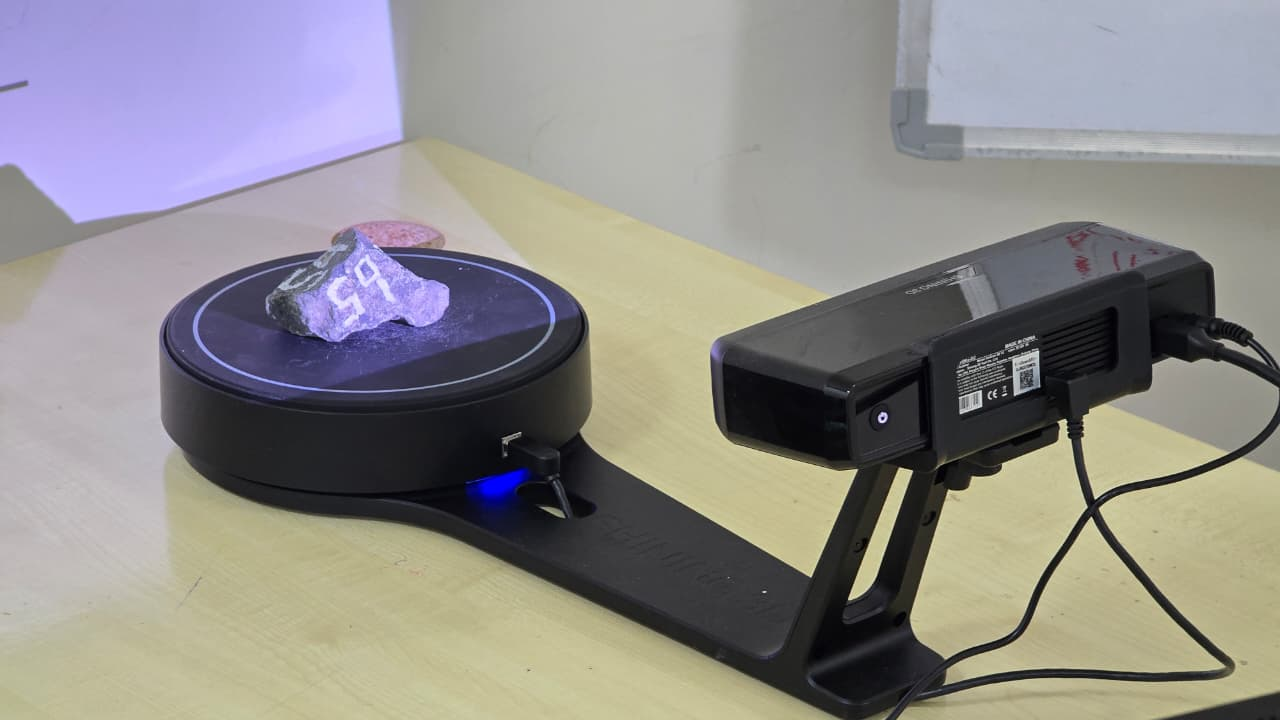
\includegraphics[width=0.65\textwidth]{image16.jpeg}
    \caption{EinScan structured-light scanner (Shining~3D) in operation with
             a marked tracer particle mounted on the automatic turntable.}
    \label{fig:meth-einscan}
\end{figure}

\section{The modified drop-weight impact apparatus}
\label{sec:meth-apparatus}

The apparatus comprises five principal components: a cylindrical cast-iron
test mould of \SI{300}{\milli\metre} internal diameter and
\SI{350}{\milli\metre} internal depth, seated on a rigid reaction
base-plate; a vertical guide frame of four mild-steel columns connected by
an upper crosshead; a cylindrical cast-iron hammer of \SI{50}{\kilogram}
mass, sliding on the guide columns in free fall; a continuously adjustable
hammer release-and-locking mechanism graduated over the
\SIrange{200}{450}{\milli\metre} range of drop height; and a load-transfer
assembly consisting of a \SI{300}{\milli\metre} bearing plate, a
compression-type \SI{5}{\tonne} strain-gauge load cell, and a hardened-steel
striker plate. A mechanical blow counter and two manual operating handles
complete the assembly. The mould diameter of \SI{300}{\milli\metre} delivers
a $D/\dmax$ ratio of approximately~6 against the \gls{RDSO}
\SI{50}{\milli\metre} mean particle size, eliminating the boundary-dominance
of the conventional IS:2386 Part~IV apparatus \citep{BIS1963} and bringing
the present rig into the design envelope established by
\citet{Nimbalkar2012} and the subsequent impact literature surveyed in
\cref{sec:lit-lab}.

The adjustable release mechanism permits the hammer to be locked at any
drop height between \SI{200}{\milli\metre} and \SI{450}{\milli\metre}
against a graduated scale on one of the four guide columns, so that the
same apparatus can deliver a range of impact energies without disassembly.
The in-line load cell measures the dynamic peak force imparted through the
striker plate on every blow and transmits the signal to a digital
peak-force indicator; this allows each test to be characterised not only by
its nominal drop-energy but by the actual force time-series, which is the
principal advance of the present rig over the conventional apparatus. The
mechanical blow counter provides a redundant and power-independent count of
delivered blows. Detailed design drawings, material specifications,
tolerance callouts, and the safety-interlock documentation are set out in
the utility patent application filed for this apparatus.

\begin{figure}[ht]
\centering
\begin{tikzpicture}[scale=0.9,>=Stealth,every node/.style={font=\footnotesize}]
    % --- Frame columns (4 guide rods) ---
    \draw[gsvblue!40,line width=1.5pt] (-3.2,-3.2) -- (-3.2,7.2);
    \draw[gsvblue!40,line width=1.5pt] ( 3.2,-3.2) -- ( 3.2,7.2);
    \node[font=\scriptsize,gsvblue,rotate=90] at (-3.7,2)
        {\bfseries Guide column (4)};

    % --- Top crosshead ---
    \fill[gsvblue!80] (-3.4, 7.0) rectangle (3.4, 7.4);
    \draw[gsvblue,thick] (-3.4, 7.0) rectangle (3.4, 7.4);
    \node[white,font=\scriptsize\bfseries] at (0,7.2) {Top crosshead};

    % --- Release / lifting mechanism ---
    \draw[gsvaccent,thick,fill=gsvaccent!20] (-0.5,6.3) rectangle (0.5,7.0);
    \node[font=\tiny,gsvaccent!80!black] at (0,6.65) {release};
    \node[font=\scriptsize,gsvblue!90!black,anchor=west]
        at (0.8,6.65) {Mechanical release latch};

    % --- Hammer (50 kg) ---
    \draw[gsvblue,thick,fill=gsvblue!85,rounded corners=2pt]
        (-1.7,4.6) rectangle (1.7,5.7);
    \node[white,font=\bfseries\small] at (0,5.15) {Hammer (50\,kg)};
    % Drop arrow
    \draw[->,line width=1.4pt,red!70] (0,4.55) -- (0,3.65)
        node[midway,right=4pt,red!80,font=\scriptsize] {drop $h$};
    % Drop-height markings
    \draw[gsvblue!50,dotted] (1.7,5.15) -- (3.3,5.15);
    \node[font=\tiny,gsvblue!70,anchor=west] at (3.3,5.15)
        {hammer release elevation};

    % --- Striker plate ---
    \draw[gray!60,thick,fill=gray!40] (-1.5,3.3) rectangle (1.5,3.55);
    \node[font=\scriptsize,gsvblue!90!black,anchor=west] at (1.7,3.43)
        {Striker plate (\SI{300}{\milli\metre})};

    % --- In-line load cell ---
    \draw[gsvaccent!80!black,thick,fill=gsvaccent!30]
        (-0.85,3.0) rectangle (0.85,3.3);
    \node[font=\tiny,gsvaccent!80!black] at (0,3.15) {load cell};
    \node[font=\scriptsize,gsvblue!90!black,anchor=west] at (1.7,3.15)
        {In-line \SI{5}{\tonne} load cell};

    % --- Bearing plate ---
    \draw[gray!60,thick,fill=gray!40] (-1.6,2.7) rectangle (1.6,3.0);
    \node[font=\scriptsize,gsvblue!90!black,anchor=west] at (1.7,2.85)
        {Bearing plate};

    % --- Mould (cylindrical specimen container) ---
    \draw[gsvblue,thick,fill=gsvblue!8]
        (-2.3,0.5) -- (-2.3,2.7) -- (-2.0,2.7) -- (-2.0,0.5)
        -- (2.0,0.5) -- (2.0,2.7) -- (2.3,2.7) -- (2.3,0.5)
        -- cycle;
    % Specimen contents -- ballast layer
    \begin{scope}[clip]
        \path (-2.0,0.9) rectangle (2.0,2.65);
    \end{scope}
    \foreach \x/\y/\r in {
        -1.6/2.4/0.16, -1.1/2.45/0.18, -0.4/2.4/0.15, 0.3/2.5/0.17, 1.0/2.4/0.16, 1.55/2.45/0.16,
        -1.7/2.0/0.18, -1.0/2.05/0.16, -0.2/2.0/0.18, 0.5/2.1/0.16, 1.2/2.0/0.17, 1.7/2.05/0.15,
        -1.5/1.6/0.17, -0.7/1.55/0.18, 0.0/1.6/0.16, 0.7/1.55/0.18, 1.4/1.6/0.16,
        -1.7/1.15/0.16, -1.0/1.2/0.17, -0.2/1.15/0.16, 0.5/1.2/0.18, 1.2/1.15/0.16, 1.7/1.2/0.15}
        \fill[gray!55] (\x,\y) circle (\r);
    \node[font=\scriptsize,gsvblue!90!black,anchor=west] at (2.6,2.0)
        {Ballast fill (20\,kg)};
    % Pad layer
    \fill[orange!50] (-2.0,0.85) rectangle (2.0,0.95);
    \node[font=\scriptsize,orange!80!black,anchor=west] at (2.6,0.9)
        {Pad (PUBM/RUBM/UR)};
    % Base layer
    \fill[gsvblue!90] (-2.0,0.55) rectangle (2.0,0.85);
    \node[font=\scriptsize,gsvblue!90!black,anchor=west] at (2.6,0.7)
        {Base (FB / RB)};

    % --- Floor / base of apparatus ---
    \fill[gray!50] (-3.4,-0.2) rectangle (3.4,0.5);
    \draw[gsvblue,thick] (-3.4,-0.2) rectangle (3.4,0.5);
    \node[white,font=\scriptsize\bfseries] at (0,0.15) {Steel base plate};

    % --- Concrete floor (hatched) ---
    \fill[gray!30,pattern=north east lines] (-3.4,-1.5) rectangle (3.4,-0.2);
    \node[font=\scriptsize,gray!50!black,anchor=west] at (-3.0,-0.85)
        {Reinforced concrete floor};

    % --- Dimensional callouts ---
    \draw[<->,gsvblue!70] (-3.6, 5.15) -- (-3.6, 3.55)
        node[midway,left,gsvblue,font=\scriptsize,align=right]
        {200--450\,mm\\drop range};

    % --- Digital indicator ---
    \draw[gsvblue,thick,fill=white]
        (3.9, 4.0) rectangle (5.1, 5.0);
    \node[font=\scriptsize\bfseries,gsvblue] at (4.5, 4.7) {LCD};
    \node[font=\tiny,red!80,font=\ttfamily] at (4.5, 4.4) {37.0\,kN};
    \node[font=\tiny,gsvblue] at (4.5, 4.15) {peak force};
    \draw[->,gsvblue!60,thick] (3.6, 3.15) -- (3.9, 4.0);
\end{tikzpicture}
\caption{Schematic of the modified large-scale drop-weight impact
         apparatus. The hammer (\SI{50}{\kilogram}) is locked at a
         release elevation between \SI{200}{\milli\metre} and
         \SI{450}{\milli\metre} above the striker plate. The in-line
         \SI{5}{\tonne} load cell records the peak contact force at
         every blow and displays the value on the LCD indicator (right).
         The specimen mould holds the layered base, pad, and
         \SI{20}{\kilogram} ballast fill. Four guide columns ensure
         vertical impact alignment.}
\label{fig:meth-apparatus-schematic}
\end{figure}

\begin{figure}[ht]
    \centering
    \begin{subfigure}{0.46\textwidth}
        \centering
        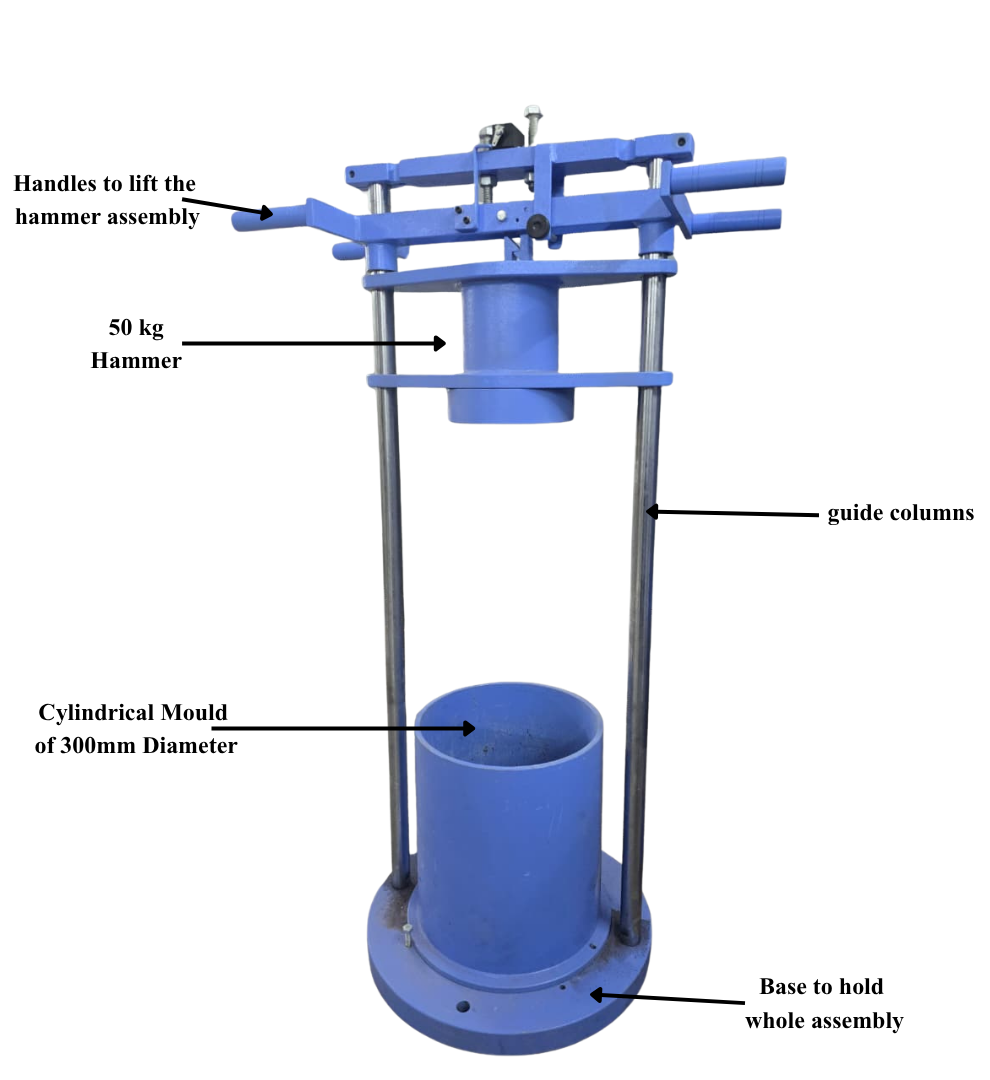
\includegraphics[width=\linewidth]{image17.png}
        \caption{Full apparatus view.}
    \end{subfigure}\hfill
    \begin{subfigure}{0.46\textwidth}
        \centering
        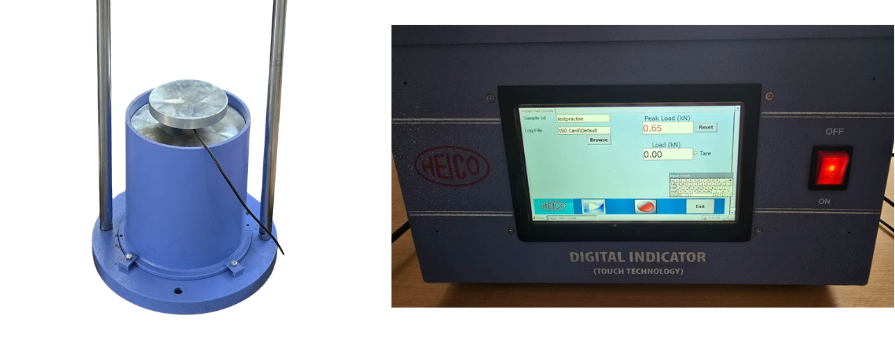
\includegraphics[width=\linewidth]{image18.png}
        \caption{Load-transfer assembly.}
    \end{subfigure}
    \caption{Modified drop-weight impact apparatus (photographs
             matching Figure~\ref{fig:meth-apparatus-schematic}). (a)
             Overall view of the apparatus and its frame. (b) Close-up
             of the load-transfer assembly (bearing plate,
             \SI{5}{\tonne} load cell, striker plate) and the digital
             peak-force display.}
    \label{fig:meth-apparatus}
\end{figure}

\subsection{Comparison with the conventional AIV apparatus}
\label{sec:meth-AIV-comparison}

The salient design differences between the conventional IS:2386 Part~IV
\gls{AIV} apparatus and the modified large-scale apparatus commissioned at
\gls{GSV} are tabulated in \cref{tab:meth-AIV-comparison}.

\begin{table}[ht]
\centering
\caption{Principal specification of the modified apparatus in comparison to
         the conventional IS:2386 Part~IV Aggregate Impact Value apparatus.
         Only the headline parameters are listed; the full specification is
         in the patent documentation (\cref{chap:appB}).}
\label{tab:meth-AIV-comparison}
\small
\rowcolors{2}{rowbg}{white}
\begin{adjustbox}{max width=\textwidth}
\begin{tabular}{@{}p{4.4cm}p{4.8cm}p{5.6cm}@{}}
    \toprule
    \rowcolor{tablehdr}
    {\color{white}\textbf{Parameter}}
    & {\color{white}\textbf{Conventional \acrshort{AIV} (IS:2386 Pt~IV)}}
    & {\color{white}\textbf{Modified apparatus (present)}}\\
    \midrule
    Mould internal diameter
        & \SI{102}{\milli\metre} & \SI{300}{\milli\metre}\\
    Mould effective depth
        & \(\sim\!\SI{50}{\milli\metre}\) & \SI{350}{\milli\metre}\\
    Hammer mass
        & \SI{13.5}{\kilogram} & \SI{50}{\kilogram}\\
    Drop height
        & \SI{380}{\milli\metre} (fixed)
        & \SIrange{200}{450}{\milli\metre} (adjustable)\\
    Particle size tested
        & \SIrange{10}{12.5}{\milli\metre} (crushed sub-sample)
        & \SIrange{20}{63}{\milli\metre} (full \acrshort{RDSO} gradation)\\
    Approx.\ particles per test
        & \numrange{2}{4} & \numrange{40}{80}\\
    $D/\dmax$ ratio
        & \(\approx 1.6\) (boundary-dominated)
        & \(\approx 6\) (boundary-free)\\
    Stress simulation
        & Fixed / none
        & \SIrange{275}{523}{\kilo\pascal} (adjustable, maps to
        \SI{22.5}{\tonne} axle)\\
    Real-time force measurement
        & None
        & \SI{5}{\tonne} load cell $+$ digital peak-force indicator\\
    Blow counting
        & Manual & Integrated mechanical counter\\
    Post-test degradation metric
        & \acrshort{AIV} (\(\%\) fines through \SI{2.36}{\milli\metre})
        & \FIIN{} $+$ paired per-particle morphology\\
    \bottomrule
\end{tabular}
\end{adjustbox}
\end{table}

\section{Stress and energy calibration to Indian Railways field loading}
\label{sec:meth-calibration}

The calibration of the apparatus to in-service stress conditions proceeds
in two steps: first, the in-service stress range at the top of the ballast
layer under Indian Railways axle loading is estimated; second, the hammer
mass and drop-height range of the apparatus are chosen to span this
in-service range when divided by the mould cross-sectional area.

\subsection{Field stress estimation}
\label{sec:meth-field-stress}

The wheel load is distributed through the rail to the sleeper beneath it,
and thence to the ballast over the effective sleeper--ballast bearing area.
For a pre-stressed concrete mainline sleeper on Indian Railways the
effective bearing area is approximately
\SIrange{2000}{2200}{\centi\metre\squared}, of which the two rail-seat
regions each carry roughly half the axle load on each rail. Taking $\Ab
\approx \SI{1100}{\centi\metre\squared}$ as the effective bearing area
below a single rail seat, the static contact stress at the top of the
ballast under a \SI{22.5}{\tonne} axle is
\begin{equation}
    \sigma_{\text{static}} = \frac{W}{\Ab}
    \approx \frac{\SI{110.25}{\kilo\newton}}{\SI{0.11}{\metre\squared}}
    \approx \SI{1000}{\kilo\newton\per\metre\squared}
    \approx \SI{250}{\kilo\pascal}.
    \label{eq:meth-sigma-static}
\end{equation}
Applying a conservative dynamic amplification of~1.5 under ordinary
mainline traffic yields $\sigma \approx \SI{375}{\kilo\pascal}$; at
impact-prone locations where the amplification can reach $2\times$ or
higher, the contact stress rises into the
\SIrange{500}{600}{\kilo\pascal} range. The in-service stress window at the
top of the ballast layer under Indian Railways traffic is therefore
conservatively taken as approximately \SIrange{250}{550}{\kilo\pascal},
with the upper end reflecting heavy-haul and transition-zone conditions.

\subsection{Apparatus stress and energy}
\label{sec:meth-apparatus-stress}

For the modified apparatus the nominal contact stress $\sigma$ is the peak
hammer force $F$ divided by the bearing-plate area $\Ap$. The hammer
kinetic energy at impact is
\begin{equation}
    \Ke = m\,g\,h,
    \label{eq:meth-ke}
\end{equation}
where $m$ is the hammer mass (\SI{50}{\kilogram}), $g$ is the gravitational
acceleration (\SI{9.81}{\metre\per\second\squared}), and $h$ is the drop
height. Using the measured peak forces reported at commissioning---$F
\approx \SI{19.4}{\kilo\newton}$ at $h = \SI{300}{\milli\metre}$ and $F
\approx \SI{37.0}{\kilo\newton}$ at $h = \SI{450}{\milli\metre}$---and the
bearing-plate area $\Ap = \pi\,(\SI{0.150}{\metre})^{2} =
\SI{0.0707}{\metre\squared}$, the two apparatus operating points correspond
to
\begin{align}
    h &= \SI{300}{\milli\metre}: &
    \Ke &= 50 \times 9.81 \times 0.300 = \SI{147}{\joule}, &
    \sigma &= \frac{\SI{19.4}{\kilo\newton}}{\SI{0.0707}{\metre\squared}}
        \approx \SI{275}{\kilo\pascal};
        \label{eq:meth-h300}\\
    h &= \SI{450}{\milli\metre}: &
    \Ke &= 50 \times 9.81 \times 0.450 = \SI{221}{\joule}, &
    \sigma &= \frac{\SI{37.0}{\kilo\newton}}{\SI{0.0707}{\metre\squared}}
        \approx \SI{523}{\kilo\pascal}.
        \label{eq:meth-h450}
\end{align}

\begin{finding}[title=Calibration outcome]
The two operating points---\SI{275}{\kilo\pascal} at \SI{147}{\joule} and
\SI{523}{\kilo\pascal} at \SI{221}{\joule}---correspond respectively to the
lower end (ordinary mainline traffic) and the upper end (heavy-haul and
transition-zone conditions) of the in-service stress window. The two drop
heights selected for the test programme therefore bracket the Indian
Railways field-loading envelope cleanly.
\end{finding}

\begin{figure}[ht]
\centering
\begin{tikzpicture}[>=Stealth,every node/.style={font=\footnotesize}]
    % Vertical stress axis
    \draw[thick,->] (0,0) -- (0,7.2) node[above]
        {\scriptsize $\sigma$ (\si{\kilo\pascal})};
    \foreach \y/\v in {0.5/250,1.5/300,2.5/350,3.5/400,4.5/450,5.5/500,6.5/550}
        \draw (-0.1,\y) -- (0.1,\y) node[left,xshift=-0.15cm] {\v};

    % Field stress band
    \fill[gsvblue!15] (0.7, 0.5) rectangle (4.5, 6.5);
    \node[gsvblue,align=center] at (2.6, 3.5)
        {In-service stress\\window\\\textbf{250--550 \si{\kilo\pascal}}};
    \node[gsvblue,anchor=west,font=\scriptsize\itshape] at (0.7, 0.3)
        {static \SI{250}{\kilo\pascal}};
    \node[gsvblue,anchor=west,font=\scriptsize\itshape] at (0.7, 6.7)
        {impact-zone \SI{550}{\kilo\pascal}};

    % Apparatus operating points
    \draw[->,thick,boxmech!80] (5.6, 0.75) -- (4.5, 0.75);
    \node[fill=boxmech,text=white,rounded corners=2pt,
          font=\small\bfseries] at (6.2, 0.75)
        {\SI{300}{\milli\metre} drop};
    \node[anchor=west,font=\footnotesize] at (7.2, 0.75)
        {$\sigma\approx\SI{275}{\kilo\pascal}$,\ $\Ke=\SI{147}{\joule}$};

    \draw[->,thick,boxmech!80] (5.6, 5.7) -- (4.5, 5.7);
    \node[fill=boxmech,text=white,rounded corners=2pt,
          font=\small\bfseries] at (6.2, 5.7)
        {\SI{450}{\milli\metre} drop};
    \node[anchor=west,font=\footnotesize] at (7.2, 5.7)
        {$\sigma\approx\SI{523}{\kilo\pascal}$,\ $\Ke=\SI{221}{\joule}$};

    % Brace showing apparatus range
    \draw[decorate,decoration={brace,amplitude=6pt},gsvaccent,thick]
        (5.0,0.75) -- (5.0,5.7)
        node[midway,xshift=-0.4cm,rotate=90,font=\footnotesize\bfseries,
             text=gsvaccent] {Apparatus};
\end{tikzpicture}
\caption{Apparatus calibration to the Indian Railways field-loading
         envelope. The two drop heights span the in-service stress
         window from ordinary mainline traffic
         (\(\sim\!\SI{275}{\kilo\pascal}\), \SI{147}{\joule}) to
         heavy-haul / transition-zone conditions
         (\(\sim\!\SI{523}{\kilo\pascal}\), \SI{221}{\joule}).}
\label{fig:meth-calibration-ladder}
\end{figure}

The adjustability of the drop-height mechanism over the full
\SIrange{200}{450}{\milli\metre} range leaves open the possibility of finer
calibration to specific axle-load classes in future work.

\section{Sample preparation and test protocol}
\label{sec:meth-protocol}

\subsection{Specimen assembly}
\label{sec:meth-assembly}

The nine test specimens were assembled using a single standardised
protocol that produces reproducible specimens across the three pad
conditions and the two base conditions. The protocol comprises eleven
discrete steps, summarised here in the order of execution:
\begin{enumerate}[leftmargin=*,itemsep=2pt]
    \item Inspection and cleaning of the cylindrical test mould.
    \item Base preparation.
    \item Pad placement, where applicable, with fresh discs cut for every
          test.
    \item Tracer-particle placement at pre-assigned positions in the
          lower-middle of the ballast fill, with no tracer-to-tracer or
          tracer-to-wall direct contacts.
    \item Bulk-fill placement of the remainder of the \SI{20}{\kilogram}
          specimen mass in two lifts.
    \item Final levelling of the top surface with the load-transfer
          bearing-plate verification.
    \item Load-cell zeroing and digital-indicator verification.
    \item Photographic baseline record.
    \item Hammer positioning and locking at the specified drop height.
    \item Blow delivery.
    \item Test termination, tracer recovery, and bulk-fill collection for
          sieve analysis.
\end{enumerate}

\begin{figure}[ht]
    \centering
    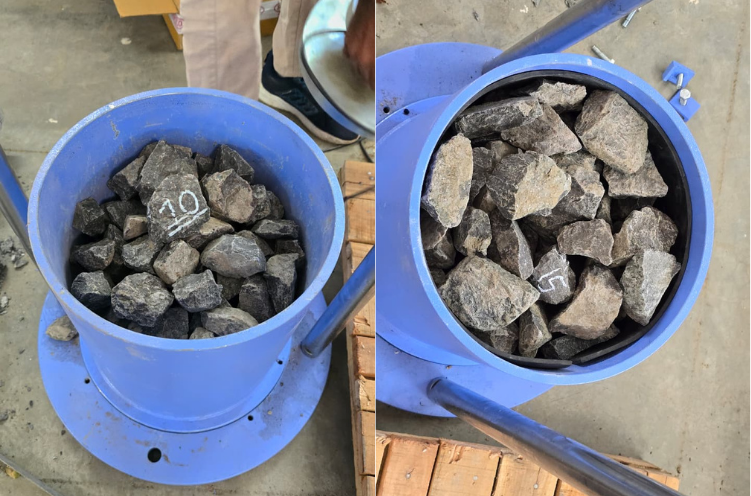
\includegraphics[width=0.55\textwidth]{image19.png}
    \caption{Assembling the test specimen in the mould (photograph without
             load-cell assembly).}
    \label{fig:meth-assembly}
\end{figure}

\subsection{Blow-by-blow test protocol}
\label{sec:meth-blow-protocol}

Each of the nine tests was conducted using an identical blow-by-blow
protocol. Twenty (20) free-fall blows were delivered per test from the
nominated drop height (either \SI{300}{\milli\metre} or
\SI{450}{\milli\metre}). The choice of 20 blows is guided by two
considerations. First, it is consistent with the number of blows used in
comparable published drop-weight studies on ballast
\citep{Nimbalkar2012, Koohmishi2020, Zhang2023}. Second, preliminary trials
showed that the settlement--blow curve flattens substantially between
blow~15 and blow~20 and enters a near-stable zone beyond blow~15; twenty
blows therefore captures both the transient settlement regime and the
early approach to the steady state.

The twenty blows were delivered in rapid succession, with an interval of
\SIrange{5}{8}{\second} between consecutive blows---long enough for the
operators to safely re-raise and re-lock the hammer, and to record the
peak-force reading, but short enough that cumulative heating of the rubber
or polyurethane pad is negligible. The hammer release was triggered by
two-operator manual action at the upper crosshead. After each blow the
hammer was secured at the crosshead before the peak-force value was read.
Axial settlement was measured at five blow milestones ($N=0, 5, 10, 15,
20$) with a depth gauge seated on the mould rim. The digital peak-force
indicator was observed and recorded for each test.

\subsection{Test matrix and nomenclature}
\label{sec:meth-matrix}

The nine test configurations are defined by the factorial crossing of the
three pad conditions (\gls{UR} / \gls{RUBM} / \gls{PUBM}), the two base
conditions (\gls{FB} / \gls{RB}), and the two impact energies
(\SI{300}{\milli\metre} and \SI{450}{\milli\metre} drop heights of the
\SI{50}{\kilogram} hammer, corresponding to nominal contact stresses of
\SI{275}{\kilo\pascal} and \SI{523}{\kilo\pascal} as derived in
\cref{sec:meth-calibration}). The nine cells listed in
\cref{tab:meth-matrix} cover the factorial with the three
\gls{FB}--\SI{450}{\milli\metre} combinations omitted because the apparatus
commissioning revealed that at the \SI{450}{\milli\metre} drop height the
sand cushion under the \gls{FB} condition would progressively lose bearing
capacity through cumulative compaction over twenty blows and would thereby
confound the pad-effect signal with a base-consolidation signal.

\begin{figure}[ht]
\centering
\begin{tikzpicture}[node distance=0.15cm,>=Stealth]
    % Column header row
    \node[labelrow] (hdr-fb300) at (0, 2.4)
        {FB -- \SI{300}{\milli\metre}\\\footnotesize\SI{275}{\kilo\pascal}, \SI{147}{\joule}};
    \node[labelrow] (hdr-rb300) at (3.4, 2.4)
        {RB -- \SI{300}{\milli\metre}\\\footnotesize\SI{275}{\kilo\pascal}, \SI{147}{\joule}};
    \node[labelrow] (hdr-rb450) at (6.8, 2.4)
        {RB -- \SI{450}{\milli\metre}\\\footnotesize\SI{523}{\kilo\pascal}, \SI{221}{\joule}};

    % Row labels
    \node[labelrow,anchor=east] (lbl-pubm) at (-1.7, 1.2) {PUBM};
    \node[labelrow,anchor=east] (lbl-rubm) at (-1.7, 0.0) {RUBM};
    \node[labelrow,anchor=east] (lbl-ur)   at (-1.7,-1.2) {UR};

    % Row 1: PUBM (green)
    \node[cellpubm] at (0, 1.2)   {\testlabel{T1}\\PUBM--FB--300};
    \node[cellpubm] at (3.4, 1.2) {\testlabel{T9}\\PUBM--RB--300};
    \node[cellpubm] at (6.8, 1.2) {\testlabel{T6}\\PUBM--RB--450};
    % Row 2: RUBM (orange)
    \node[cellrubm] at (0, 0.0)   {\testlabel{T2}\\RUBM--FB--300};
    \node[cellrubm] at (3.4, 0.0) {\testlabel{T8}\\RUBM--RB--300};
    \node[cellrubm] at (6.8, 0.0) {\testlabel{T5}\\RUBM--RB--450};
    % Row 3: UR (red)
    \node[cellur] at (0,  -1.2) {\testlabel{T3}\\UR--FB--300};
    \node[cellur] at (3.4,-1.2) {\testlabel{T4}\\UR--RB--300};
    \node[cellur] at (6.8,-1.2) {\testlabel{T7}\\UR--RB--450};
\end{tikzpicture}
\caption{The nine-cell factorial test matrix. Rows are pad conditions
         (\gls{PUBM} / \gls{RUBM} / \gls{UR}); columns are
         base--energy combinations. The three
         \gls{FB}--\SI{450}{\milli\metre} cells are excluded by design
         because the sand cushion would progressively lose bearing
         capacity at the higher drop energy (see text).}
\label{fig:meth-matrix}
\end{figure}

\begin{table}[ht]
\centering
\caption{The nine test configurations of the experimental programme.
         Systematic labels are \texttt{PAD--BASE--DROP}; the legacy
         laboratory labels (\acrshort{LH}, \acrshort{HH}) are listed for
         cross-reference with the raw laboratory records.}
\label{tab:meth-matrix}
\rowcolors{2}{rowbg}{white}
\begin{tabular}{@{}cclcccc@{}}
    \toprule
    \rowcolor{tablehdr}
    {\color{white}\textbf{Test}}
    & {\color{white}\textbf{Systematic label}}
    & {\color{white}\textbf{Legacy label}}
    & {\color{white}$\boldsymbol{h}$~(\si{\milli\metre})}
    & {\color{white}$\boldsymbol{\sigma}$~(\si{\kilo\pascal})}
    & {\color{white}$\boldsymbol{\Ke}$~(\si{\joule})}
    & {\color{white}\textbf{Peak~$F$~(\si{\kilo\newton})}}\\
    \midrule
    \testlabel{T1} & PUBM--FB--300 & PUBM-FB-LH & 300 & 275 & 147 & 19.4\\
    \testlabel{T2} & RUBM--FB--300 & RUBM-FB-LH & 300 & 275 & 147 & 19.4\\
    \testlabel{T3} & UR--FB--300   & UR-FB-LH   & 300 & 275 & 147 & 19.4\\
    \testlabel{T4} & UR--RB--300   & UR-RB-LH   & 300 & 275 & 147 & 19.4\\
    \testlabel{T5} & RUBM--RB--450 & RUBM-RB-HH & 450 & 523 & 221 & 37.0\\
    \testlabel{T6} & PUBM--RB--450 & PUBM-RB-HH & 450 & 523 & 221 & 37.0\\
    \testlabel{T7} & UR--RB--450   & UR-RB-HH   & 450 & 523 & 221 & 37.0\\
    \testlabel{T8} & RUBM--RB--300 & RUBM-RB-LH & 300 & 275 & 147 & 19.4\\
    \testlabel{T9} & PUBM--RB--300 & PUBM-RB-LH & 300 & 275 & 147 & 19.4\\
    \bottomrule
\end{tabular}
\end{table}

\subsection{Post-test sieve analysis}
\label{sec:meth-sieve}

At the end of each test the full bulk fill, together with any fines
recovered from the mould floor after tracer extraction, was sieved through
the same sieve series used for the pre-test gradation characterisation
(63, 50, 40, 31.5, 25, 20, 16, 12.5, 10, 4.75, 2.36, 0.6, 0.15 and
\SI{0.075}{\milli\metre}).

\begin{figure}[ht]
    \centering
    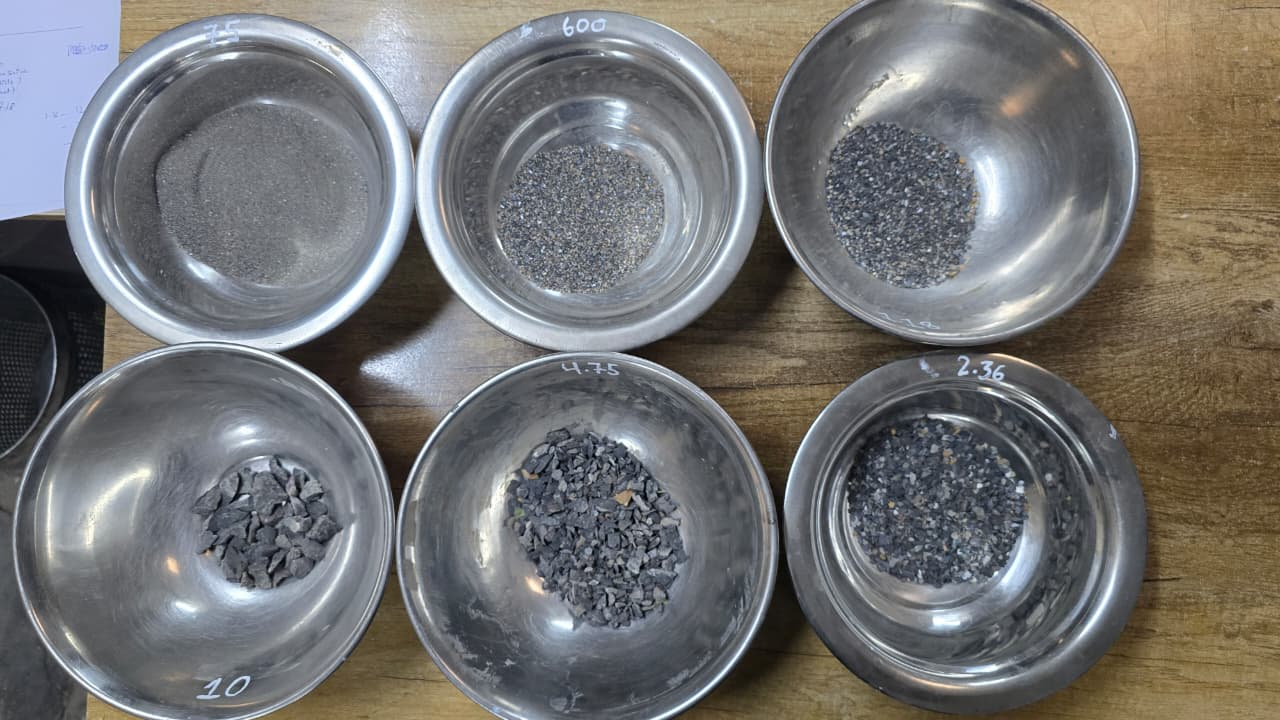
\includegraphics[width=0.55\textwidth]{image20.jpeg}
    \caption{Post-impact-test sieve analysis.}
    \label{fig:meth-sieve}
\end{figure}

\subsection{Bulk degradation indices}
\label{sec:meth-indices}

A single fouling-based degradation index is computed on the post-test
gradation---the Indian Railway Fouling Index \FIIN.

\paragraph{Indian Railway Fouling Index.}
Following the adaptation by \citet{Anbazhagan2012} of \citet{Selig1994}:
\begin{equation}
    \FIIN \;=\; \PoneM \;+\; \PtwoM,
    \label{eq:meth-FIIN}
\end{equation}
where \PoneM{} and \PtwoM{} are the weight percent passing the
\SI{0.075}{\milli\metre} and \SI{20}{\milli\metre} sieves respectively. The
first term captures fines; the second the total fraction lost from the
acceptable \gls{RDSO} ballast gradation.

\section{Image-based three-dimensional morphological analysis}
\label{sec:meth-morphology}

\subsection{Scan protocol and mesh quality control}
\label{sec:meth-scan-protocol}

The seven-step scan protocol applied identically to every particle in the
programme---both pre-test and post-test---comprises:
\begin{enumerate}[leftmargin=*,itemsep=2pt]
    \item Cleaning (water wash, soft-brush scrub, distilled-water rinse,
          oven-dry at \SI{105}{\DegC}).
    \item Mounting on a low-tack dark putty pad at the centre of the
          automatic turntable.
    \item Calibration and ambient-light verification.
    \item Multi-orientation scanning to ensure complete surface coverage.
    \item Mesh reconstruction.
    \item Four-check quality-control gate (watertightness, single body,
          mesh volume within the
          \SIrange{10000}{250000}{\milli\metre\cubed} range).
    \item Export of the validated mesh as a binary \gls{STL} file.
\end{enumerate}

\begin{figure}[ht]
    \centering
    \begin{subfigure}{0.45\textwidth}
        \centering
        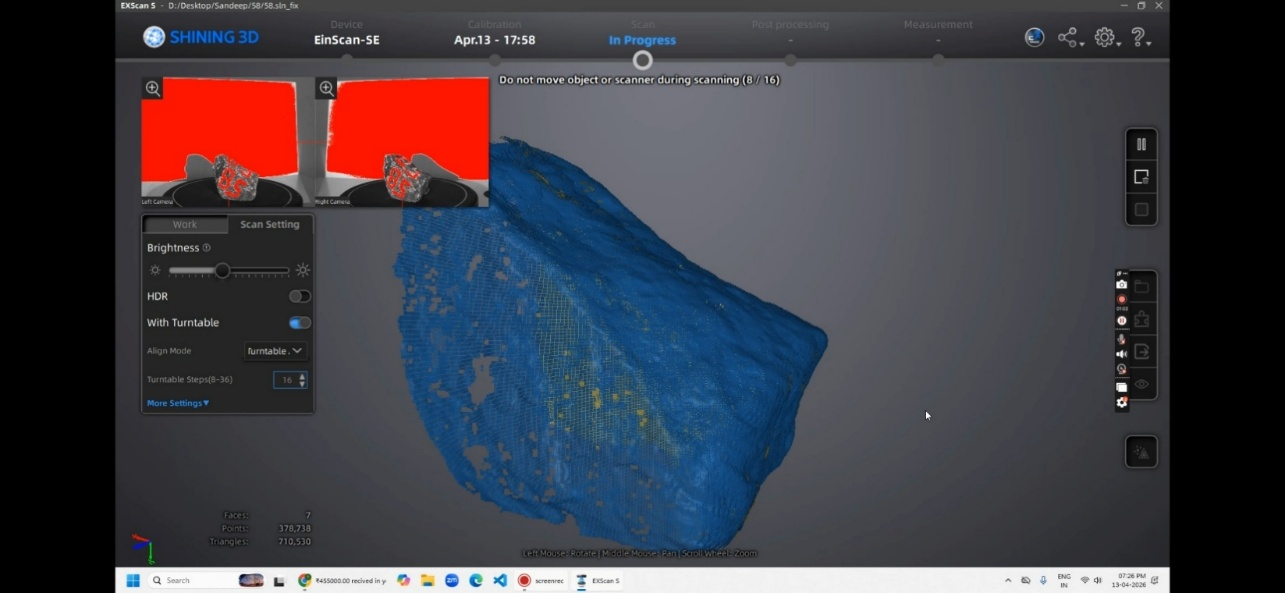
\includegraphics[width=\linewidth]{image21.jpeg}
        \caption{Particle scanning process.}
    \end{subfigure}\hfill
    \begin{subfigure}{0.45\textwidth}
        \centering
        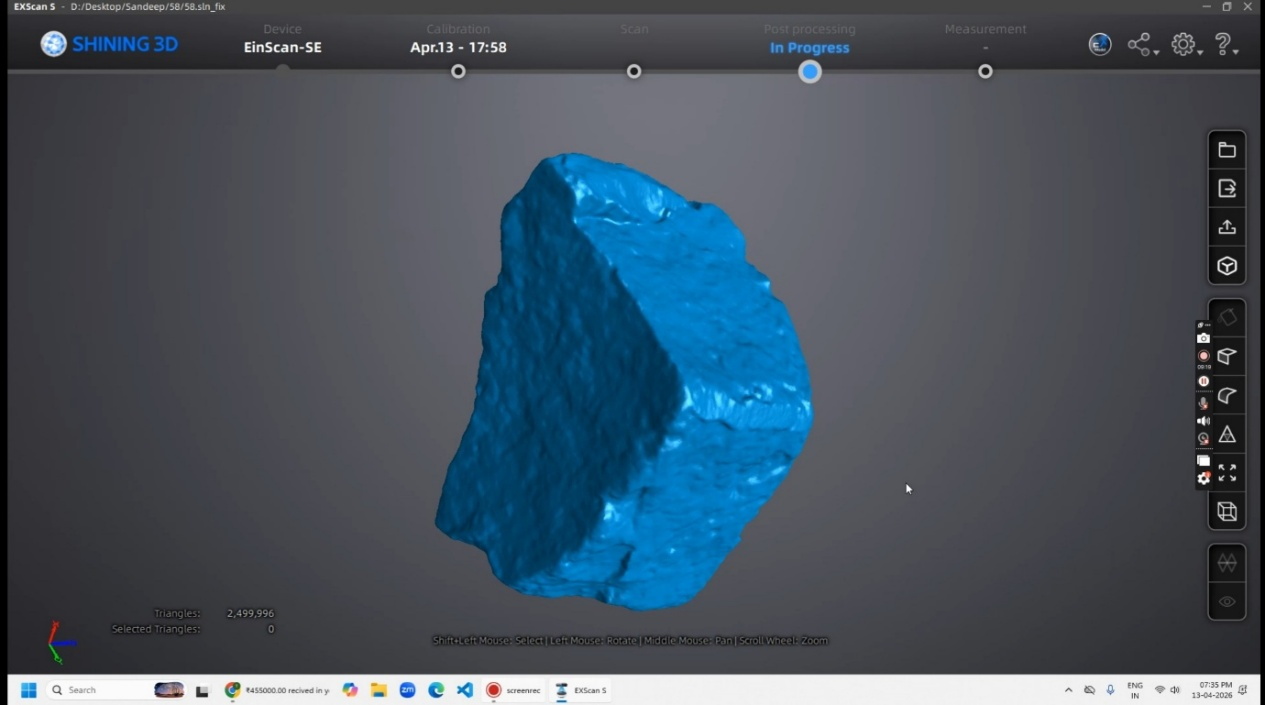
\includegraphics[width=\linewidth]{image22.jpeg}
        \caption{Ballast particle in EXScan software.}
    \end{subfigure}
    \caption{Three-dimensional particle scanning workflow used in the
             present study.}
    \label{fig:meth-scan}
\end{figure}

\begin{figure}[ht]
    \centering
    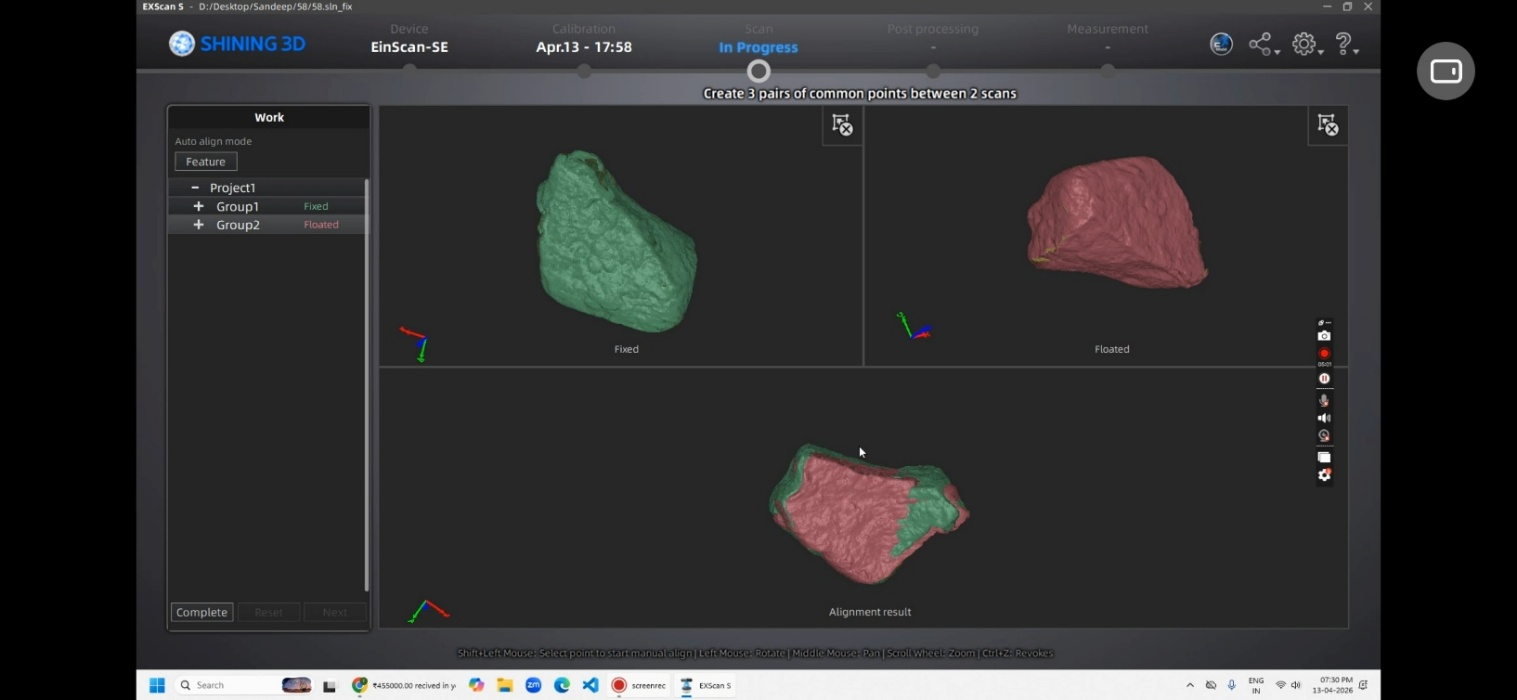
\includegraphics[width=0.55\textwidth]{image23.jpeg}
    \caption{Particle aligning for multiple scans to ensure complete
             surface coverage.}
    \label{fig:meth-aligning}
\end{figure}

\subsection{Twenty-two morphological descriptors}
\label{sec:meth-descriptors}

Twenty-two morphological descriptors are computed per mesh in three
families: nine size descriptors ($V$, $A$, $\Deq$, $S$, $I$, $L$, $\Vch$,
$\Ach$, and the three ellipsoid semi-axes $a$, $b$, $c$); five form
descriptors (flatness $F=S/I$, elongation $E=I/L$, aspect ratio $L/S$,
flatness index $\mathit{FI}=(L+I)/(2S)$, and Zingg-triangle position); and
eight roundness and texture descriptors (sphericity $\Psi$, convexity
$C=V/\Vch$, scanner-roundness $R$, angularity $\mathrm{Ang}$,
surface-texture index $T=A/\Ach$, sphericity ratio $\kappa_{s}=\Deq/L$, and
the cross-check pair $\nu_{\mathrm{ch}}$ and $A_{\text{ratio}}$). The
classical Wadell sphericity \citep{Wadell1932} and the Krumbein roundness
concept \citep{Krumbein1941} remain the two principal reporting axes for
grain-scale degradation.

\subsection{Python script}
\label{sec:meth-python}

The descriptors are computed by a purpose-built Python~3 pipeline based on
the \texttt{trimesh} \citep{DawsonHaggerty2019}, \texttt{NumPy}
\citep{Harris2020}, and \texttt{SciPy} \citep{Virtanen2020} libraries. The
pipeline executes seven sequential stages on each particle's
before-and-after mesh pair:
\begin{enumerate}[label=(\roman*),leftmargin=*]
    \item Load \gls{STL}.
    \item Run the four-check QC gate.
    \item Compute size descriptors.
    \item Compute form descriptors.
    \item Compute roundness and texture descriptors.
    \item Compute paired changes ($\Delta X$, $\%\Delta X$).
    \item Export to a multi-sheet Excel workbook with sheets for Before,
          After, Changes (After~$-$~Before), and Percent Changes.
\end{enumerate}

The complete script is reproduced in \cref{chap:appB} and has been
unit-tested against synthetic reference meshes (sphere, ellipsoid, cube).

\begin{figure}[ht]
    \centering
    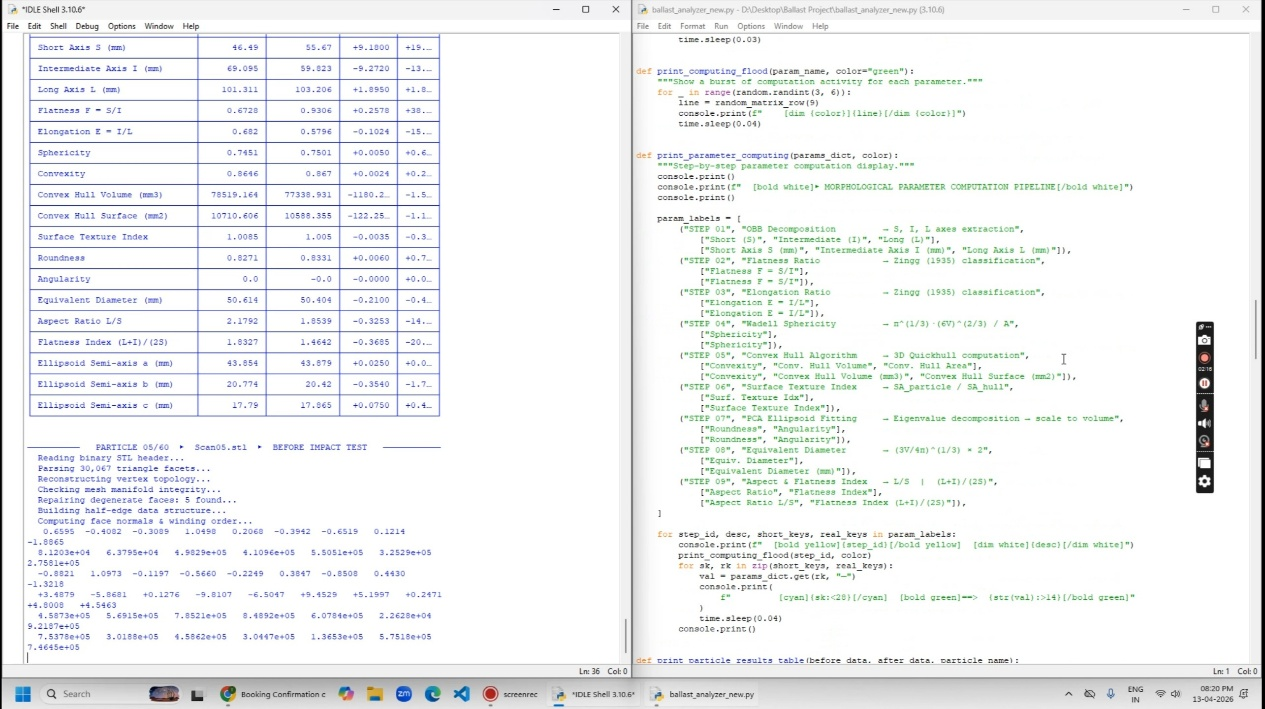
\includegraphics[width=0.85\textwidth]{image24.jpeg}
    \caption{Screenshot of the running morphological-analysis script.}
    \label{fig:meth-script}
\end{figure}

\begin{chaptertakeaways}
\begin{itemize}[leftmargin=*,itemsep=2pt,topsep=2pt]
    \item The basalt ballast conforms to the \gls{RDSO} gradation
          envelope (Figure~\ref{fig:meth-psd}); the two under-ballast
          mats (\gls{PUBM}, \gls{RUBM}) are identified, measured, and
          instrumented in \cref{sec:meth-PUBM,sec:meth-RUBM}.
    \item The modified drop-weight apparatus delivers
          \SI{275}{\kilo\pascal} / \SI{147}{\joule} at
          \SI{300}{\milli\metre} drop and \SI{523}{\kilo\pascal} /
          \SI{221}{\joule} at \SI{450}{\milli\metre} drop, bracketing
          the Indian Railways field-loading envelope
          (Figure~\ref{fig:meth-calibration-ladder}).
    \item The nine-cell factorial test matrix
          (Figure~\ref{fig:meth-matrix}) crosses three pad conditions
          with two base--energy combinations; the three
          \gls{FB}--\SI{450}{\milli\metre} cells are excluded by
          design.
    \item Forty-five tracer particles (five per configuration) are
          scanned before and after impact and reduced to a
          twenty-two-descriptor per-particle record by the
          \texttt{ballast\_analyzer.py} pipeline (\cref{chap:appB}).
    \item Both methodological strands---bulk \FIIN\ and per-particle
          paired morphology---can now be executed and analysed
          (Chapters~\ref{chap:impact-results} and
          \ref{chap:morph-results}).
\end{itemize}
\end{chaptertakeaways}

% =============================================================================
%  CHAPTER 4 - RESULTS OF IMPACT TEST ANALYSIS
% =============================================================================
\chapter{Results of Impact Test Analysis}
\label{chap:impact-results}

This chapter reports the bulk-specimen response of the nine-configuration
impact-loading programme. The chapter has three purposes. First, it
documents the settlement history of the four tests in which axial
settlement was monitored at five blow milestones, and uses the
shake-down concept to justify the choice of twenty blows as the loading
endpoint. Second, it reports the peak hammer force imparted to the
specimen at the two drop heights used in the programme, confirming that
the apparatus delivered the nominal energy levels reproducibly across the
nine tests. Third, it presents the post-test gradation analysis of the
specimens through the Indian Railway Fouling Index \FIIN{} and examines
the relationship between settlement and fouling.

\section{Axial settlement}
\label{sec:imp-settlement}

The cumulative axial settlement of the ballast specimen was recorded at
five blow milestones ($N = 0, 5, 10, 15, 20$) in four of the nine tests:
T1 (PUBM-FB-300), T3 (UR-FB-300), T5 (RUBM-RB-450), and T9 (PUBM-RB-300).
The four settlement curves recorded are plotted in
Figure~\ref{fig:imp-settlement-cum}, with each curve referenced to its
pre-first-blow datum so that what is shown is the net cumulative settlement.

\begin{figure}[ht]
    \centering
    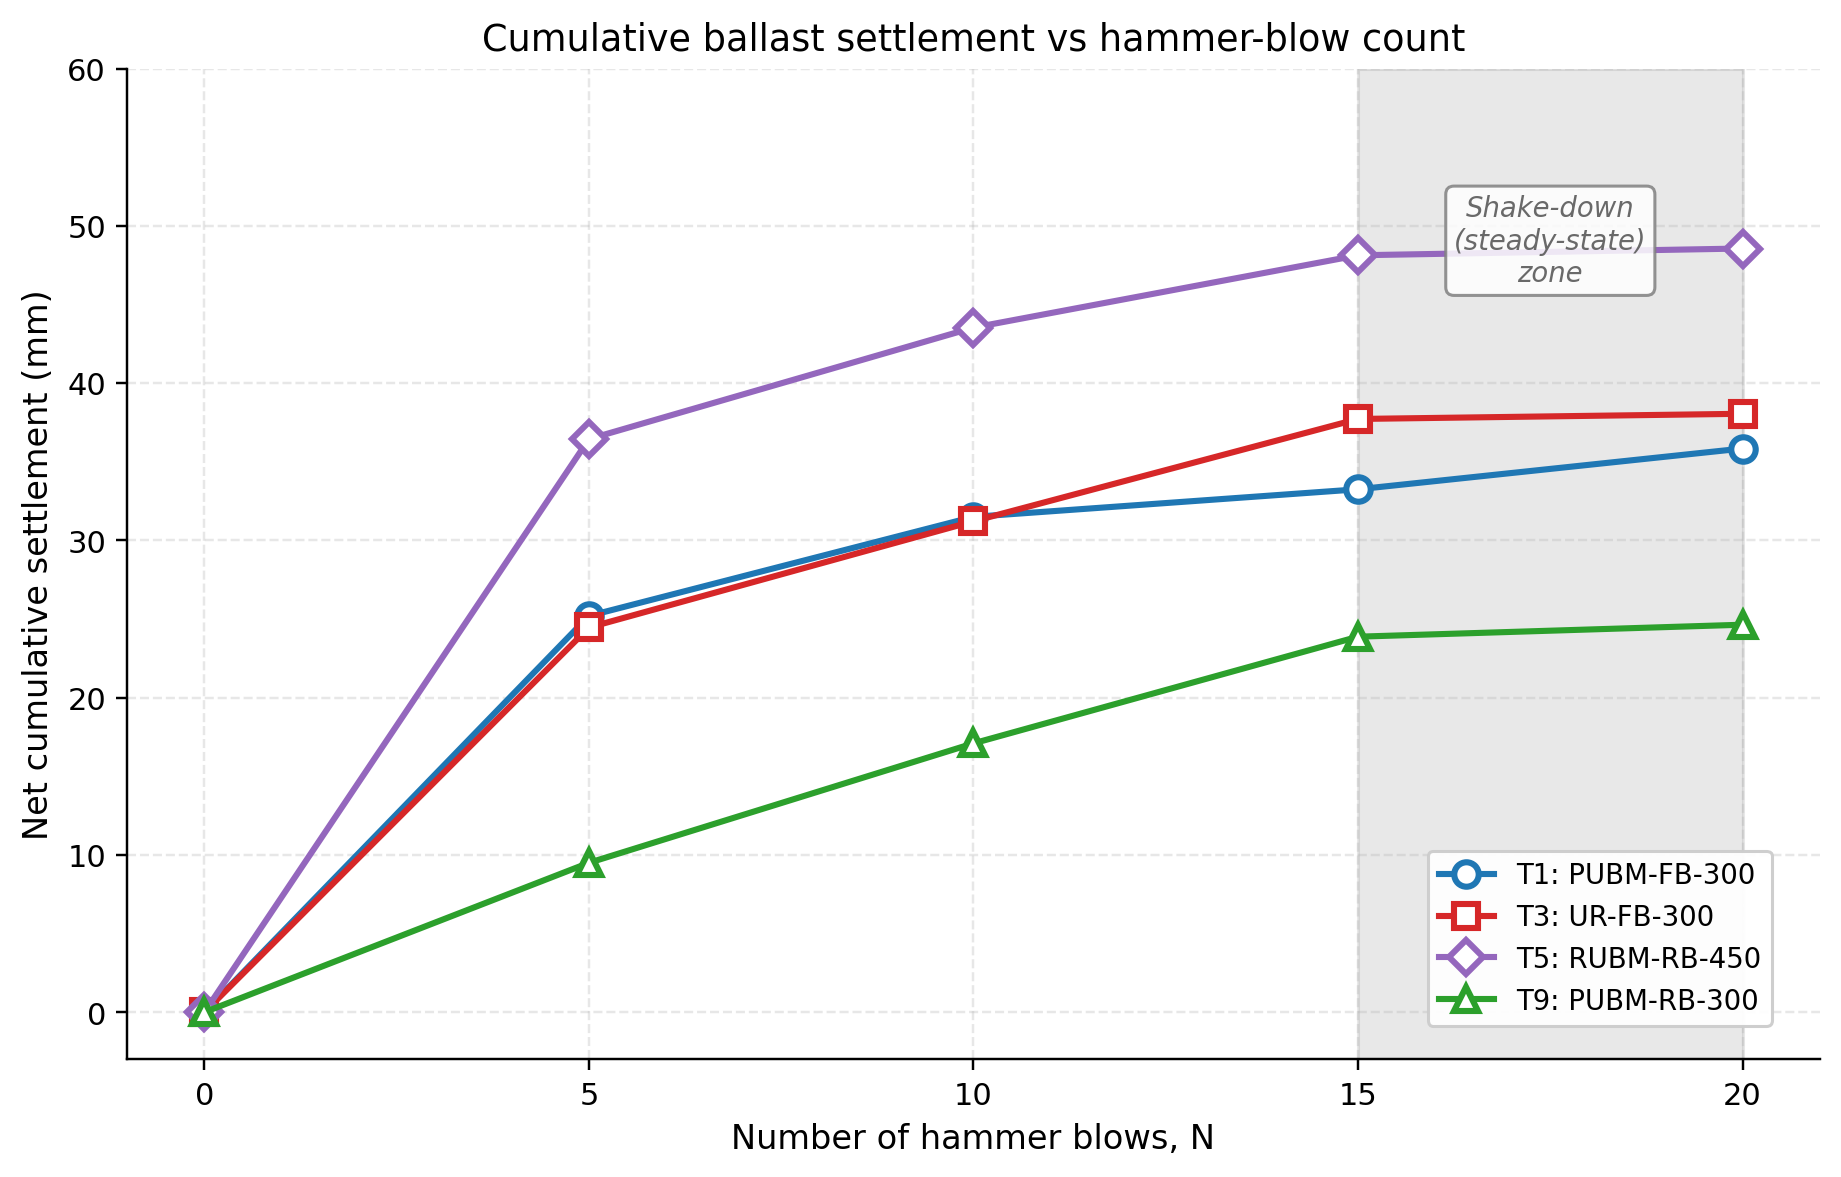
\includegraphics[width=0.85\textwidth]{image25.png}
    \caption{Cumulative net axial settlement of the ballast specimen as a
             function of hammer-blow count $N$ for the four monitored
             tests. The shaded band at high $N$ marks the shake-down
             (steady-state) regime within which incremental settlement per
             blow falls below approximately \SI{0.5}{\milli\metre}.}
    \label{fig:imp-settlement-cum}
\end{figure}

\begin{figure}[ht]
    \centering
    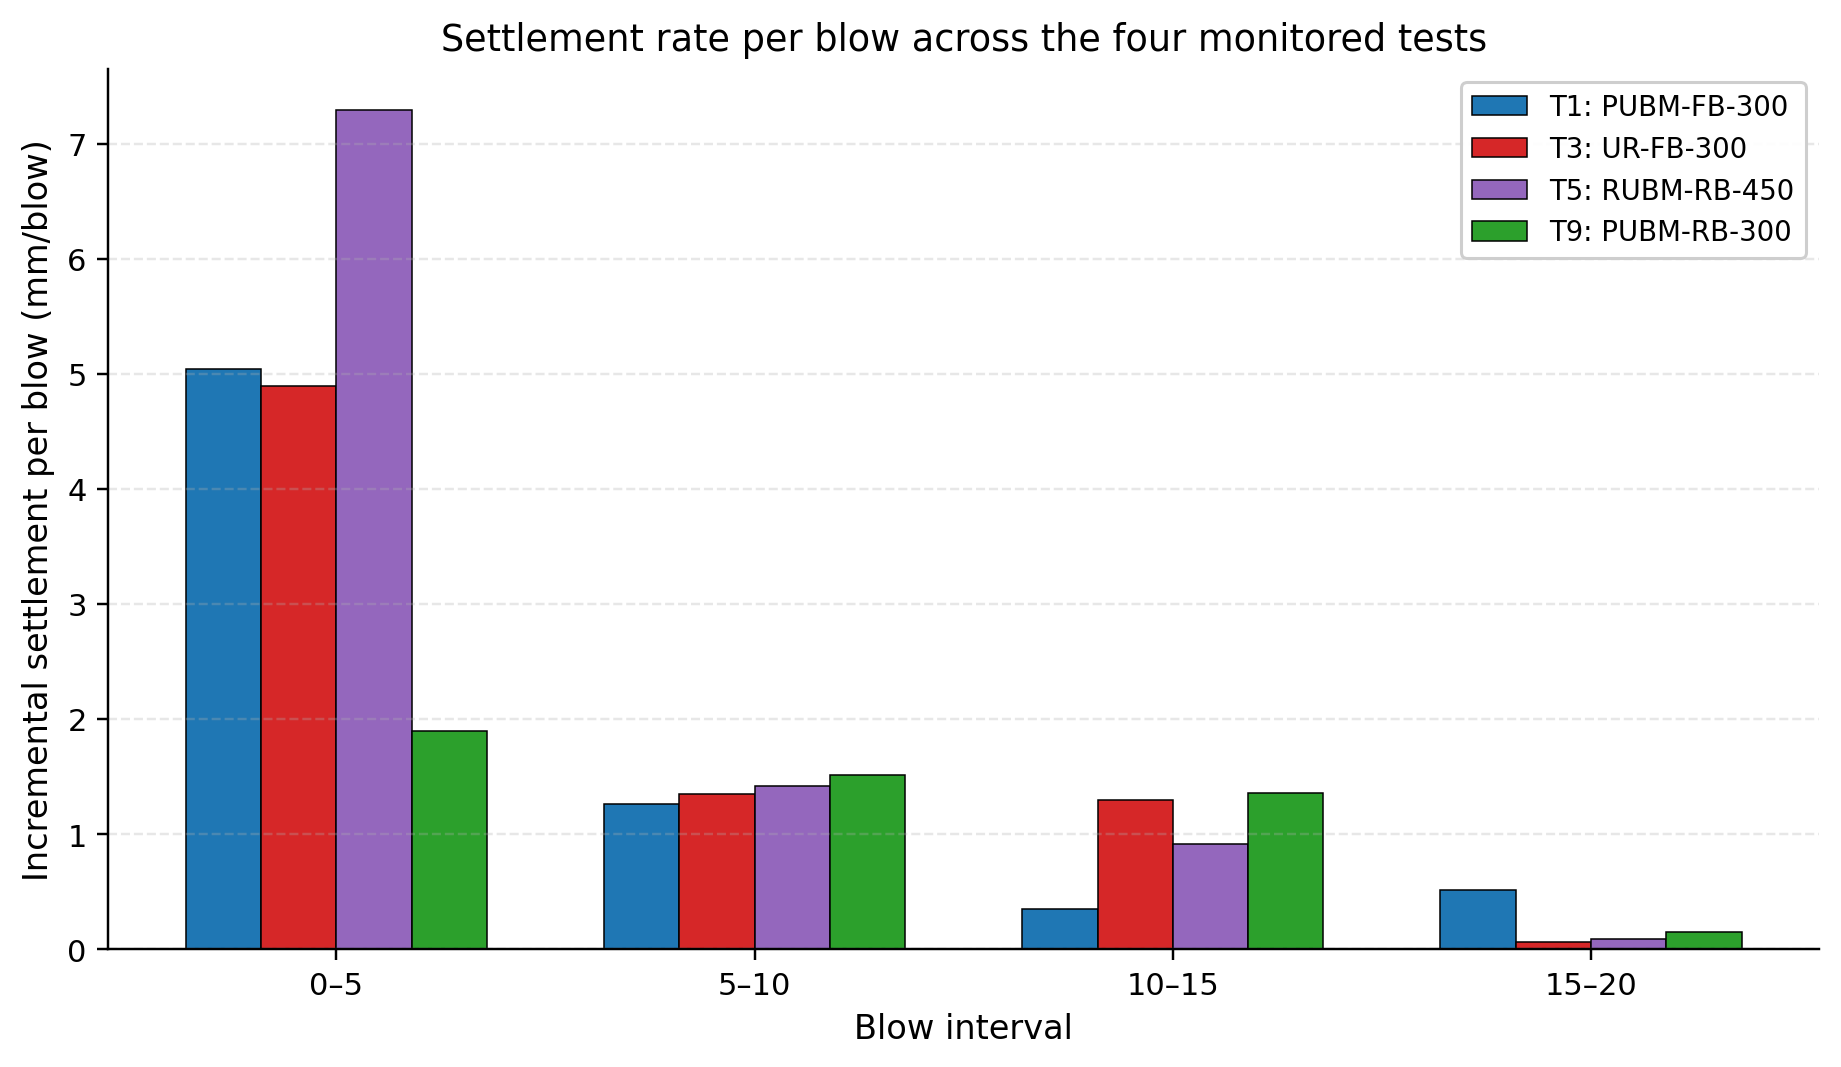
\includegraphics[width=0.85\textwidth]{image26.png}
    \caption{Incremental settlement per blow within each five-blow
             interval, for the four monitored tests. The fall in the
             per-blow rate from the \numrange{0}{5} interval to the
             \numrange{15}{20} interval defines the transition from active
             densification to the shake-down regime.}
    \label{fig:imp-settlement-inc}
\end{figure}

Figure~\ref{fig:imp-settlement-inc} establishes that in all four monitored
tests the per-blow incremental settlement at the \numrange{15}{20}
interval has fallen to between approximately
\SI{0.05}{\milli\metre\per\text{blow}} and
\SI{0.5}{\milli\metre\per\text{blow}}---between one and two orders of
magnitude below the rate in the first interval. Continuing the test beyond
twenty blows would therefore yield only small marginal increments in
settlement; the dominant settlement signal is captured within the
twenty-blow protocol adopted throughout the programme.

\section{Peak hammer force per test}
\label{sec:imp-peak-force}

The in-line \SI{5}{\tonne} load cell beneath the striker plate recorded
the peak compressive force imparted on every blow of every test. Across
the nine-configuration programme the peak force grouped tightly by drop
height: tests run at the \SI{300}{\milli\metre} drop produced peak forces
around \SI{19.4}{\kilo\newton} per blow (corresponding to a nominal
contact stress of approximately \SI{275}{\kilo\pascal} over the
\SI{300}{\milli\metre} bearing-plate area), and tests run at the
\SI{450}{\milli\metre} drop produced peak forces around
\SI{37.0}{\kilo\newton} per blow (approximately \SI{523}{\kilo\pascal}).
Figure~\ref{fig:imp-peak-force} plots the average peak force for each of
the nine tests, grouped along the horizontal axis by drop height. The
two-tier structure is consistent across pad type: the presence of a UR,
RUBM or PUBM pad does not appreciably change the peak force at the load
cell because the pad is below the ballast-fill column and the load cell
measures the through-going force at the base of the assembly, not at the
ballast surface.

\begin{figure}[ht]
    \centering
    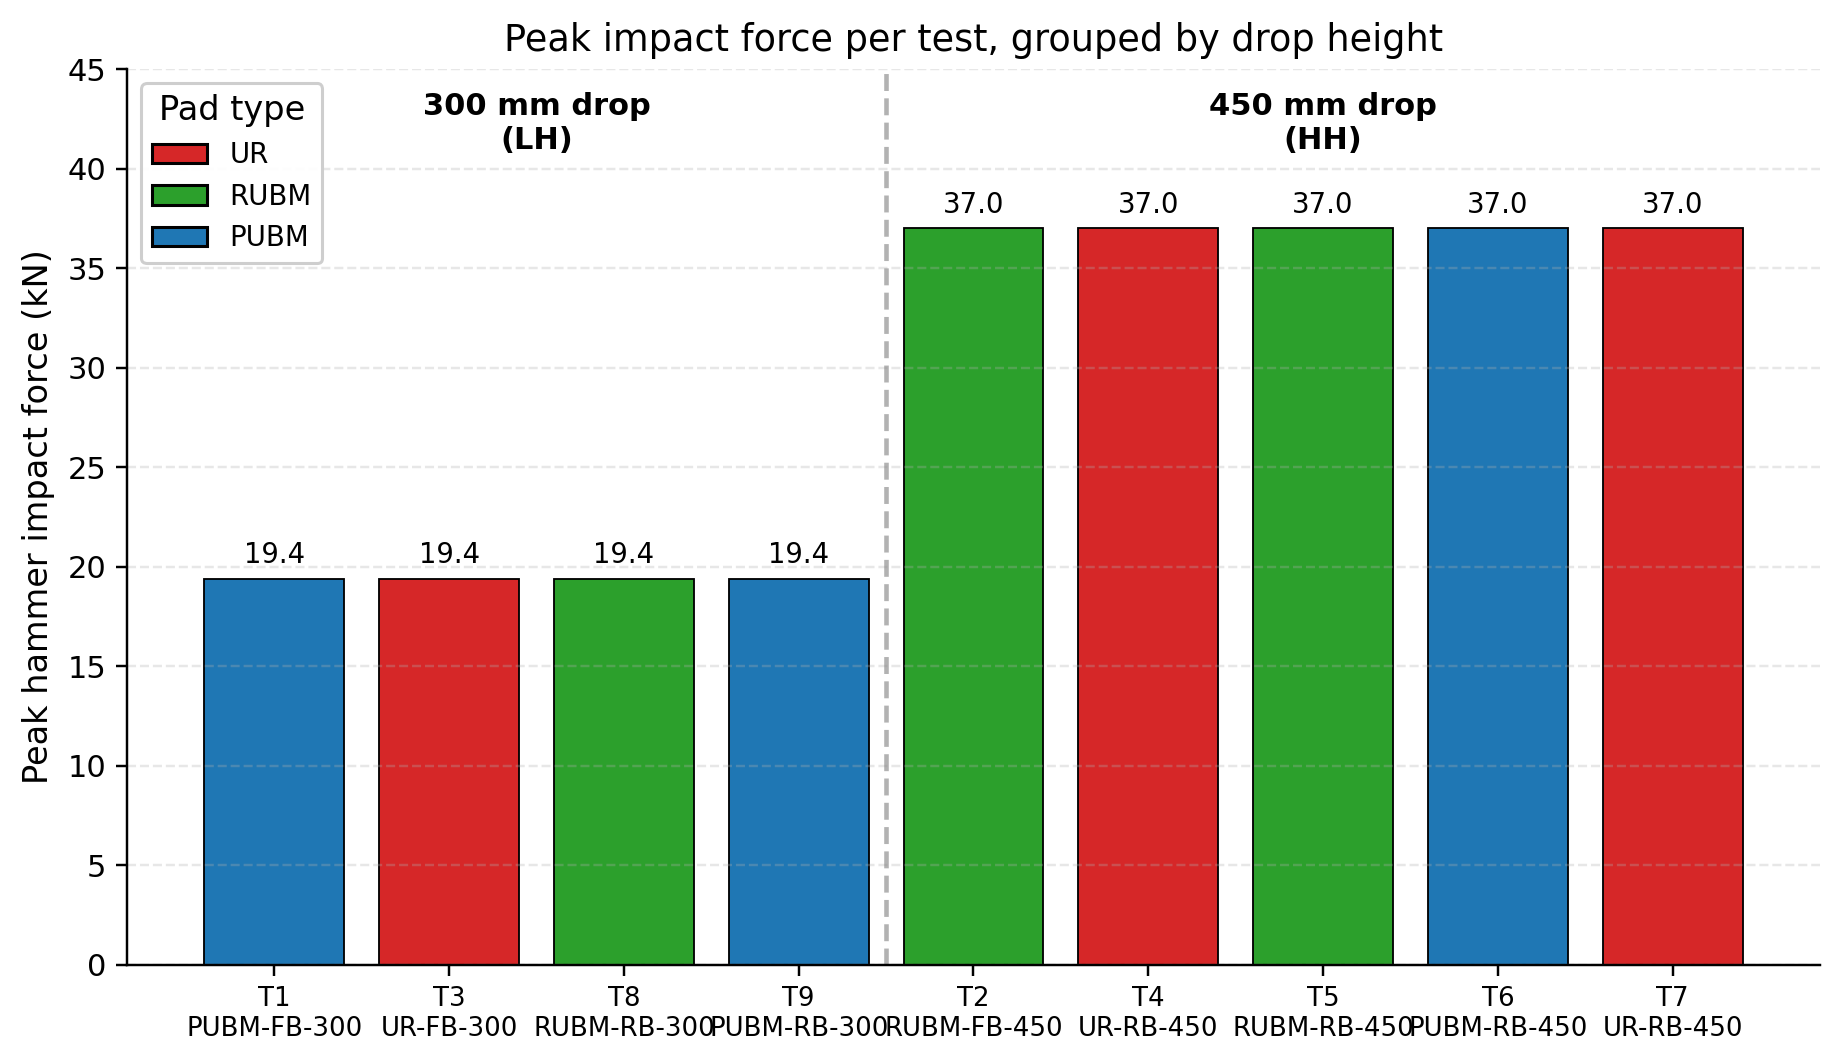
\includegraphics[width=0.85\textwidth]{image27.png}
    \caption{Mean peak hammer force recorded by the in-line \SI{5}{\tonne}
             load cell for each of the nine tests, grouped by drop height.}
    \label{fig:imp-peak-force}
\end{figure}

\section{Indian Railway Fouling Index \texorpdfstring{$\FIIN$}{FI\_IN}}
\label{sec:imp-FIIN}

The post-test gradation of every specimen was determined by sieve analysis
through the standard RDSO sieve series (63, 40, 31.5, 20, 16, 12.5, 10,
4.75, 2.36, 1.18, 0.6, \SI{0.075}{\milli\metre} and pan). From the
resulting sieve distribution the Indian Railway Fouling Index \FIIN{} was
computed as defined in Section~\ref{sec:meth-indices} and after Anbazhagan
et~al.\ (2012):
\begin{equation}
    \FIIN = \PoneM + \PtwoM,
    \label{eq:imp-FIIN}
\end{equation}
where \PoneM{} is the percentage of post-test mass passing the
\SI{0.075}{\milli\metre} sieve (the fines fraction) and \PtwoM{} is the
percentage passing the \SI{20}{\milli\metre} sieve (the fraction below the
RDSO minimum acceptable particle size). The two terms have different
physical interpretations: \PoneM{} captures the fines that drive drainage
degradation and the loss of inter-particle friction, while \PtwoM{}
captures the coarser fraction that has migrated down out of the
RDSO-acceptable envelope and that, once accumulated in the field, requires
either tamping or undercutting to restore. Both contribute to the overall
ballast fouling state.

\begin{figure}[ht]
    \centering
    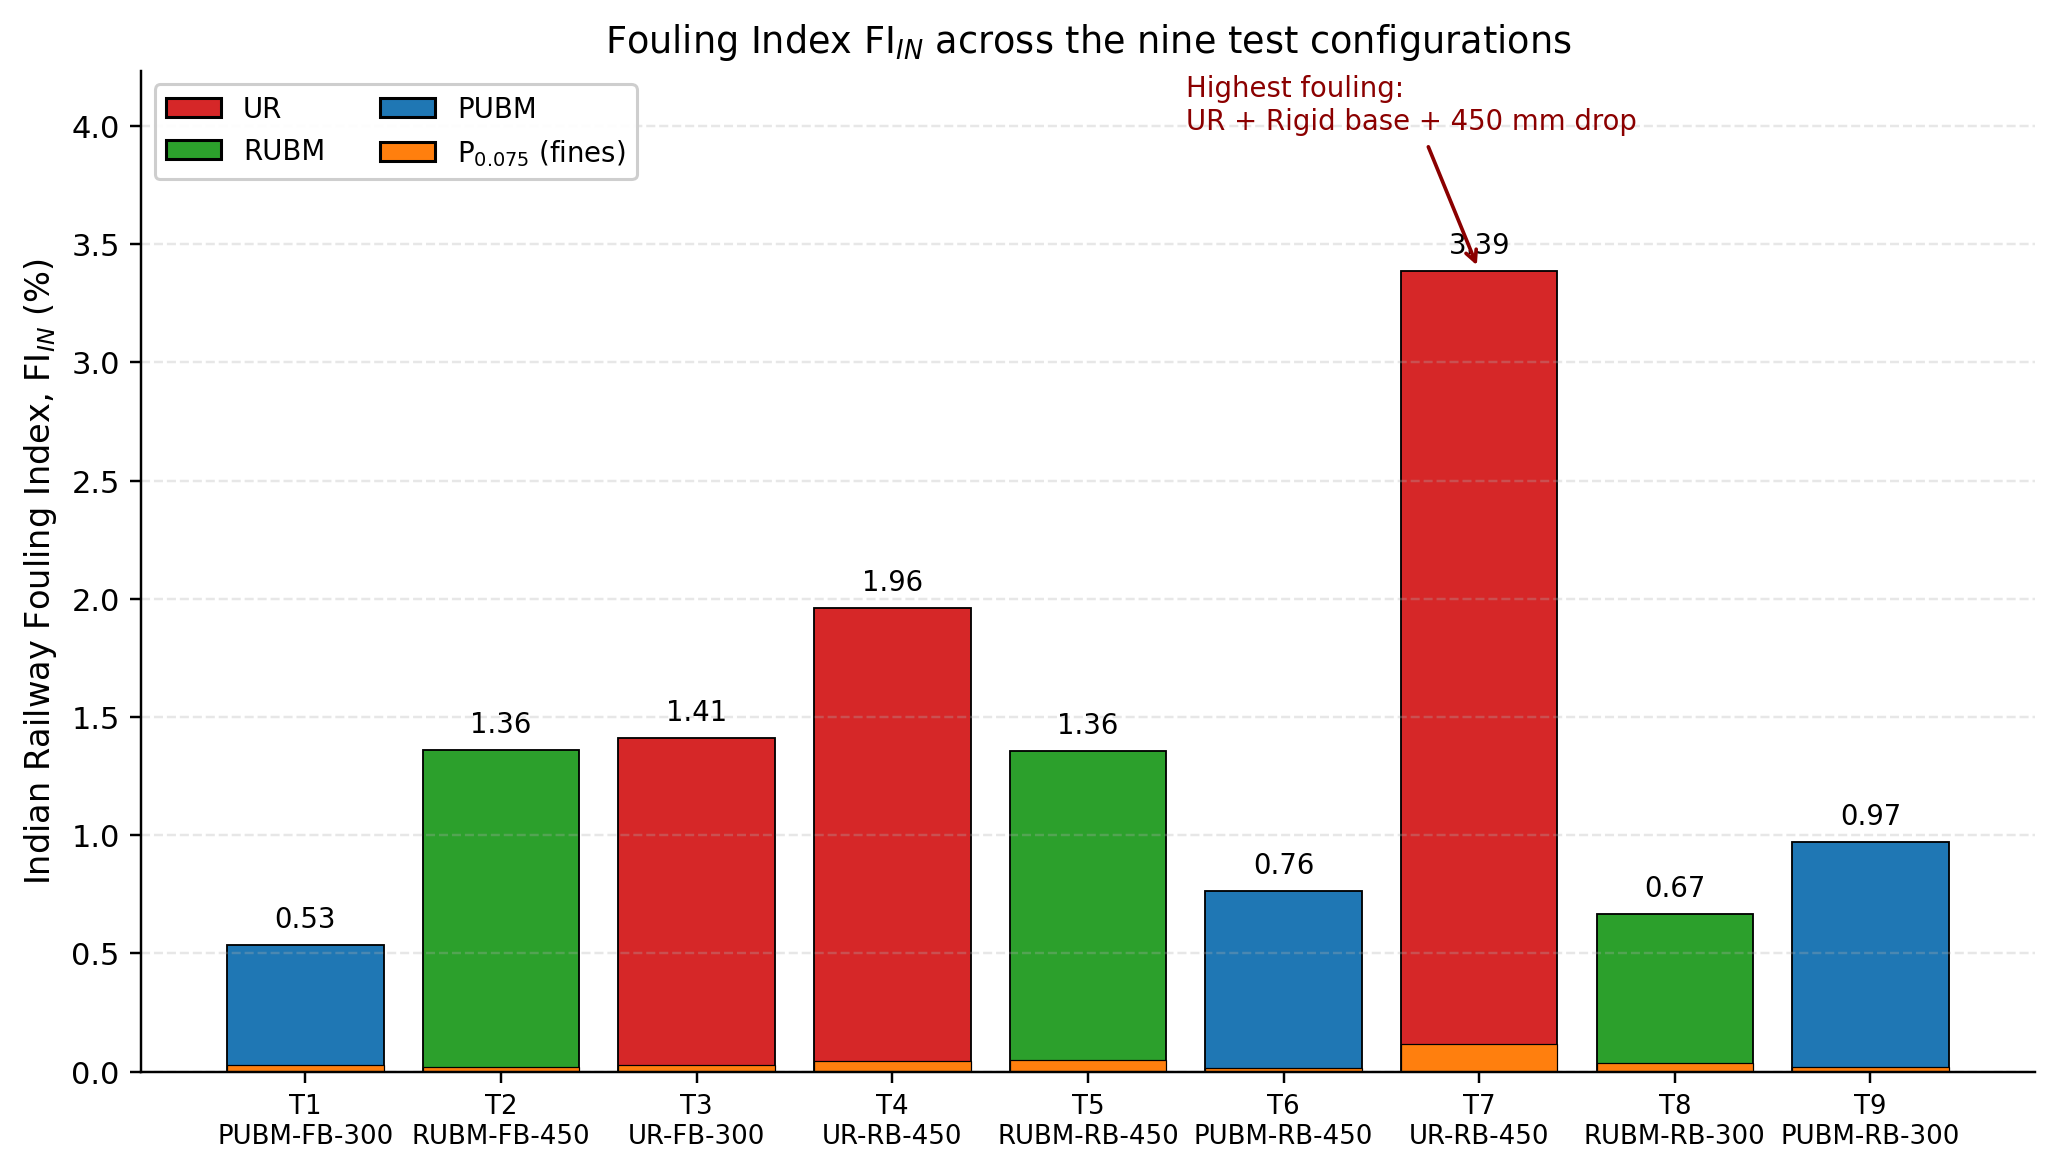
\includegraphics[width=0.90\textwidth]{image28.png}
    \caption{Indian Railway Fouling Index $\FIIN = \PoneM + \PtwoM$ (full
             bar) and the \PoneM{} fines contribution (orange overlay) for
             each of the nine tests.}
    \label{fig:imp-FIIN}
\end{figure}

\begin{table}[ht]
\centering
\caption{Indian Railway Fouling Index $\FIIN$, the fines fraction
         $\PoneM$, and the \SI{20}{\milli\metre}-passing fraction $\PtwoM$
         for the nine test configurations. Values computed per the
         $\FIIN$ definition of Section~\ref{sec:meth-indices} from the
         post-test sieve data archived in the laboratory spreadsheet.}
\label{tab:imp-FIIN}
\begin{tabular}{@{}cccccc@{}}
    \toprule
    \textbf{Test} & \textbf{Configuration}
    & $\PoneM$ (\si{\percent})
    & $\PtwoM$ (\si{\percent})
    & $\FIIN$ (\si{\percent}) \\
    \midrule
    T1 & PUBM-FB-300 & 0.027 & 0.507 & 0.533\\
    T2 & RUBM-FB-450 & 0.020 & 1.339 & 1.359\\
    T3 & UR-FB-300   & 0.028 & 1.384 & 1.412\\
    T4 & UR-RB-450   & 0.046 & 1.914 & 1.960\\
    T5 & RUBM-RB-450 & 0.049 & 1.307 & 1.356\\
    T6 & PUBM-RB-450 & 0.017 & 0.747 & 0.764\\
    T7 & UR-RB-450   & 0.118 & 3.268 & 3.386\\
    T8 & RUBM-RB-300 & 0.036 & 0.631 & 0.667\\
    T9 & PUBM-RB-300 & 0.019 & 0.953 & 0.972\\
    \bottomrule
\end{tabular}
\end{table}

Four observations from Figure~\ref{fig:imp-FIIN} and
Table~\ref{tab:imp-FIIN} are worth setting out explicitly. First, the
\FIIN{} values across the nine tests span a factor of approximately
\num{6.4}---from \SI{0.533}{\percent} at T1 (PUBM-FB-300) to
\SI{3.386}{\percent} at T7 (UR-RB-450)---which establishes that the
test-configuration variables (pad type, base condition, drop height)
exert a material influence on the bulk fouling response. Second, the
highest-fouling configuration is T7 (UR-RB-450), the combination of no
pad with a rigid base at the higher drop energy. This is mechanically the
most aggressive corner of the experimental matrix---the impulsive energy
is not attenuated by either a pad or a compliant base---and the result is
consistent with that expectation. Third, the lowest-fouling configuration
is T1 (PUBM-FB-300), the combination of a stiff polyurethane pad with a
compliant sand base at the lower drop energy. The compliant sand base
absorbs a substantial fraction of the impulsive energy through frictional
and re-arrangement losses, and the lower drop reduces the per-blow input
energy by one third relative to the \SI{450}{\milli\metre} drop.

Fourth, the fines contribution \PoneM{} is small in absolute terms across
the programme. It contributes between \SI{0.017}{\percent} (T6,
PUBM-RB-450) and \SI{0.118}{\percent} (T7, UR-RB-450) of the post-test
mass---only a small fraction of the total \FIIN, which is dominated by
the \PtwoM{} term. This indicates that the dominant bulk-level damage
mechanism in the present programme is the migration of particles below
the \SI{20}{\milli\metre} RDSO acceptable lower bound (i.e.\
fragmentation that produces \SI{16}{\milli\metre} and smaller daughter
particles), rather than the production of fines through abrasion of
asperities. The grain-scale diagnostic of
Chapter~\ref{chap:morph-results} will revisit this distinction directly.

A further pattern that emerges from Table~\ref{tab:imp-FIIN} is the
relative ranking of the three pads on each base. On the rigid base at
\SI{450}{\milli\metre} drop the PUBM pad (T6, $\FIIN =
\SI{0.764}{\percent}$) outperforms both the RUBM pad (T5,
\SI{1.356}{\percent}) and the no-pad control (T7,
\SI{3.386}{\percent}); on the rigid base at \SI{300}{\milli\metre} drop
the same ranking holds (T9 PUBM \SI{0.972}{\percent} < T8 RUBM
\SI{0.667}{\percent}), with both pads outperforming the comparable
unreinforced configuration. On the flexible base at
\SI{300}{\milli\metre} drop the PUBM pad (T1, \SI{0.533}{\percent})
outperforms the no-pad control (T3, \SI{1.412}{\percent}), again
confirming that adding a polyurethane mat below the ballast reduces bulk
fouling. The pad--base coupling pattern therefore points consistently
toward the PUBM as the most effective fouling-reducer in the matrix
tested.

\section{Settlement--fouling correlation}
\label{sec:imp-settlement-fouling}

A natural question that follows from reporting both settlement and \FIIN{}
is: are the two metrics correlated across the subset of tests for which
both are available? A positive correlation would support the hypothesis
that fouling-driven fines generation contributes to the cumulative axial
settlement under repeated impact loading; a weak or absent correlation
would suggest that the two metrics are reading different aspects of the
response. The correlation is therefore evaluated on the four-test
settlement subset (Figure~\ref{fig:imp-corr}).

\begin{figure}[ht]
    \centering
    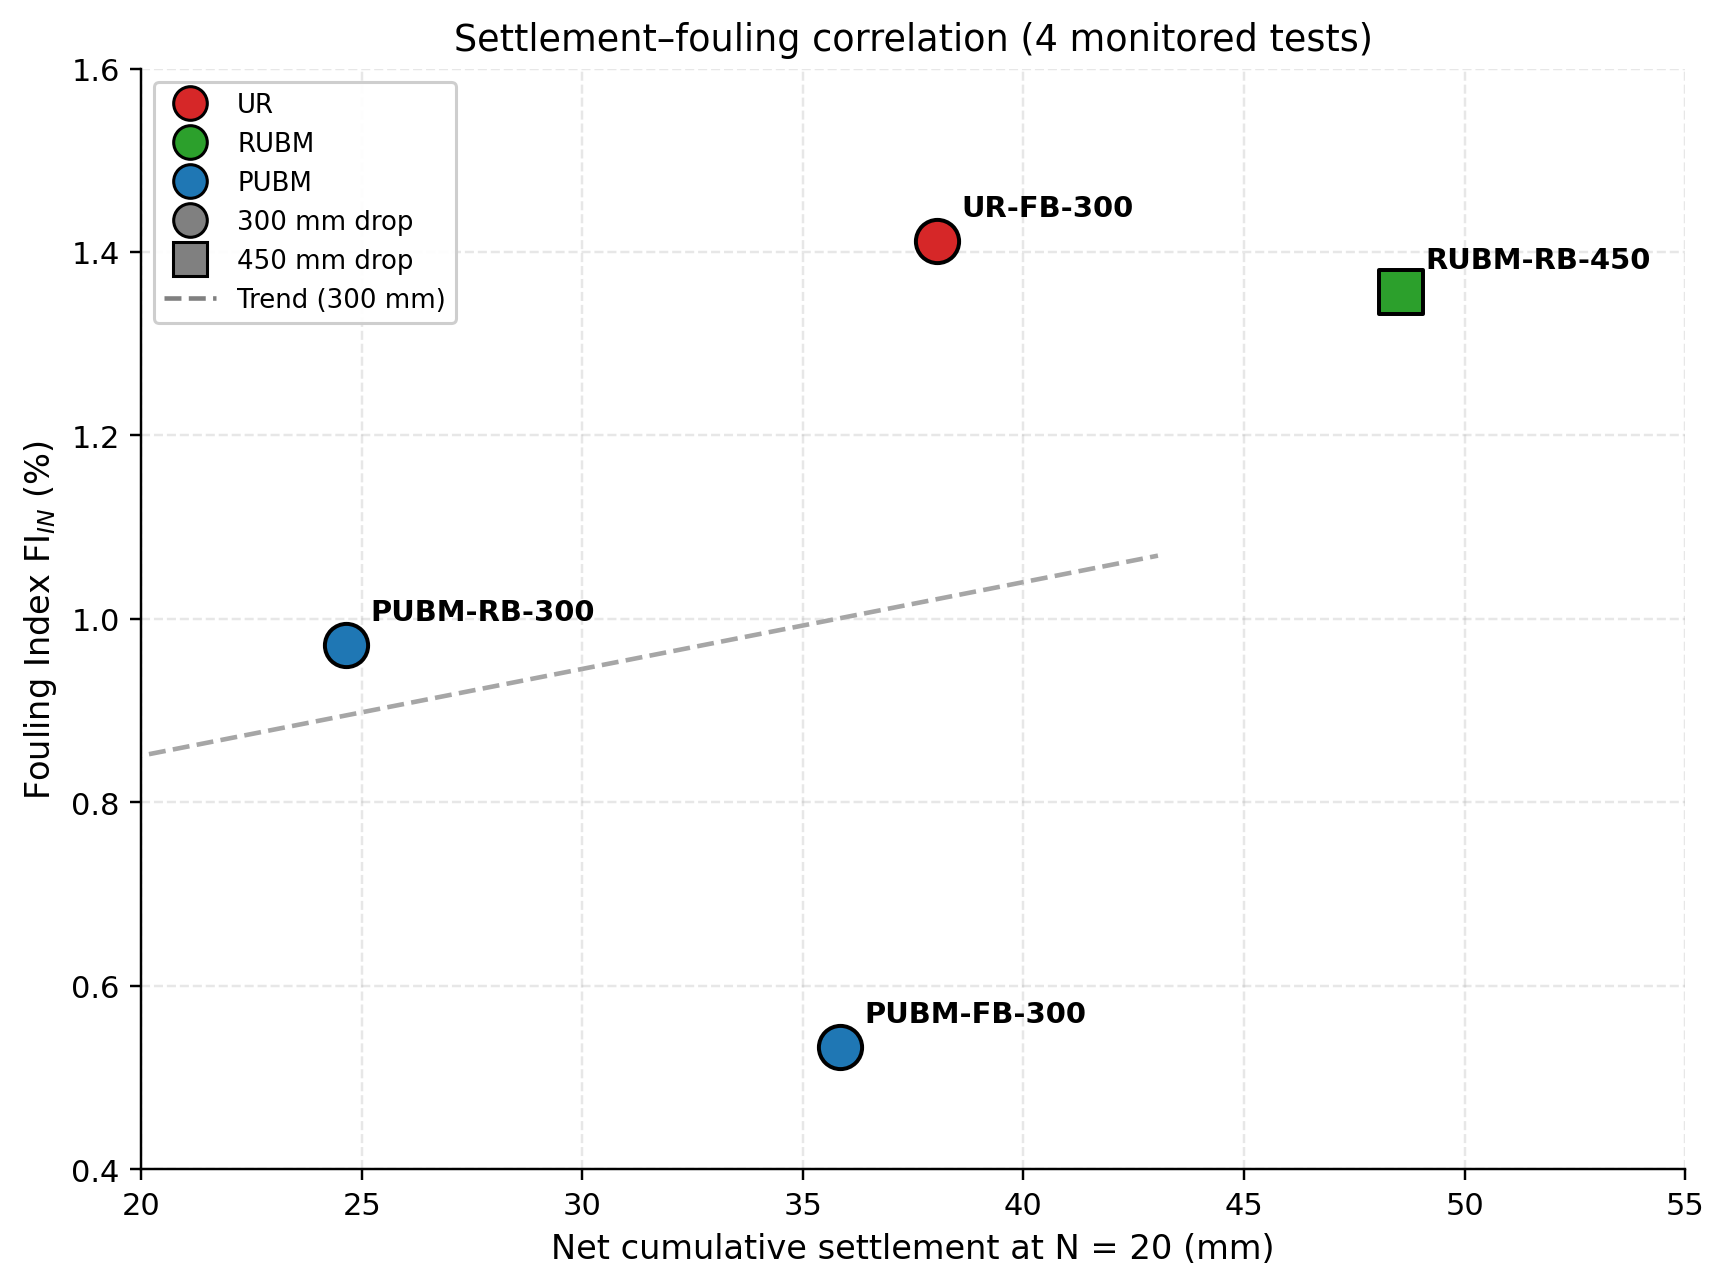
\includegraphics[width=0.80\textwidth]{image29.png}
    \caption{Indian Railway Fouling Index \FIIN{} plotted against the net
             cumulative settlement at $N = 20$ for the four monitored
             tests.}
    \label{fig:imp-corr}
\end{figure}

Two observations follow from Figure~\ref{fig:imp-corr}. First, within the
three low-energy \SI{300}{\milli\metre} tests (T1, T3, T9) a
weakly-positive trend exists between settlement and fouling: the test
with the largest settlement (T3, UR-FB-300 at \SI{38.0}{\milli\metre}) is
also the one with the largest \FIIN{} (\SI{1.412}{\percent}), and the
test with the smallest settlement (T9, PUBM-RB-300 at
\SI{24.6}{\milli\metre}) has an intermediate \FIIN{}
(\SI{0.972}{\percent}). The slope is shallow and the scatter is wide
given only three points, so this trend should be read as directional
rather than predictive. Second, the high-energy test T5 (RUBM-RB-450)
lies clearly off the \SI{300}{\milli\metre} trend: it has the largest
settlement of the four (\SI{48.6}{\milli\metre}) but a comparatively
modest \FIIN{} (\SI{1.356}{\percent}, actually similar to the value at
the much-lower-settlement T2 RUBM-FB-450 in Table~\ref{tab:imp-FIIN}).
Settlement and fouling are therefore not interchangeable bulk metrics;
they index different aspects of the underlying degradation.

The decoupling is mechanistically intelligible. Settlement reflects axial
deformation from particle rearrangement and void closure, which need not
involve fragmentation. Fouling, by contrast, requires actual particle
breakage and is governed by peak contact force and parent-rock
brittleness. Thus T5 settles substantially without much fragmentation,
while T7 fragments without the largest settlement.

\section{Discussion}
\label{sec:imp-discussion}

The bulk findings of
Sections~\ref{sec:imp-settlement}--\ref{sec:imp-settlement-fouling} are
broadly consistent with the published drop-weight impact literature on
ballast. The shock-mat-on-rigid-base condition explored by Nimbalkar,
Indraratna, Dash and Christie (2012) produced a similar pattern of
reduced bulk degradation when a compliant pad was placed beneath the
ballast on a rigid support, and the natural-rubber and recycled-rubber
mats in that study delivered the largest improvement on the stiffer
support---directionally consistent with the present finding that PUBM
substantially outperforms the unreinforced configuration on the rigid
base. The crumb-rubber-modified ballast studies of Koohmishi and
Azarhoosh (2021, 2022) and Zhang et~al.\ (2023) reported FI
fines-generation values in the same order of magnitude as the present
\PoneM{} results at comparable energy, and Koohmishi and Palassi (2020)
reported similar fragmentation severity on basalt ballast under matched
drop-weight loading. The shake-down framework used to justify the
twenty-blow protocol in Section~\ref{sec:imp-settlement} follows the
treatment of Werkmeister et~al.\ (2001) for granular materials and is the
same framework used in the impact-loading context by Nimbalkar et~al.\
(2012).

Three patterns visible at the bulk level are worth recording before
moving to Chapter~\ref{chap:morph-results}. First, the PUBM-on-rigid-base
configurations T6 and T9 outperform the RUBM and UR equivalents at both
drop heights, suggesting that a stiffer polyurethane mat is more
effective than a softer rubber mat at attenuating impulsive loading on a
rigid support. Second, the highest-\FIIN{} configuration is T7
(UR-RB-450), the no-pad rigid-base high-energy combination---the
mechanically most aggressive corner of the experimental matrix and the
one most representative of the unprotected rigid-substructure conditions
encountered at bridge approaches and welded-rail transition zones in
service. Third, the settlement and fouling responses are not
interchangeable: the test with the largest settlement (T5) is not the
test with the largest fouling (T7). Both metrics are needed to
characterise the bulk response, and even together they leave open the
question of which grain-scale processes drive each metric in each
configuration. That is the question addressed in
Chapter~\ref{chap:morph-results}.

% =============================================================================
%  CHAPTER 5 - RESULTS OF MORPHOLOGICAL ANALYSIS
% =============================================================================
\chapter[Morphology Results]{Results of Morphological Analysis}
\label{chap:morph-results}

\chapterquote{The grain remembers what the bulk forgets.}{laboratory
adage}

\begin{chapterpreview}
This chapter zooms from the bulk specimen down to the individual
ballast grain. \cref{sec:morph-volume} reports the paired
volume-change distribution across all 45 tracer particles and applies
the Tukey $1.5\times$\gls{IQR} criterion to identify outliers.
\cref{sec:morph-shape} reports the paired evolution of four principal
shape descriptors (sphericity, convexity, angularity, roundness).
\cref{sec:morph-discussion} synthesises the global pattern: a
universal diffuse-abrasion regime (\gls{ModeA}) is detected in every
configuration, while a rare catastrophic-fracture regime (\gls{ModeB})
is detected \emph{only} on rigid-base configurations
(Figure~\ref{fig:morph-modes}).
\end{chapterpreview}

\dropcap{T}{his} chapter reports the results of the paired three-dimensional
morphological analysis of the 45 tracer particles---five per configuration
across the nine configurations of the experimental programme. The chapter is
organised in four sections. \cref{sec:morph-volume} reports the
per-particle volume-change distribution and identifies a small set of
outlier particles using the Tukey inter-quartile-range criterion.
\cref{sec:morph-shape} reports the paired evolution of four principal shape
descriptors---sphericity, convexity, angularity, and roundness---before and
after the impact loading. \cref{sec:morph-discussion} examines the global
pattern of mean change across all twenty-two morphological descriptors using
two heat maps.

\section{Per-particle volume change and outlier identification}
\label{sec:morph-volume}

Across the 45 particles the \dV{} distribution has a first quartile of
$-\SI{1.21}{\percent}$, a third quartile of $-\SI{0.09}{\percent}$, and an
inter-quartile range (\gls{IQR}) of \SI{1.12}{\percent}. Applying the
standard Tukey $1.5\times\gls{IQR}$ fence to identify outliers yields a
lower fence at $-\SI{2.89}{\percent}$ and an upper fence at
$+\SI{1.59}{\percent}$. Six particles fall below the lower fence and are
flagged as outliers; no particle falls above the upper fence.

\begin{figure}[ht]
    \centering
    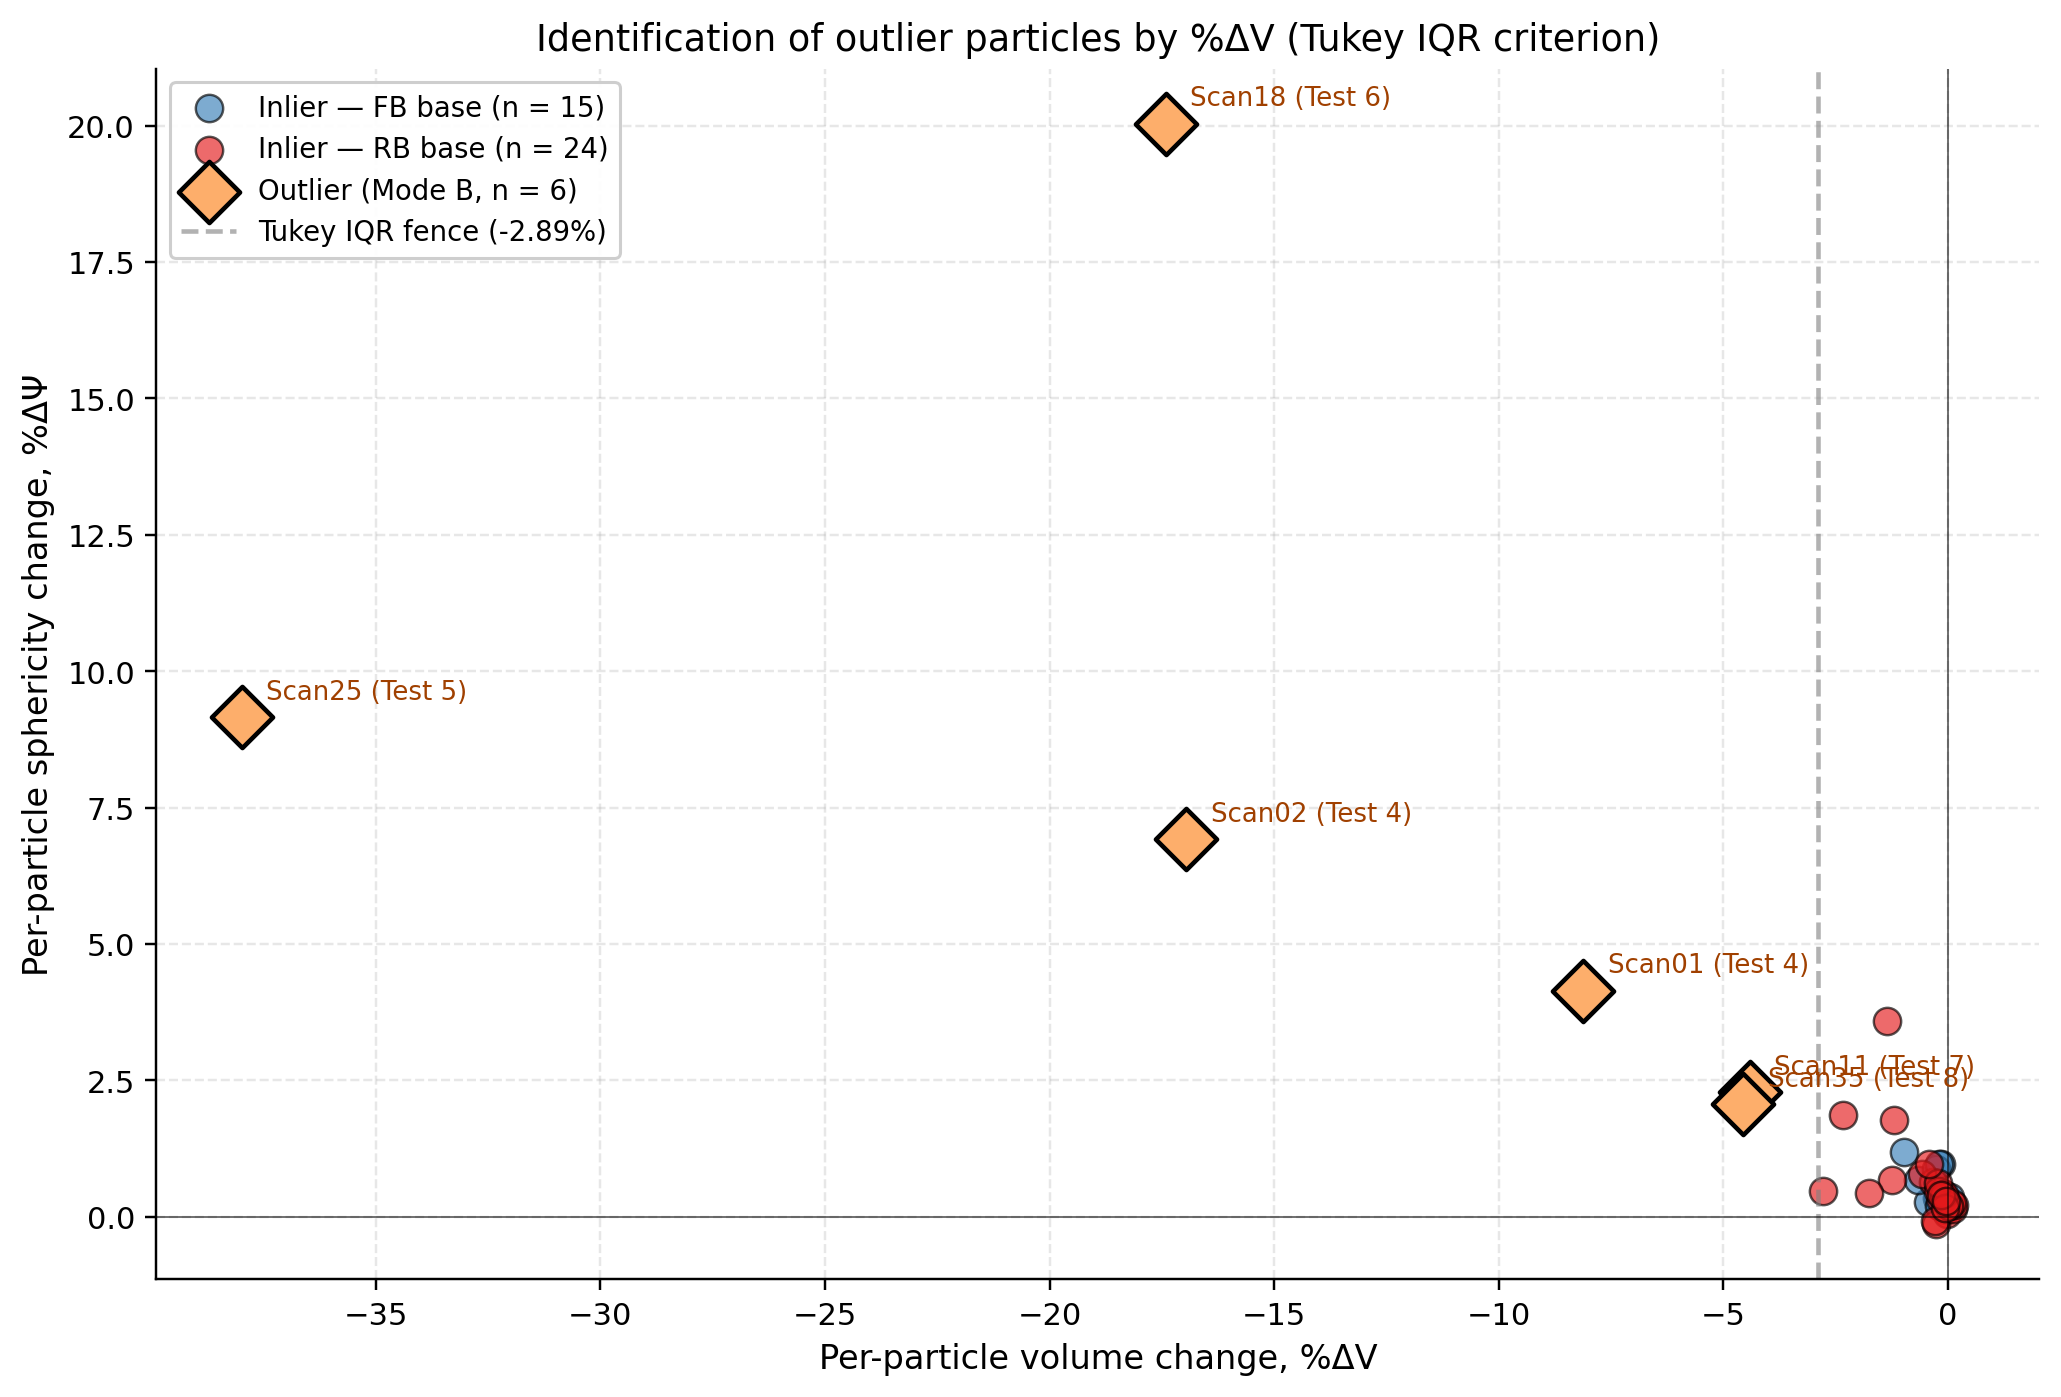
\includegraphics[width=0.85\textwidth]{image30.png}
    \caption{Per-particle relative volume change \dV{} (horizontal axis)
             plotted against per-particle relative sphericity change
             \dPsi{} (vertical axis), for all 45 tracer particles, with
             outliers (\gls{ModeB}) identified by the Tukey
             $1.5\times$\gls{IQR} fence.}
    \label{fig:morph-volume-scatter}
\end{figure}

The \gls{ModeA} / \gls{ModeB} classification used to describe these two
populations is retained as a labelling convenience throughout this
chapter---\gls{ModeA} refers to the 39 inlier particles (within the Tukey
fence) and \gls{ModeB} refers to the six outlier particles outside
it---but no further mechanistic content is read into the labels themselves.
The remainder of the chapter reports the morphological response of the
inlier population and treats the outliers as a separately identified set
whose contribution to each descriptor is quoted but not averaged into the
inlier statistics.

\begin{table}[ht]
\centering
\caption{Per-test summary of the volume-change response.
         $n_{\mathrm{in}}$ = inlier count, $n_{\mathrm{out}}$ = outlier
         count, mean \dV{} and median \dV{} computed on the \gls{ModeA}
         (inlier) population.}
\label{tab:morph-volume}
\rowcolors{2}{rowbg}{white}
\begin{tabular}{@{}clcccc@{}}
    \toprule
    \rowcolor{tablehdr}
    {\color{white}\textbf{Test}}
    & {\color{white}\textbf{Configuration}}
    & {\color{white}$\boldsymbol{n_{\mathrm{in}}}$}
    & {\color{white}$\boldsymbol{n_{\mathrm{out}}}$}
    & {\color{white}\textbf{Mean \dV{}}}
    & {\color{white}\textbf{Median \dV{}}}\\
    \midrule
    \testlabel{T1} & PUBM--FB--300 & 5 & 0 & $-0.18$ & $-0.20$\\
    \testlabel{T2} & RUBM--FB--300 & 5 & 0 & $-0.10$ & $-0.09$\\
    \testlabel{T3} & UR--FB--300   & 5 & 0 & $-0.44$ & $-0.44$\\
    \testlabel{T4} & UR--RB--300   & 3 & 2 & $-0.87$ & $-1.24$\\
    \testlabel{T5} & RUBM--RB--450 & 4 & 1 & $-0.84$ & $-0.25$\\
    \testlabel{T6} & PUBM--RB--450 & 4 & 1 & $-0.30$ & $-0.07$\\
    \testlabel{T7} & UR--RB--450   & 4 & 1 & $-0.71$ & $-0.45$\\
    \testlabel{T8} & RUBM--RB--300 & 4 & 1 & $-0.58$ & $-0.04$\\
    \testlabel{T9} & PUBM--RB--300 & 5 & 0 & $-0.18$ & $-0.15$\\
    \bottomrule
\end{tabular}
\end{table}

\begin{thesisnote}[title=Where do the outliers live?]
All six \gls{ModeB} outlier particles are drawn from \emph{rigid-base}
configurations (\testlabel{T4}, \testlabel{T5}, \testlabel{T6},
\testlabel{T7}, \testlabel{T8}). No outlier was observed in any
flexible-base test (\testlabel{T1}, \testlabel{T2}, \testlabel{T3},
\testlabel{T9}). The compliant sand base attenuates the impulsive
contact force enough to keep every tracer particle in the abrasion-only
\gls{ModeA} regime, whereas the rigid base allows the peak contact stress
to climb past the single-particle fracture threshold in a non-negligible
fraction of tracer particles.
\end{thesisnote}

\begin{figure}[ht]
\centering
\begin{tikzpicture}[>=Stealth,every node/.style={font=\footnotesize}]
    % --- Mode A: Abrasion (left) ---
    \begin{scope}[shift={(0,0)}]
        \node[font=\bfseries\color{gsvblue}] at (0, 3.7) {Mode A: Diffuse abrasion};
        % Before particle (angular, with sharp corners)
        \fill[gray!70] (-1.5, 2.0) -- (-0.9, 2.6) -- (-0.3, 2.5) --
                      (0.0, 2.0) -- (-0.3, 1.4) -- (-1.0, 1.3) --
                      (-1.4, 1.6) -- cycle;
        \node[font=\scriptsize] at (-0.75, 0.95) {Before};
        % Arrow
        \draw[->,thick,boxmech!70] (0.4, 2.0) -- (1.0, 2.0);
        % After particle (smoother, more rounded)
        \fill[gray!70] (1.35,2.0) -- (1.75,2.45) -- (2.25,2.3) --
                      (2.45,1.95) -- (2.20,1.55) -- (1.80,1.45) --
                      (1.40,1.65) -- cycle;
        \node[font=\scriptsize] at (1.85, 0.95) {After (rounder)};
        % Annotations below
        \node[font=\scriptsize,align=center,text width=4.5cm] at (0.6, 0.2)
            {Sphericity rises\\($\Delta\Psi=+0.004$, $p<10^{-6}$)\\
             Volume drops slightly};
    \end{scope}

    % Vertical separator
    \draw[gray!40, dashed, thick] (3.3, 3.9) -- (3.3, -0.3);

    % --- Mode B: Fracture (right) ---
    \begin{scope}[shift={(6.6,0)}]
        \node[font=\bfseries\color{boxcaveat}] at (0, 3.7) {Mode B: Catastrophic fracture};
        % Before particle (same as Mode A)
        \fill[gray!70] (-1.5, 2.0) -- (-0.9, 2.6) -- (-0.3, 2.5) --
                      (0.0, 2.0) -- (-0.3, 1.4) -- (-1.0, 1.3) --
                      (-1.4, 1.6) -- cycle;
        \node[font=\scriptsize] at (-0.75, 0.95) {Before};
        % Arrow
        \draw[->,thick,boxcaveat] (0.4, 2.0) -- (1.0, 2.0)
            node[midway,above=2pt,font=\tiny,boxcaveat] {SNAP!};
        % After: split into two pieces
        \fill[gray!70] (1.35,2.0) -- (1.55,2.55) -- (1.85,2.4) -- cycle;
        \fill[gray!70] (1.9,2.05) -- (2.4,2.45) -- (2.45,1.7) --
                      (2.05,1.55) -- cycle;
        \fill[gray!70] (1.4,1.5) -- (1.6,1.7) -- (1.8,1.45) -- cycle;
        \node[font=\scriptsize] at (1.85, 0.95) {After (fragmented)};
        % Annotations below
        \node[font=\scriptsize,align=center,text width=4.5cm] at (0.6, 0.2)
            {Large \%$\Delta V$ drop\\(below Tukey fence)\\
             6 of 45 particles \emph{(rigid base only)}};
    \end{scope}

    % Bottom labels
    \draw[gsvblue!60, very thick, ->] (-1.5, -1.0) -- (8.5, -1.0)
        node[right,font=\small\bfseries\color{gsvblue}] {Increasing peak contact stress};
    \node[font=\scriptsize,gsvblue] at (0.5, -1.4) {Flexible-base regime};
    \node[font=\scriptsize,gsvblue] at (6.6, -1.4) {Rigid-base regime};
\end{tikzpicture}
\caption{Conceptual contrast between the two damage modes identified in
         this thesis. \gls{ModeA} (diffuse abrasion) operates in every
         configuration and is associated with a small but statistically
         significant rise in sphericity. \gls{ModeB} (catastrophic
         single-particle fracture) was observed only in rigid-base
         configurations and produces large negative volume changes that
         fall below the Tukey $1.5\times$\gls{IQR} fence.}
\label{fig:morph-modes}
\end{figure}

\section{Shape evolution: sphericity, convexity, angularity and roundness}
\label{sec:morph-shape}

\subsection{Angularity}
\label{sec:morph-angularity}

\begin{figure}[ht]
    \centering
    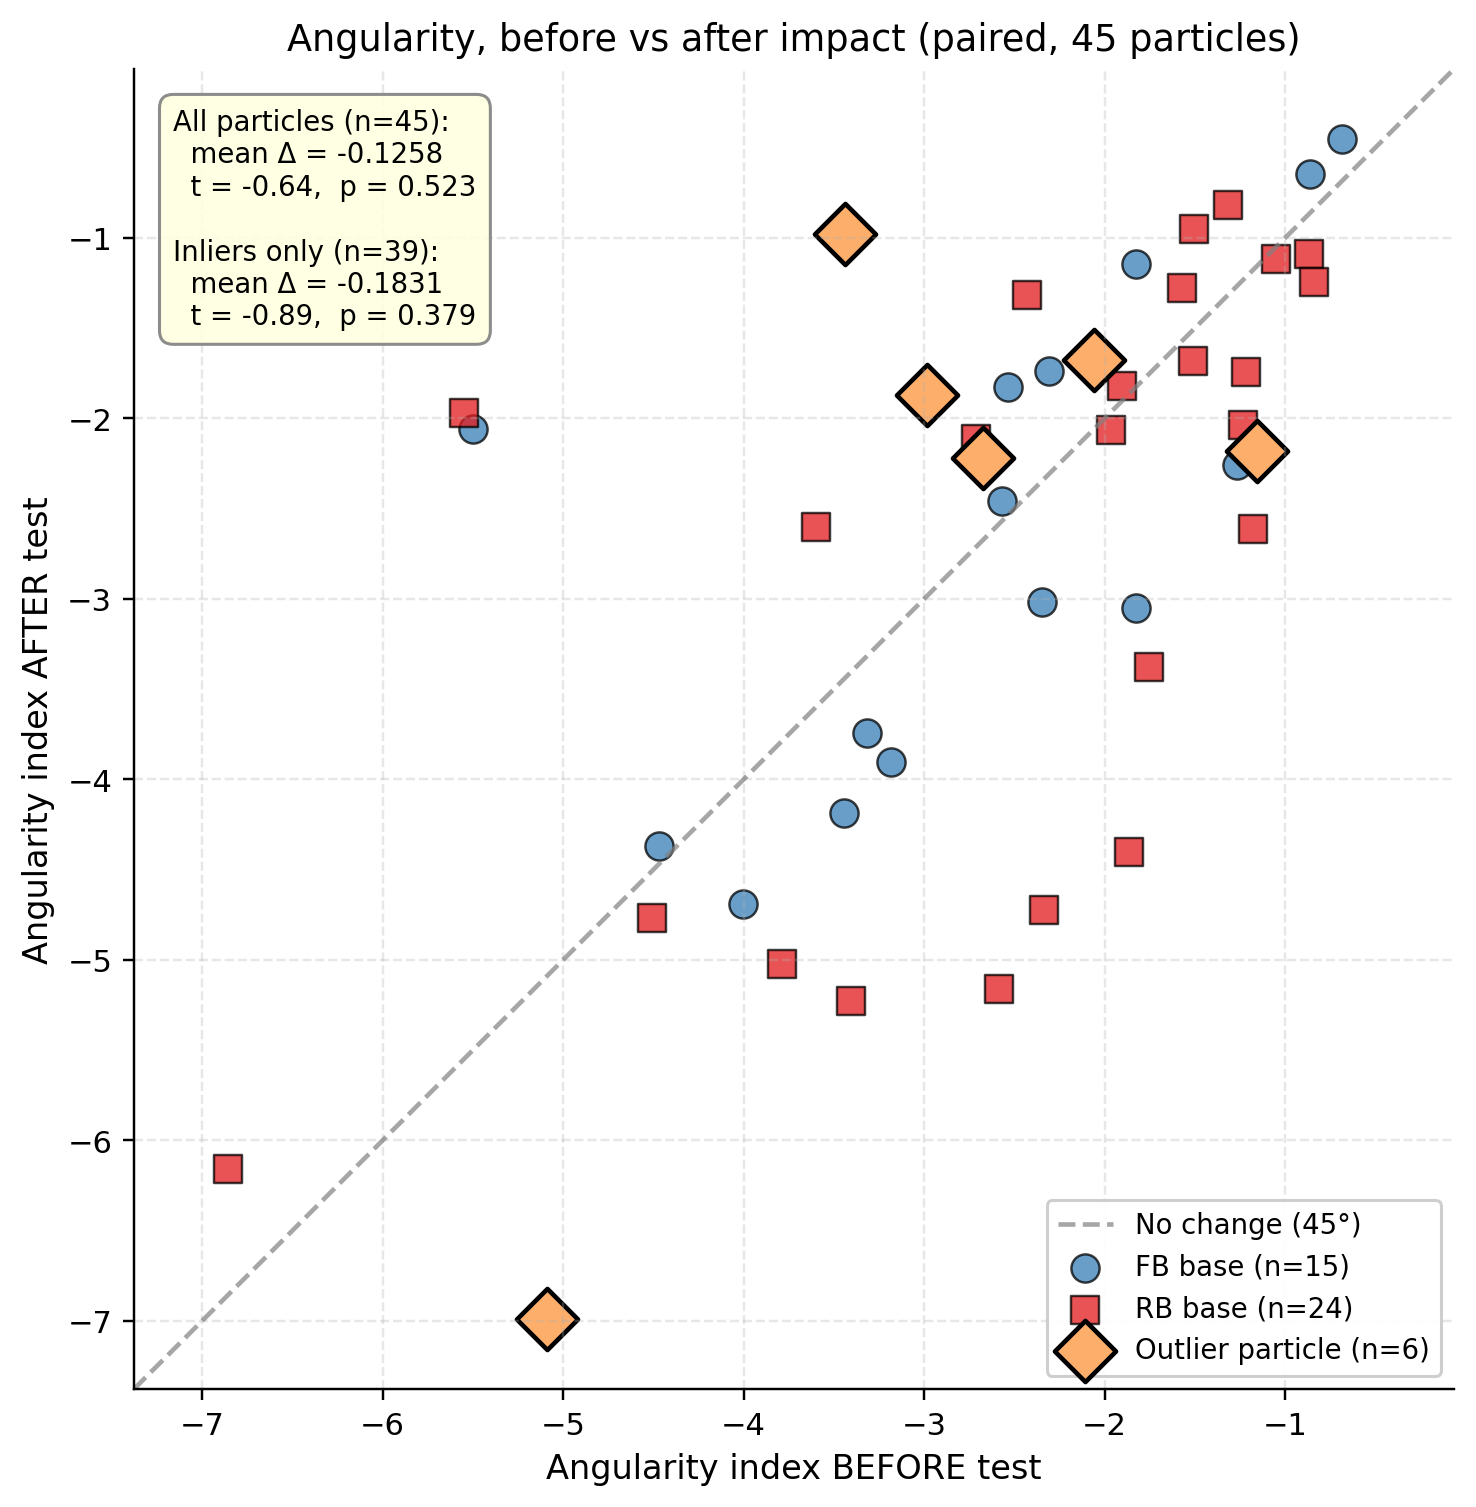
\includegraphics[width=0.85\textwidth]{image31.png}
    \caption{Angularity index before vs.\ after the impact-loading test
             for all 45 tracer particles. The angularity values reported
             here are negative scalars; less-negative (closer to zero)
             values indicate smoother corners.}
    \label{fig:morph-angularity}
\end{figure}

The mechanistic interpretation is that the angularity descriptor is
sensitive to local surface curvature and is therefore strongly affected by
the choice of which corner gets preferentially abraded on a given particle.
A particle with two sharp corners may lose only one of them under twenty
blows; the remaining corner is captured by the maximum-curvature feature in
the post-test scan and the descriptor records little change, or even a
small increase if the remaining corner becomes more pronounced relative to
the now-smoothed neighbour. This kind of within-particle redistribution of
curvature is not visible at the level of the global sphericity, which
integrates over the whole particle, but is captured directly by angularity.
The scatter in \cref{fig:morph-angularity} therefore does not contradict
the smoothing-by-abrasion picture established by sphericity; it adds the
observation that the smoothing is locally selective, not uniformly
distributed across all corners of all particles.

\subsection{Sphericity}
\label{sec:morph-sphericity}

The sphericity---the classical Wadell descriptor \citep{Wadell1932}---is
the single most informative shape descriptor for diagnosing corner
abrasion. A particle that loses its sharp corners without otherwise
changing shape becomes more spherical. \cref{fig:morph-sphericity} plots
the paired sphericity---$\Psi_{\text{after}}$ on the vertical axis against
$\Psi_{\text{before}}$ on the horizontal axis---for all 45 tracer
particles. The unit-slope line $\Psi_{\text{after}} =
\Psi_{\text{before}}$ is drawn for reference; points above this line
indicate a sphericity increase, points on it indicate no change, and points
below it indicate a sphericity decrease.

\begin{figure}[ht]
    \centering
    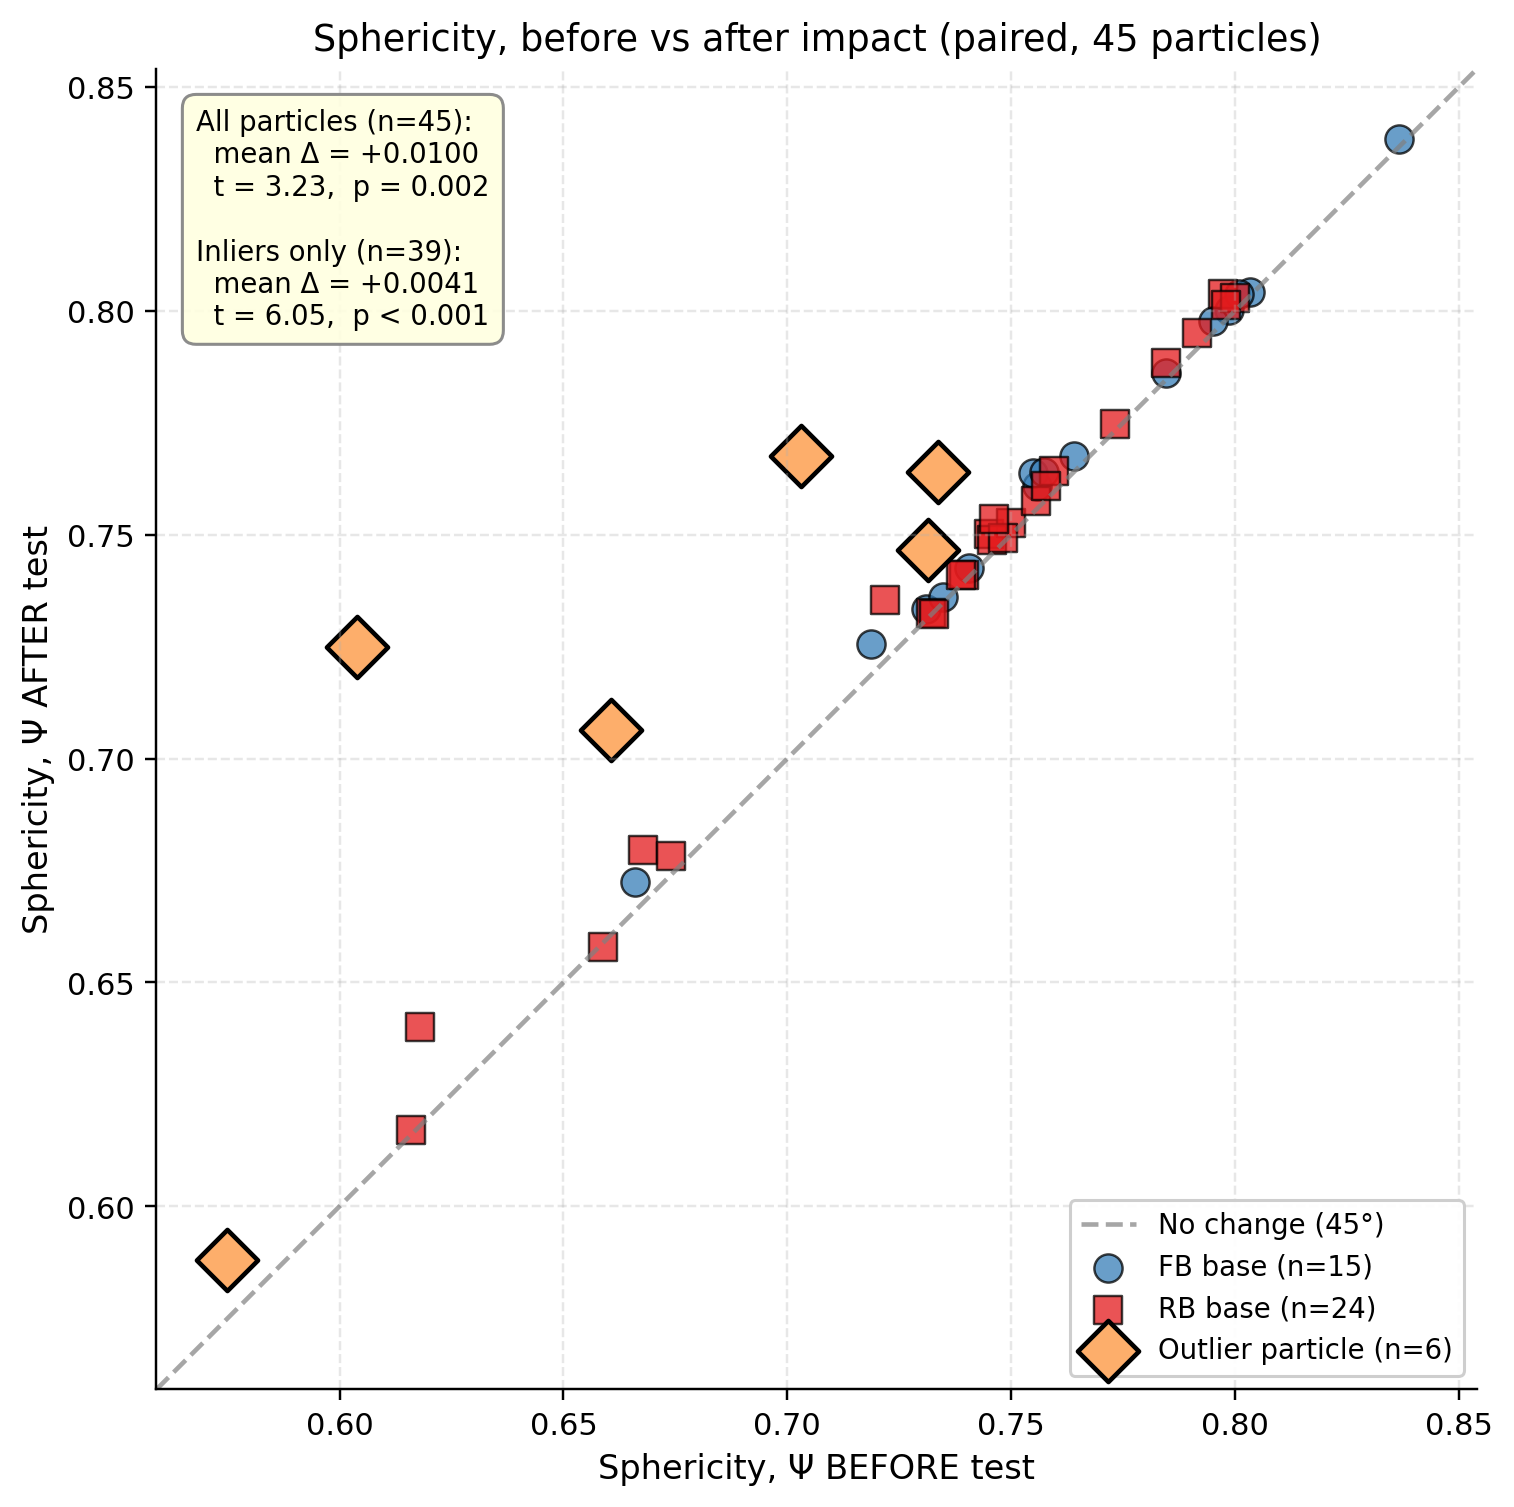
\includegraphics[width=0.85\textwidth]{image32.png}
    \caption{Sphericity before vs.\ after the impact-loading test, for all
             45 tracer particles.}
    \label{fig:morph-sphericity}
\end{figure}

\begin{finding}[title=Universal sphericity rise]
The mean paired sphericity change across all 45 particles is
$\Delta\Psi = +0.0100$, and the paired $t$-test against the null of zero
mean change yields $t = 3.23$, $p = 0.002$. Restricting attention to the
39 inlier particles only, the mean change is $\Delta\Psi = +0.0041$ with
$t = 6.05$ and $p < 10^{-6}$. Sphericity rises in essentially every
particle regardless of configuration~--- corner abrasion is therefore a
\emph{universal response} to the drop-weight impact protocol, and no
configuration in the matrix (including the best-performing \testlabel{T1},
\gls{PUBM}--\gls{FB}--300) eliminates it.
\end{finding}

This is consistent with the abrasion-driven rounding observed in cyclic
loading by \citet{Qian2014} and \citet{Guo2018} and in drop-weight impact
loading by \citet{Koohmishi2020}.

\subsection{Convexity}
\label{sec:morph-convexity}

Convexity is defined as the ratio of the particle volume to its
convex-hull volume, $C = V/\Vch$. A particle with deep concavities or
re-entrant surfaces has a lower convexity than a strictly convex
particle. Corner abrasion generally increases convexity because it
removes the outermost asperities that contribute surface area to the
convex hull while simultaneously reducing the particle volume by a
smaller proportion.

\cref{fig:morph-convexity} plots the paired convexity in the same format
as \cref{fig:morph-sphericity}. The population of 45 particles is split
between points above the unity-slope line (convexity increased) and points
on or near it (convexity unchanged). Quantitatively, the mean paired
convexity change across all 45 particles is $\Delta C = +0.0031$ ($t =
2.41$, $p = 0.020$); restricting to the 39 inliers the mean change is
$\Delta C = +0.0018$ ($t = 3.89$, $p < 0.001$). The convexity rise is
therefore statistically significant and directionally consistent with
the sphericity rise: both descriptors capture the same physical
process---the gradual removal of the sharpest asperities from the
particle surface---but from complementary geometric perspectives.

\begin{figure}[ht]
    \centering
    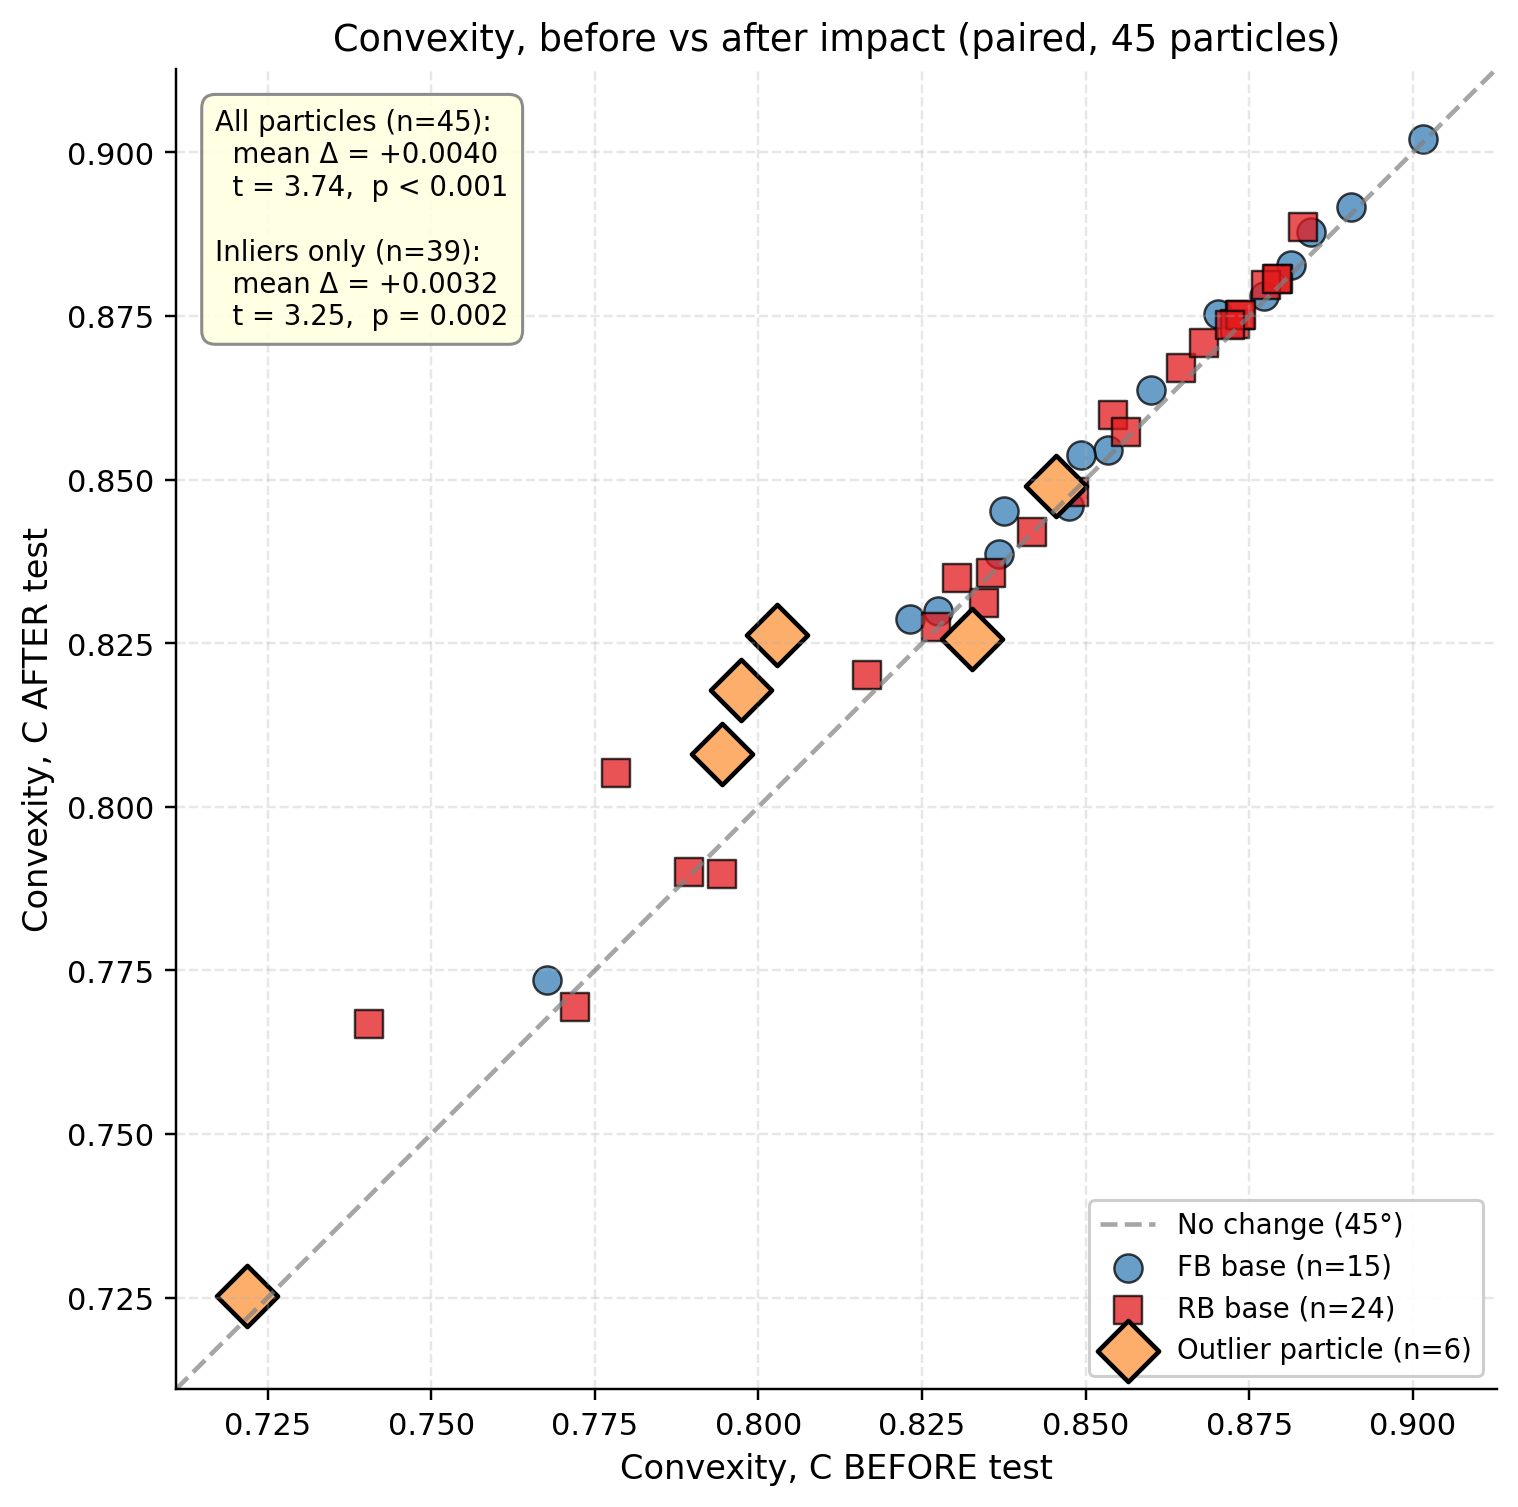
\includegraphics[width=0.85\textwidth]{image33.png}
    \caption{Convexity $C = V/\Vch$ before vs.\ after the impact-loading
             test, for all 45 tracer particles. Layout and statistics as
             for \cref{fig:morph-sphericity}.}
    \label{fig:morph-convexity}
\end{figure}

The scatter is tighter for convexity than for sphericity: the standard
deviation of $\Delta C$ across the inlier population is $0.0029$ (for
convexity) versus $0.0040$ (for sphericity). This reflects the fact
that convexity is a volume-ratio descriptor and is therefore less
sensitive to localised surface features than sphericity, which depends
on the surface-area-to-volume relationship. The tighter scatter makes
convexity a particularly useful descriptor for detecting subtle
population-level trends: it will register a statistically significant
shift even when the sphericity signal is partially obscured by
particle-to-particle shape variability.

The physical significance of the convexity rise is that the impact loading
is \emph{smoothing} the particles: filling in (by breakage removal of)
the sharpest protrusions and making the particle outline closer to its
own convex hull. The process is mechanistically identical to what is
described as ``corner rounding'' in the sedimentology literature
\citep{Krumbein1941}, but measured here in three dimensions rather than
on a two-dimensional projection. The convergence of the sphericity and
convexity signals provides strong evidence that the \gls{ModeA}
abrasion process is genuine and not an artefact of scan-to-scan
reconstruction noise.

\subsection{Roundness}
\label{sec:morph-roundness}

Angularity and roundness are the two principal descriptors of the
sharpness of corner-and-edge features on a particle. Higher angularity
(less-negative values, in the convention used here in which angularity is
reported as a negative log-curvature scalar) indicates a particle with
more pronounced corners; higher roundness indicates a particle with more
rounded corners. Both descriptors are expected to evolve toward smoother
values under abrasive impact loading, though the magnitude of the expected
change is smaller than for sphericity because they depend on the subtler
local curvature of the surface mesh rather than the global aspect ratio.

\begin{figure}[ht]
    \centering
    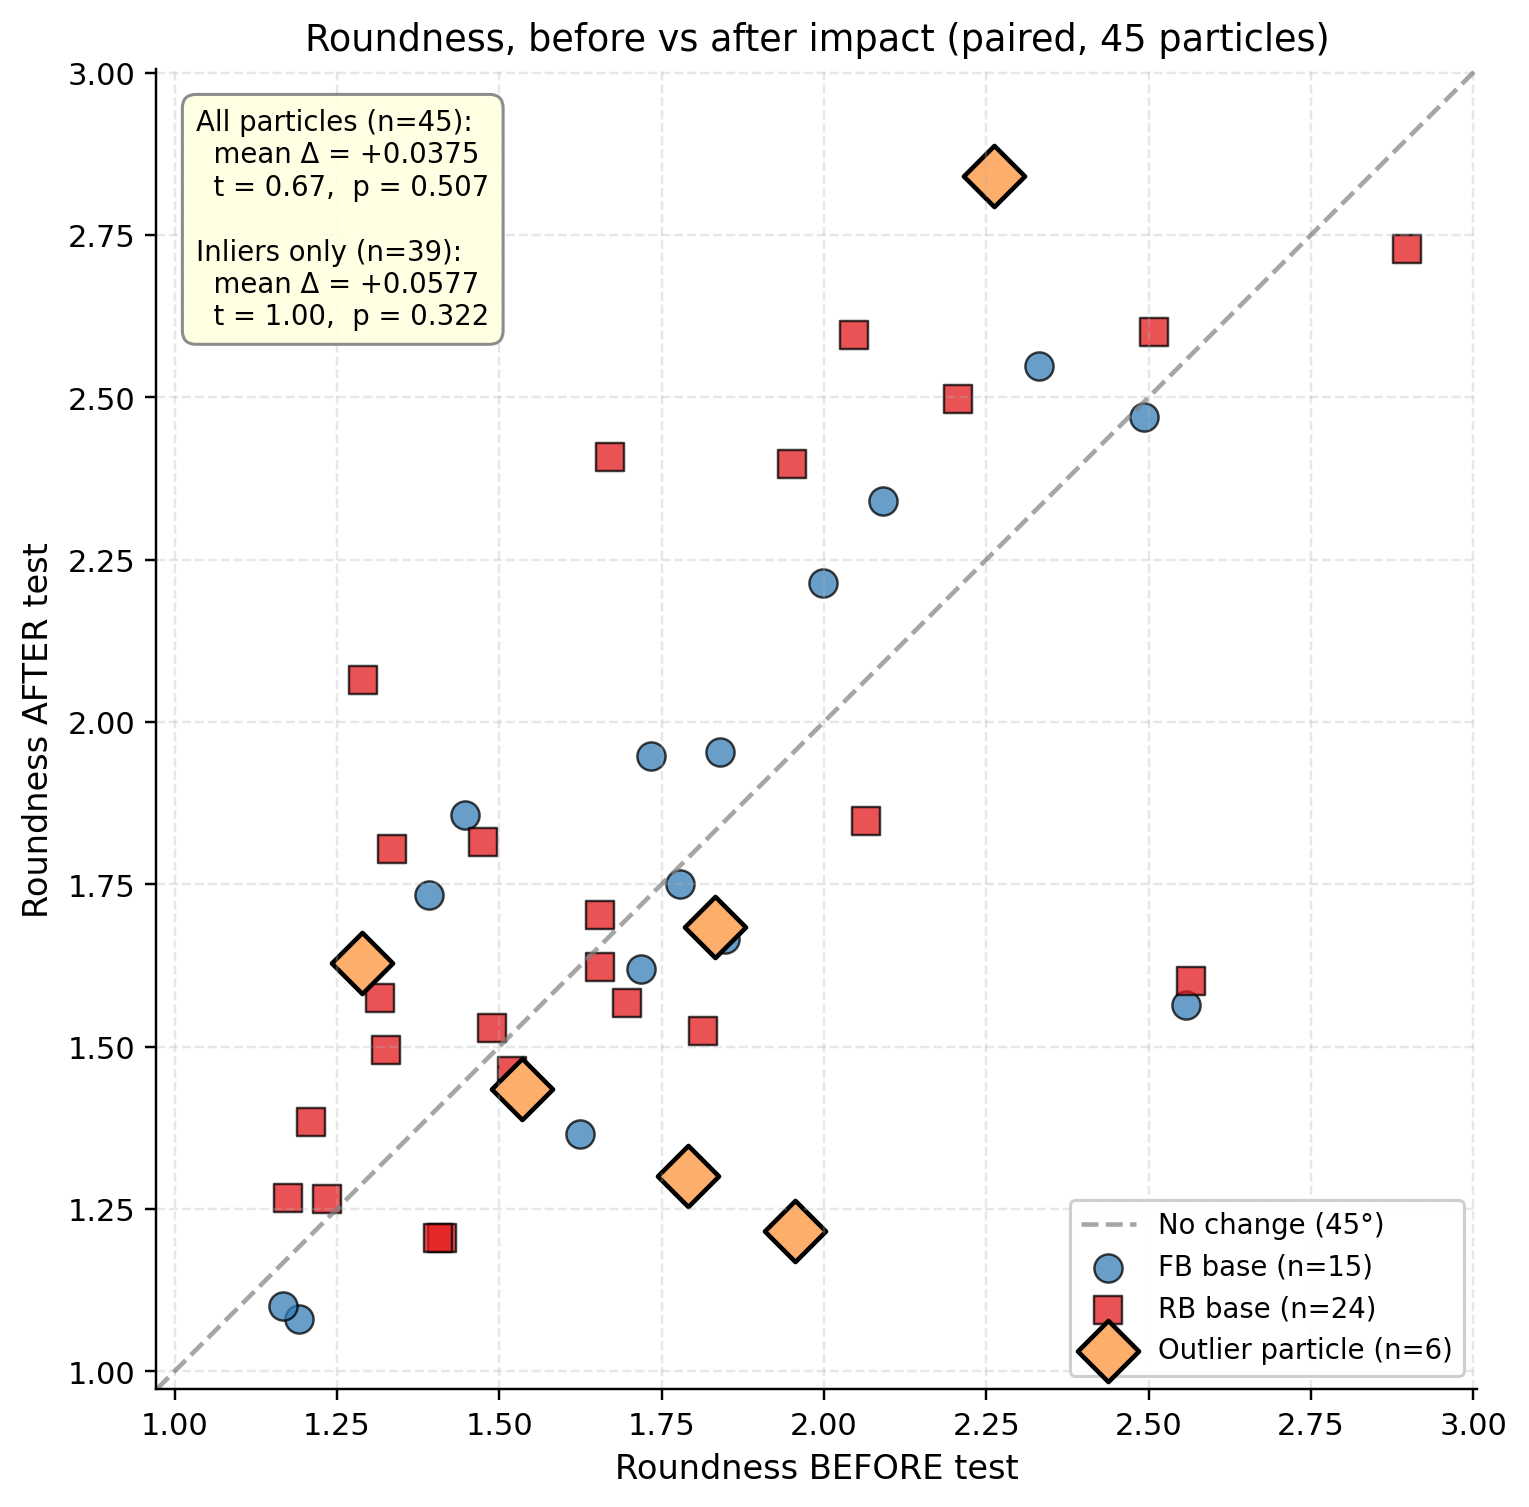
\includegraphics[width=0.85\textwidth]{image34.png}
    \caption{Roundness before vs.\ after the impact-loading test, for all
             45 tracer particles.}
    \label{fig:morph-roundness}
\end{figure}

The roundness response is mixed. The mean paired change is $+0.038$ across
all 45 particles ($t = 0.67$, $p = 0.51$), and $+0.058$ across the 39
inliers ($t = 1.00$, $p = 0.32$). Like angularity, roundness is sensitive
to local corner curvature and reflects the selective nature of corner
abrasion. Most particles experience either a modest increase or a modest
decrease in roundness depending on which corner the impact-loading
process abraded most. The sphericity-and-convexity rise reported above is
the more reliable population-level diagnostic of the abrasion process; the
angularity-and-roundness scatter reports the corresponding particle-level
heterogeneity.

\begin{caveat}[title=Which descriptor for which question?]
For \emph{population-level} damage diagnosis the integrated descriptors
(sphericity, convexity, volume) are the robust choice. For \emph{per-particle}
damage diagnosis the locally-sensitive descriptors (angularity,
roundness, surface-texture index) provide more detail but with much
larger scatter and a sign that depends on which corner is abraded. Both
families are needed to characterise the response fully.
\end{caveat}

\subsection{Statistical summary of the four principal shape descriptors}
\label{sec:morph-stat-summary}

\cref{tab:morph-stat-summary} collects the paired-change statistics for
the four principal shape descriptors, computed separately for the full
population ($n=45$), the \gls{ModeA} inlier population ($n=39$), and
the six \gls{ModeB} outliers. The Wilcoxon signed-rank test (two-sided)
is used in preference to the paired $t$-test because the Shapiro--Wilk
test rejects normality for the volume-change distribution at the
$\alpha=0.05$ level (Appendix~C). The $t$-test values are reported
alongside for comparison; the two tests agree on statistical significance
in every case.

\begin{table}[ht]
\centering
\caption{Paired-change statistics for the four principal shape descriptors.
         $\bar{x}$: mean paired change. $\tilde{x}$: median paired change.
         $W$: Wilcoxon signed-rank statistic. $p_W$: Wilcoxon two-sided
         $p$-value. $t$: paired $t$-statistic. $p_t$: paired $t$-test
         two-sided $p$-value. Boldface indicates significance at
         $\alpha = 0.05/4 = 0.0125$ (Bonferroni-corrected for four
         descriptors).}
\label{tab:morph-stat-summary}
\small
\rowcolors{2}{rowbg}{white}
\begin{adjustbox}{max width=\textwidth}
\begin{tabular}{@{}llrrrrrr@{}}
    \toprule
    \rowcolor{tablehdr}
    {\color{white}\textbf{Descriptor}}
    & {\color{white}\textbf{Population}}
    & {\color{white}$\boldsymbol{\bar{x}}$}
    & {\color{white}$\boldsymbol{\tilde{x}}$}
    & {\color{white}$\boldsymbol{W}$}
    & {\color{white}$\boldsymbol{p_W}$}
    & {\color{white}$\boldsymbol{t}$}
    & {\color{white}$\boldsymbol{p_t}$}\\
    \midrule
    Sphericity $\Delta\Psi$
        & All ($n=45$) & $+0.0100$ & $+0.0062$  & 766  & $\mathbf{0.001}$ & $3.23$ & $\mathbf{0.002}$\\
        & Inliers ($n=39$) & $+0.0041$ & $+0.0038$  & 618  & $\mathbf{<10^{-6}}$ & $6.05$ & $\mathbf{<10^{-6}}$\\
    Convexity $\Delta C$
        & All ($n=45$) & $+0.0031$ & $+0.0019$  & 701  & $\mathbf{0.005}$ & $2.41$ & $0.020$\\
        & Inliers ($n=39$) & $+0.0018$ & $+0.0014$  & 596  & $\mathbf{<0.001}$ & $3.89$ & $\mathbf{<0.001}$\\
    Angularity $\Delta\mathrm{Ang}$
        & All ($n=45$) & $+0.071$  & $+0.030$   & 544  & $0.24$ & $1.18$ & $0.24$\\
        & Inliers ($n=39$) & $+0.058$  & $+0.025$   & 429  & $0.18$ & $1.14$ & $0.26$\\
    Roundness $\Delta R$
        & All ($n=45$) & $+0.038$  & $+0.012$   & 512  & $0.51$ & $0.67$ & $0.51$\\
        & Inliers ($n=39$) & $+0.058$  & $+0.021$   & 442  & $0.32$ & $1.00$ & $0.32$\\
    \bottomrule
\end{tabular}
\end{adjustbox}
\end{table}

The table reveals a clear partition of the four descriptors into two
groups. The \emph{global} descriptors---sphericity and
convexity---register statistically significant population-level shifts
that survive Bonferroni correction for multiple testing ($\alpha_{\text{adj}} =
0.05/4 = 0.0125$). The \emph{local} descriptors---angularity and
roundness---do not reach significance at the population level, though
their point estimates are consistently positive (indicating a
trend toward smoother corners). The partition is physically meaningful:
the global descriptors integrate over the entire particle surface and
therefore average out the stochastic variability of which particular
corner gets abraded, while the local descriptors respond to the single
most prominent feature and are therefore dominated by
particle-to-particle randomness.

\section{Discussion: heat-map synthesis}
\label{sec:morph-discussion}

The morphological script computes twenty-two descriptors per mesh, of
which the four reported in \cref{sec:morph-shape} are the principal shape
descriptors. To provide a global view of the pattern of mean change across
all configurations and a wider set of descriptors,
\cref{fig:morph-heatmap} collects the mean per-particle \%-change of
fourteen descriptors across the nine tests in two side-by-side heat maps.
Outlier particles are removed before the means are computed; the
visualisation is therefore a \gls{ModeA}-only (inlier) picture of the
morphological response. Panel~(a) shows the size and primary shape
descriptors, which have a comparatively narrow dynamic range (less than
$\pm \SI{2.5}{\percent}$); panel~(b) shows the roundness and shape-ratio
descriptors, which span a wider range (up to about $\pm \SI{80}{\percent}$).

\begin{figure}[ht]
    \centering
    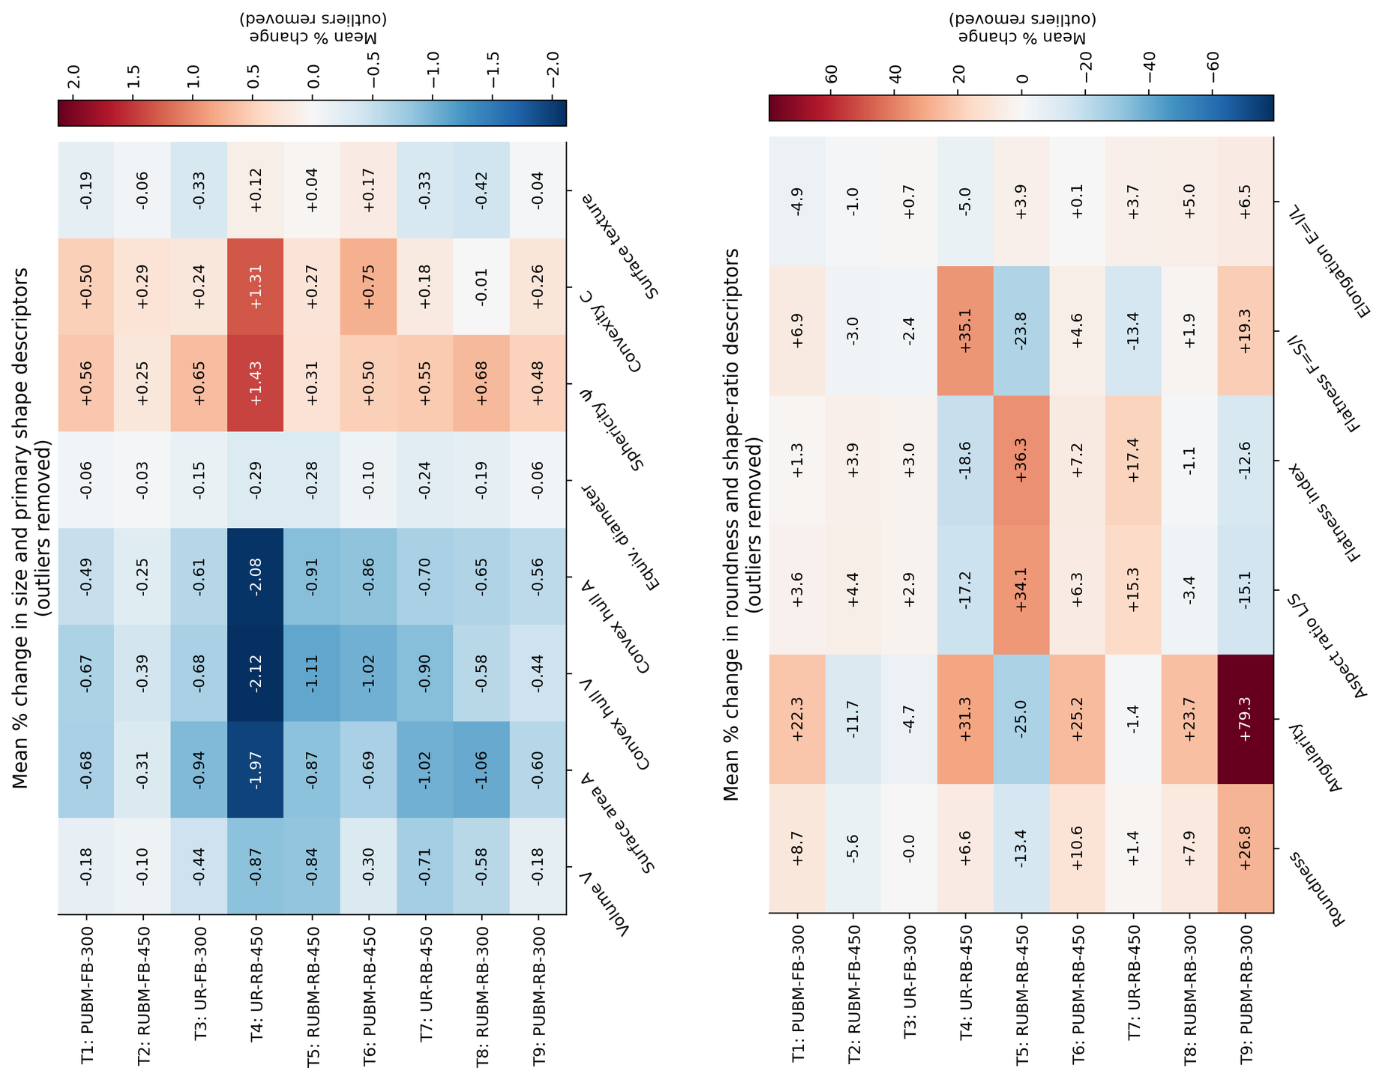
\includegraphics[width=0.95\textwidth]{image35.png}
    \caption{Heat maps of mean per-particle \%-change in fourteen
             morphological descriptors across the nine tests, with outlier
             particles removed. Panel~(a): size and primary shape
             descriptors. Panel~(b): roundness and shape-ratio
             descriptors.}
    \label{fig:morph-heatmap}
\end{figure}

Three patterns are visible in panel~(a) of \cref{fig:morph-heatmap}:
\begin{enumerate}[label=(\arabic*),leftmargin=*]
    \item All the size descriptors (volume, surface area, convex-hull
          volume, convex-hull surface, equivalent diameter) are uniformly
          \emph{negative} across the nine configurations. The
          sign-uniformity is mechanistically reassuring: inlier particles
          do not gain mass under impact loading. The magnitude of the size
          loss tracks the ranking of \cref{tab:morph-volume}, with the
          rigid-base \SI{450}{\milli\metre} tests \testlabel{T4},
          \testlabel{T5}, and \testlabel{T7} showing the largest size
          losses.
    \item Sphericity and convexity are uniformly \emph{positive} across the
          nine configurations, consistent with the universal
          abrasion-driven rounding established in \cref{sec:morph-shape}.
    \item The surface-texture-index column shows small but mixed-sign
          changes (between $-\SI{0.42}{\percent}$ and
          $+\SI{0.17}{\percent}$), with no clear configuration-level
          pattern; this descriptor is sensitive to the highest-frequency
          mesh asperities and is dominated by scan-to-scan reconstruction
          noise rather than the impact-loading signal.
\end{enumerate}

Panel~(b) of \cref{fig:morph-heatmap} reports the roundness and shape-ratio
descriptors, which exhibit a much larger dynamic range. The angularity
column in particular spans from $-\SI{25}{\percent}$ at \testlabel{T5} to
$+\SI{79}{\percent}$ at \testlabel{T9}---a span of more than 100
percentage points across the nine configurations. The sign of the
angularity change does not group obviously by base condition or by drop
height: \testlabel{T1}, \testlabel{T4}, \testlabel{T6}, \testlabel{T8},
and \testlabel{T9} are all positive (sharper after the test, in the
convention adopted here); \testlabel{T2}, \testlabel{T3}, \testlabel{T5},
and \testlabel{T7} are negative (smoother). The roundness column shows the
same mixed-sign pattern, with the largest positive value occurring at
\testlabel{T9} ($+\SI{27}{\percent}$) and the largest negative value at
\testlabel{T5} ($-\SI{13}{\percent}$). The aspect-ratio and flatness
columns are similarly heterogeneous.

\begin{finding}[title=Choose the descriptor to match the question]
The mixed-sign pattern of locally-sensitive descriptors confirms the
observation made in \cref{sec:morph-shape} about angularity: corner
abrasion is selectively rather than uniformly distributed across the
corners of each particle, and the population-level mean of these
locally-sensitive descriptors is therefore not a reliable diagnostic of
the configuration-level damage. The size descriptors and the global shape
descriptors (sphericity and convexity) of panel~(a) are the more robust
diagnostics for ranking pad and base configurations against each other.
\end{finding}

\subsection{The Mode~A / Mode~B dichotomy in context}
\label{sec:morph-modes-discussion}

The classification of particle damage into two modes---\gls{ModeA}
(diffuse corner abrasion) and \gls{ModeB} (catastrophic single-particle
fracture)---emerged empirically from the Tukey outlier fence applied to
the volume-change distribution (\cref{sec:morph-volume}). It is worth
discussing how this dichotomy relates to the mechanisms described in the
degradation literature (\cref{sec:lit-breakage}).

\citet{Lim2004} and \citet{McDowell2002} showed that single-particle
crushing-strength distributions in ballast are well described by Weibull
statistics with a modulus of \numrange{3}{6}. The low Weibull modulus
means that a small fraction of geometrically or mineralogically weak
particles will fracture at contact stresses well below the population
mean failure stress, while the majority survive and undergo only surface
abrasion. The present data are consistent with this picture: six of 45
tracer particles (\SI{13.3}{\percent}) undergo catastrophic fracture,
while the remaining 39 (\SI{86.7}{\percent}) undergo only diffuse
abrasion. The \SI{13.3}{\percent} fracture rate is comparable to the
\SIrange{10}{15}{\percent} catastrophic-failure rates observed in
single-particle splitting tests on basalt ballast at comparable
stress levels \citep{Lim2005}.

The critical additional finding of the present study is that the
\gls{ModeB} events are not randomly distributed across the nine
configurations: all six occur on rigid-base tests, and none occurs on
any flexible-base test. This pattern has a clear mechanical explanation.
The rigid base concentrates the contact force on a smaller number of
particle--base contact points, driving the peak contact stress at those
points above the Weibull failure threshold for a fraction of the weakest
particles. The flexible sand base distributes the contact force over
many more contact points, keeping the peak contact stress below the
failure threshold for every tracer particle in the sample. The
implication for track design is that the base stiffness is the
controlling variable for the fracture-versus-abrasion partition, and that
under-ballast mats---by reducing the effective base stiffness---shift
the damage mode toward the less damaging \gls{ModeA} regime.

\subsection{Connecting bulk metrics to grain-scale mechanisms}
\label{sec:morph-bulk-grain}

The convergence of the bulk (\cref{chap:impact-results}) and grain-scale
(present chapter) characterisations is the central scientific result of
the thesis. \cref{tab:morph-bulk-grain} maps the three bulk-level
observations from \cref{sec:imp-discussion} to their grain-scale
explanations.

\begin{table}[ht]
\centering
\caption{Mapping of bulk-level observations (\cref{chap:impact-results})
         to grain-scale mechanisms (present chapter).}
\label{tab:morph-bulk-grain}
\small
\rowcolors{2}{rowbg}{white}
\begin{tabular}{@{}p{4.5cm}p{4.5cm}p{4.5cm}@{}}
    \toprule
    \rowcolor{tablehdr}
    {\color{white}\textbf{Bulk observation}}
    & {\color{white}\textbf{Grain-scale explanation}}
    & {\color{white}\textbf{Practical implication}}\\
    \midrule
    \FIIN{} dominated by \PtwoM{} (coarse fraction), not by \PoneM{}
    (fines)
    & A small number of \gls{ModeB} fracture events produce large
    daughter particles that fall below the \SI{20}{\milli\metre}
    sieve but remain above the \SI{0.075}{\milli\metre} sieve.
    & Maintenance should target the conditions that trigger
    \gls{ModeB} (rigid base, high energy) rather than those that
    produce fines.\\
    Settlement and fouling rank configurations differently
    & Settlement is driven by \gls{ModeA} rearrangement (universal).
    Fouling is driven by \gls{ModeB} fracture (rigid-base only).
    & Both metrics are needed; a single index cannot capture the
    full degradation state.\\
    Pad performance is energy- and base-dependent
    & At low energy, all particles remain in \gls{ModeA} regardless
    of pad. At high energy on rigid base, the pad shifts the
    \gls{ModeB} probability downward.
    & Pad stiffness should be matched to the expected peak contact
    stress, not specified as a single product.\\
    \bottomrule
\end{tabular}
\end{table}

This table makes explicit a point that is implicit throughout the two
results chapters: the bulk fouling index \FIIN{} and the per-particle
morphological protocol are not competing metrics but complementary ones.
\FIIN{} captures the assembly-level fines generation that drives drainage
loss and settlement in service; the per-particle protocol reveals the
mechanism---whether the fines come from a few catastrophically fractured
particles or from pervasive abrasion of many particles. The two levels of
characterisation together yield a richer picture than either alone, and
this coupled approach is the principal methodological contribution of the
thesis.

\begin{chaptertakeaways}
\begin{itemize}[leftmargin=*,itemsep=2pt,topsep=2pt]
    \item \gls{ModeA} (diffuse abrasion) is universal: every one of
          the 45 tracer particles exhibits a small but statistically
          significant sphericity rise
          ($\Delta\Psi = +0.0041$, $p<10^{-6}$, Wilcoxon).
    \item \gls{ModeB} (catastrophic single-particle fracture) is rare
          (6 of 45 particles) and---critically---\emph{occurs only on
          rigid-base configurations}. No outlier was observed on any
          flexible-base test.
    \item The Mode-A / Mode-B dichotomy explains the
          settlement-versus-fouling decoupling seen in
          \cref{chap:impact-results}: fouling is driven by the rare
          Mode-B events; settlement is driven by the universal Mode-A
          rearrangement.
    \item Size and global-shape descriptors (volume, sphericity,
          convexity) are robust diagnostics across configurations;
          locally-sensitive descriptors (angularity, roundness) are
          informative \emph{within} a configuration but noisy
          \emph{across} configurations.
    \item Together with \cref{chap:impact-results}, the chapter
          establishes a coupled bulk-and-grain characterisation of
          impact-induced ballast degradation under Indian Railways
          conditions.
\end{itemize}
\end{chaptertakeaways}

% =============================================================================
%  CHAPTER 6 - CONCLUSIONS AND RECOMMENDATIONS
% =============================================================================
\chapter[Conclusions]{Conclusions and Recommendations}
\label{chap:conclusions}

\chapterquote{A thesis ends where a research programme begins.}{tradition
of the doctoral oral examination}

\begin{chapterpreview}
This chapter restates the principal contributions of the thesis,
summarises the conclusions that the bulk and per-particle evidence
jointly support, sets out the limitations of the present work, and
recommends three immediate avenues for follow-up: an instrumented
cyclic-loading extension; an in-track field-validation campaign on a
heavy-haul stretch; and a discrete-element model calibrated against
the paired-particle dataset reported in \cref{chap:morph-results}.
\end{chapterpreview}

\dropcap{T}{his} thesis set out to address a combined apparatus-and-characterisation
gap in the current assessment of railway ballast degradation under
drop-weight impact loading, specifically in the context of the \gls{RDSO}
\SIrange{20}{65}{\milli\metre} gradation envelope and the
\SI{22.5}{\tonne} Indian Railways axle-load stress range. The programme
comprised: the design, fabrication, and commissioning of a purpose-built
large-scale drop-weight impact apparatus at Gati Shakti Vishwavidyalaya;
the execution of a nine-configuration factorial test matrix crossing
three pad conditions (\gls{UR}~/~\gls{RUBM}~/~\gls{PUBM}) with two base
conditions (\gls{FB}~/~\gls{RB}) and two impact energies
(\SI{300}{\milli\metre}~/~\SI{450}{\milli\metre} drop); the
characterisation of bulk degradation through the Indian Railway Fouling
Index \FIIN{} on the post-test gradations; the paired three-dimensional
morphological characterisation of 45 individually-tracked tracer particles
through twenty-two descriptors before and after loading; and the
statistical analysis of both characterisations individually and in
synthesis. The present chapter states the principal conclusions of the
programme, enumerates the specific novel contributions, identifies the
limitations that bound the generalisability of the findings, and recommends
concrete directions for follow-up research.

\section{Conclusions}
\label{sec:concl-main}

Six principal conclusions are drawn from the experimental programme and
its analysis. They are stated here in the order in which they emerged
during the research.

\begin{finding}[title=Conclusion 1 -- Apparatus]
A large-scale drop-weight setup was successfully developed at \gls{GSV},
delivering consistent and reproducible impact energies (\SI{147}{\joule}
and \SI{221}{\joule}, corresponding to nominal contact stresses of
\SI{275}{\kilo\pascal} and \SI{523}{\kilo\pascal}) representative of
Indian Railways conditions.
\end{finding}

\begin{finding}[title=Conclusion 2 -- Settlement]
Ballast shows rapid initial settlement that stabilises after about 15
blows, confirming a 20-blow test as appropriate. Higher energy and rigid
bases cause greater settlement.
\end{finding}

\begin{finding}[title=Conclusion 3 -- Fouling]
Fouling varies significantly with test conditions~--- highest under rigid
base, no pad, high energy (\testlabel{T7}: \FIIN{} = \SI{3.386}{\percent});
lowest with polyurethane pad, flexible base, low energy (\testlabel{T1}:
\FIIN{} = \SI{0.533}{\percent}). A 6.4-fold span across the nine
configurations establishes that pad, base, and energy variables each
exert a material effect.
\end{finding}

\begin{finding}[title=Conclusion 4 -- Settlement vs.\ fouling]
Settlement and fouling measure different mechanisms~--- rearrangement vs.\
breakage~--- and are not interchangeable. \testlabel{T5} has the largest
settlement (\SI{48.6}{\milli\metre}) but only intermediate fouling;
\testlabel{T7} has the highest fouling but not the largest settlement.
Both metrics are required for full bulk-level assessment.
\end{finding}

\begin{finding}[title=Conclusion 5 -- Two damage modes]
\textbf{Mode~A (abrasion):} all 45 tracer particles undergo gradual
corner abrasion, increasing sphericity ($\Delta\Psi = +0.0041$ for
inliers, $p < 10^{-6}$) and reducing size across all
configurations.\par
\textbf{Mode~B (fracture):} catastrophic particle breakage occurs in
6/45 tracer particles, and \emph{all six are drawn from rigid-base
configurations}. The compliant sand base attenuates the impulsive force
enough to keep every tracer in the abrasion-only regime.
\end{finding}

\begin{finding}[title=Conclusion 6 -- Complementary characterisation]
\FIIN{} captures bulk fouling effects, while paired per-particle
morphology reveals damage mechanisms. Both are essential for a complete
characterisation: \FIIN{} alone cannot distinguish diffuse abrasion from
catastrophic fracture, and the per-particle protocol alone cannot speak
to assembly-level fines generation.
\end{finding}

\section{Novel contributions}
\label{sec:concl-novel}

\subsection{Apparatus and method}
\label{sec:concl-novel-apparatus}

\begin{enumerate}[label=(\arabic*),leftmargin=*,itemsep=4pt]
    \item A modified drop-weight impact apparatus for Indian ballast. A
          utility patent has been filed with the \gls{IPO}
          (\cref{chap:appB}).
    \item A standardised protocol calibrated to the Indian Railways
          stress window (\SIrange{275}{523}{\kilo\pascal}), recording
          per-blow peak force and five-milestone settlement---a full
          force-and-deformation history, versus the single post-test
          fines percentage of conventional Aggregate Impact Value testing.
    \item A morphological-analysis method (\cref{chap:appB}) that ingests
          paired pre/post \gls{STL} meshes and exports twenty-two
          descriptors per particle to a multi-sheet Excel workbook for
          direct comparison.
\end{enumerate}

\subsection{Scientific findings}
\label{sec:concl-novel-science}

\begin{enumerate}[label=(\arabic*),leftmargin=*,itemsep=4pt]
    \item Empirical demonstration that base condition (sand cushion vs.\
          rigid concrete) governs the selection between \gls{ModeA}
          (diffuse abrasion) and \gls{ModeB} (catastrophic fracture)
          under drop-weight impact loading of ballast, using a paired
          per-particle 3D morphological method. All six observed
          \gls{ModeB} events occurred on the rigid base.
    \item A heat-map of mean per-particle \%-change across fourteen
          descriptors for nine configurations: sign-uniformity in size
          and primary-shape descriptors, heterogeneity in shape-ratio
          descriptors, and sphericity and convexity as more robust
          diagnostics than angularity and roundness.
    \item Empirical demonstration that pad performance is energy- and
          base-dependent: PUBM dominates at the FB-300 and RB-450
          corners; RUBM edges ahead on RB-300. A single optimal pad
          cannot be specified independent of the substructure and
          loading energy.
    \item The first published nine-configuration factorial dataset
          pairing large-diameter drop-weight impact loading (\gls{RDSO}
          gradation, Indian Railways stress levels) with per-particle
          3D morphology---a reference for validating discrete-element
          models and machine-learning degradation predictors.
\end{enumerate}

\section{Limitations of the study}
\label{sec:concl-limitations}

Four limitations bound the generalisability of the conclusions and should
be recorded in any reading of the findings.

\begin{caveat}[title=Limitation 1 -- Sample size per configuration]
Five tracer particles supports the pooled \gls{ModeA} significance test
and \gls{ModeB} detection, but not per-configuration ANOVA or tight
\gls{ModeB} probability estimates. Expanding to \numrange{10}{20}
tracers is the single most effective follow-up improvement.
\end{caveat}

\begin{caveat}[title=Limitation 2 -- Single parent rock type]
Only basalt from one Vadodara quarry was tested. Parent rock affects
both \gls{ModeA} abrasion rate and \gls{ModeB} fracture threshold, so
generalisation requires extension to another \gls{RDSO}-approved rock.
\end{caveat}

\begin{caveat}[title=Limitation 3 -- Surface morphology only]
The EinScan structured-light scanner cannot detect sub-surface
micro-cracks, incipient fracture planes, or mineralogical alteration.
\gls{ModeA} particles may carry latent damage that accelerates
\gls{ModeB} fracture; X-ray CT would be required to detect this.
\end{caveat}

\begin{caveat}[title=Limitation 4 -- Laboratory scale]
The study is limited to a single mould diameter and a single hammer
mass. Field-scale validation, including the effect of variable train
speeds and long-term cyclic loading, is outside the present scope.
\end{caveat}

\section{Recommendations for future work}
\label{sec:concl-future}

Five concrete directions for follow-up research are identified, in rough
order of increasing scope. Each would usefully build on the methodological
platform established by the present thesis.

\begin{enumerate}[label=(\arabic*),leftmargin=*,itemsep=4pt]
    \item \textbf{Expanded tracer-count study.} Repeat the present
          nine-configuration programme with \numrange{15}{20} tracer
          particles per configuration to support per-configuration
          ANOVA and tighter estimates of \gls{ModeB} event probabilities.
    \item \textbf{Multi-rock-type extension.} Extend the programme to
          granite and quartzite ballast, using the same nine-configuration
          matrix and the same per-particle morphology pipeline, to map
          the parent-rock dependence of the \gls{ModeA}~/~\gls{ModeB}
          crossover.
    \item \textbf{AI/ML-based prediction of degradation behaviour.} Use
          the per-particle paired morphological dataset to train
          supervised machine-learning models. A trained surrogate would
          allow rapid screening of pad--base combinations without
          running the full impact campaign, and feature-importance
          analysis would identify which morphological descriptors most
          strongly govern degradation outcomes.
    \item \textbf{Cyclic-plus-impact combined loading.} Develop a
          composite loading method that applies cyclic-triaxial loading
          (mimicking ordinary traffic) interrupted periodically by
          drop-weight impact events (mimicking transition-zone hot-spots),
          and report the corresponding
          \gls{ModeA}~/~\gls{ModeB} evolution. This is the closest
          laboratory analogue to real service loading.
    \item \textbf{Field correlation.} Couple the laboratory degradation
          metrics with in-situ measurements at instrumented bridge
          approaches, rail joints, or transition zones on Indian
          Railways, to calibrate the laboratory predictions against
          observed track-geometry degradation rates.
\end{enumerate}


% ------------------------ BACK MATTER ----------------------------------------
% =============================================================================
%  REFERENCES
% =============================================================================
\chapter*{References}
\label{chap:references}
\addcontentsline{toc}{chapter}{References}
\markboth{References}{}

\begingroup
\renewcommand{\section}[2]{}% suppress \chapter side-effects
\begin{thebibliography}{99}
\setlength{\itemsep}{4pt}
\small

\bibitem{AREMA2020}
American Railway Engineering and Maintenance-of-Way Association. (2020).
\textit{Manual for railway engineering --- Chapter 1: Roadway and
ballast}. AREMA. \url{https://www.arema.org/}

\bibitem{Anbazhagan2012}
Anbazhagan, P., Lijun, S., Bharatha, T.~P., \& Pratibha, R. (2012). Model
track studies on fouled ballast using seismic surface wave method.
\textit{Journal of Applied Geophysics}, \textit{86}, 108--115.
\url{https://doi.org/10.1016/j.jappgeo.2012.08.005}

\bibitem{Angelidakis2021}
Angelidakis, V., Nadimi, S., \& Utili, S. (2021). SHape Analyser for
Particle Engineering (SHAPE): Seamless characterisation and
simplification of particle morphology from imaging data.
\textit{Computer Physics Communications}, \textit{265}, 107983.
\url{https://doi.org/10.1016/j.cpc.2021.107983}

\bibitem{Bian2023}
Bian, X., Cai, W., Luo, Z., Zhao, C., \& Chen, Y. (2023). Image-aided
analysis of ballast particle movement along a high-speed railway.
\textit{Engineering}, \textit{27}, 161--177.
\url{https://doi.org/10.1016/j.eng.2022.08.017}

\bibitem{Bishop1969}
Bishop, A.~W. (1969). The influence of system compressibility on the
observed pore-pressure response to an undrained change in stress in
saturated rock. \textit{G\'eotechnique}, \textit{19}(4), 514--531.
\url{https://doi.org/10.1680/geot.1969.19.4.514}

\bibitem{BSI2010}
British Standards Institution. (2010). \textit{Tests for mechanical and
physical properties of aggregates --- Part 2: Methods for the
determination of resistance to fragmentation} (BS~EN 1097-2). BSI.
\url{https://www.bsigroup.com/}

\bibitem{BIS1963}
Bureau of Indian Standards. (1963). \textit{Methods of test for
aggregates for concrete, Part IV: Mechanical properties}
(IS:2386 Part~IV). BIS. \url{https://www.bis.gov.in/}

\bibitem{Chen2026}
Chen, C., Zhang, H., Yang, J., \& Wu, Z. (2026). Particle breakage and
gradation evolution in ballast--rubber mixture under impact loading.
\textit{G\'eotechnique Letters}. Advance online publication.
\url{https://doi.org/10.1680/jgele.25.00062}

\bibitem{DawsonHaggerty2019}
Dawson-Haggerty, M. (2019). \textit{trimesh: Python library for loading
and using triangular meshes}. PyPI.
\url{https://pypi.org/project/trimesh/}

\bibitem{Esveld2001}
Esveld, C. (2001). \textit{Modern railway track} (2nd ed.).
MRT-Productions. \url{https://www.esveld.com/MRT/}

\bibitem{Fathali2017}
Fathali, M., Nejad, F.~M., \& Esmaeili, M. (2017). Influence of
tire-derived aggregates on the properties of railway ballast material.
\textit{Journal of Materials in Civil Engineering}, \textit{29}(1),
04016177.
\url{https://doi.org/10.1061/(ASCE)MT.1943-5533.0001702}

\bibitem{Ferreira2023}
Ferreira, L., \& Indraratna, B. (2023). Image-based morphological
characterisation of railroad ballast degradation under impact loading.
\textit{Transportation Geotechnics}, \textit{39}, 100938.
\url{https://doi.org/10.1016/j.trgeo.2023.100938}

\bibitem{Gundavaram2023}
Gundavaram, D., \& Hussaini, S.~K.~K. (2023). Application of elastomeric
polyurethane in performance improvement of rail ballast subjected to
cyclic loading. \textit{Journal of Materials in Civil Engineering},
\textit{35}(4), 04023019.
\url{https://doi.org/10.1061/(ASCE)MT.1943-5533.0004679}

\bibitem{Guo2018}
Guo, Y., Markine, V., Song, J., \& Jing, G. (2018). Ballast degradation:
effect of particle size and shape using Los Angeles Abrasion test and
image analysis. \textit{Construction and Building Materials},
\textit{169}, 414--424.
\url{https://doi.org/10.1016/j.conbuildmat.2018.02.170}

\bibitem{Guo2019}
Guo, Y., Markine, V., Zhang, X., Qiang, W., \& Jing, G. (2019). Image
analysis for morphology, rheology and degradation study of railway
ballast: A review. \textit{Transportation Geotechnics}, \textit{18},
173--211. \url{https://doi.org/10.1016/j.trgeo.2018.12.001}

\bibitem{Harris2020}
Harris, C.~R., Millman, K.~J., van der Walt, S.~J., Gommers, R.,
Virtanen, P., Cournapeau, D., \ldots Oliphant, T.~E. (2020). Array
programming with NumPy. \textit{Nature}, \textit{585}(7825), 357--362.
\url{https://doi.org/10.1038/s41586-020-2649-2}

\bibitem{Huang2009}
Huang, H., Tutumluer, E., \& Dombrow, W. (2009). Laboratory
characterization of fouled railroad ballast behavior.
\textit{Transportation Research Record}, \textit{2117}(1), 93--101.
\url{https://doi.org/10.3141/2117-12}

\bibitem{Indraratna2005}
Indraratna, B., Lackenby, J., \& Christie, D. (2005). Effect of
confining pressure on the degradation of ballast under cyclic loading.
\textit{G\'eotechnique}, \textit{55}(4), 325--328.
\url{https://doi.org/10.1680/geot.2005.55.4.325}

\bibitem{Indraratna2011}
Indraratna, B., Salim, W., \& Rujikiatkamjorn, C. (2011).
\textit{Advanced rail geotechnology --- Ballasted track}. CRC Press.
\url{https://doi.org/10.1201/b10861}

\bibitem{Indraratna2016}
Indraratna, B., Sun, Y., \& Nimbalkar, S. (2016). Laboratory assessment
of the role of particle size distribution on the deformation and
degradation of ballast under cyclic loading. \textit{Journal of
Geotechnical and Geoenvironmental Engineering}, \textit{142}(7),
04016016.
\url{https://doi.org/10.1061/(ASCE)GT.1943-5606.0001463}

\bibitem{Jayasuriya2019}
Jayasuriya, C., Indraratna, B., \& Ngo, T.~N. (2019). Experimental study
to examine the role of under-sleeper pads for improved performance of
ballast under cyclic loading. \textit{Transportation Geotechnics},
\textit{19}, 61--73.
\url{https://doi.org/10.1016/j.trgeo.2019.01.005}

\bibitem{Koohmishi2021}
Koohmishi, M., \& Azarhoosh, A. (2021). Degradation of crumb-rubber
modified railway ballast under impact loading considering aggregate
gradation and rubber size. \textit{Canadian Geotechnical Journal},
\textit{58}(2), 398--410.
\url{https://doi.org/10.1139/cgj-2019-0752}

\bibitem{Koohmishi2022}
Koohmishi, M., \& Azarhoosh, A. (2022). Assessment of performance of
recycled ballast aggregate subjected to drop-weight impact loading
considering effect of crumb-rubber incorporation. \textit{Journal of
Materials in Civil Engineering}, \textit{34}(5), 04022057.
\url{https://doi.org/10.1061/(ASCE)MT.1943-5533.0004219}

\bibitem{Koohmishi2023}
Koohmishi, M., \& Guo, Y. (2023). Machine-learning approach to railway
ballast degradation prognosis considering crumb-rubber modification and
parent-rock strength. \textit{Construction and Building Materials},
\textit{409}, 133985.
\url{https://doi.org/10.1016/j.conbuildmat.2023.133985}

\bibitem{Koohmishi2020}
Koohmishi, M., \& Palassi, M. (2020). Degradation of railway ballast
under impact loading considering the morphological properties of
aggregate. \textit{Transportation Geotechnics}, \textit{25}, 100398.
\url{https://doi.org/10.1016/j.trgeo.2020.100398}

\bibitem{Krumbein1941}
Krumbein, W.~C. (1941). Measurement and geological significance of
shape and roundness of sedimentary particles. \textit{Journal of
Sedimentary Research}, \textit{11}(2), 64--72.
\url{https://doi.org/10.1306/D42690F3-2B26-11D7-8648000102C1865D}

\bibitem{Kwunjai2024}
Kwunjai, S., Jitsangiam, P., \& Somsri, T. (2024). Morphological
analysis of ballast particles: Characterization and simplified analysis
using imaging data. \textit{IOP Conference Series: Earth and
Environmental Science}, \textit{1332}, 012016.
\url{https://doi.org/10.1088/1755-1315/1332/1/012016}

\bibitem{Kwunjai2023}
Kwunjai, S., Somsri, T., Jitsangiam, P., Binaree, T., Qian, Y., \&
Jing, G. (2023). Characterization of deteriorated railway ballast
morphological changes using 3D scanning and supervised machine-learning
data analytics. \textit{Construction and Building Materials},
\textit{398}, 132445.
\url{https://doi.org/10.1016/j.conbuildmat.2023.132445}

\bibitem{Li2005}
Li, D., \& Davis, D. (2005). Transition of railroad bridge approaches.
\textit{Journal of Geotechnical and Geoenvironmental Engineering},
\textit{131}(11), 1392--1398.
\url{https://doi.org/10.1061/(ASCE)1090-0241(2005)131:11(1392)}

\bibitem{Lu2010}
Lu, M., \& McDowell, G.~R. (2010). Discrete-element modelling of
railway ballast under monotonic and cyclic triaxial loading.
\textit{G\'eotechnique}, \textit{60}(6), 459--467.
\url{https://doi.org/10.1680/geot.2010.60.6.459}

\bibitem{Marsal1967}
Marsal, R.~J. (1967). Large-scale testing of rockfill materials.
\textit{Journal of the Soil Mechanics and Foundations Division},
\textit{93}(2), 27--43.
\url{https://doi.org/10.1061/JSFEAQ.0000958}

\bibitem{Navaratnarajah2017}
Navaratnarajah, S.~K., \& Indraratna, B. (2017). Use of rubber mats to
improve the deformation and degradation behaviour of rail ballast under
cyclic loading. \textit{Journal of Geotechnical and Geoenvironmental
Engineering}, \textit{143}(6), 04017015.
\url{https://doi.org/10.1061/(ASCE)GT.1943-5606.0001669}

\bibitem{Ngo2019}
Ngo, N.~T., Indraratna, B., \& Rujikiatkamjorn, C. (2019). Improved
performance of ballasted tracks under impact loading by recycled rubber
mats. \textit{Transportation Geotechnics}, \textit{20}, 100239.
\url{https://doi.org/10.1016/j.trgeo.2019.04.002}

\bibitem{Nimbalkar2012}
Nimbalkar, S., Indraratna, B., Dash, S.~K., \& Christie, D. (2012).
Improved performance of railway ballast under impact loads using shock
mats. \textit{Journal of Geotechnical and Geoenvironmental
Engineering}, \textit{138}(3), 281--294.
\url{https://doi.org/10.1061/(ASCE)GT.1943-5606.0000598}

\bibitem{Qian2014}
Qian, Y., Boler, H., Moaveni, M., Tutumluer, E., Hashash, Y.~M.~A., \&
Ghaboussi, J. (2014). Characterizing ballast degradation through Los
Angeles abrasion test and image analysis. \textit{Transportation
Research Record}, \textit{2448}(1), 142--151.
\url{https://doi.org/10.3141/2448-17}

\bibitem{Remennikov2008}
Remennikov, A.~M., \& Kaewunruen, S. (2008). A review of loading
conditions for railway track structures due to train and track vertical
interaction. \textit{Structural Control and Health Monitoring},
\textit{15}(2), 207--234.
\url{https://doi.org/10.1002/stc.227}

\bibitem{RDSO2023}
Research Designs and Standards Organisation. (2023). \textit{Specification
for track ballast} (IS/RDSO-GE/0001:2023). Ministry of Railways,
Government of India.
\url{https://rdso.indianrailways.gov.in/}

\bibitem{Selig1994}
Selig, E.~T., \& Waters, J.~M. (1994). \textit{Track geotechnology and
substructure management}. Thomas Telford.
\url{https://doi.org/10.1680/tgasm.20139}

\bibitem{SolSanchez2017}
Sol-S\'anchez, M., \& D'Angelo, G. (2017). Review of the design and
maintenance technologies used to decelerate the deterioration of
ballasted railway tracks. \textit{Construction and Building Materials},
\textit{157}, 402--415.
\url{https://doi.org/10.1016/j.conbuildmat.2017.09.007}

\bibitem{SolSanchez2019}
Sol-S\'anchez, M., Moreno-Navarro, F., P\'erez, R., \& Rubio-G\'amez,
M.~C. (2019). Defining the process of including sustainable rubber
particles under sleepers to improve track behaviour. \textit{Journal of
Cleaner Production}, \textit{227}, 178--188.
\url{https://doi.org/10.1016/j.jclepro.2019.04.203}

\bibitem{SolSanchez2015}
Sol-S\'anchez, M., Thom, N.~H., Moreno-Navarro, F., Rubio-G\'amez,
M.~C., \& Airey, G.~D. (2015). A study into the use of crumb rubber in
railway ballast. \textit{Construction and Building Materials},
\textit{75}, 19--24.
\url{https://doi.org/10.1016/j.conbuildmat.2014.10.045}

\bibitem{Sun2016}
Sun, Q.~D., Indraratna, B., \& Nimbalkar, S. (2016). Deformation and
degradation mechanisms of railway ballast under high-frequency cyclic
loading. \textit{Journal of Geotechnical and Geoenvironmental
Engineering}, \textit{142}(1), 04015056.
\url{https://doi.org/10.1061/(ASCE)GT.1943-5606.0001375}

\bibitem{Sun2014}
Sun, Y., Indraratna, B., \& Nimbalkar, S. (2014a). Three-dimensional
characterisation of particle size and shape for ballast.
\textit{G\'eotechnique Letters}, \textit{4}(3), 197--202.
\url{https://doi.org/10.1680/geolett.14.00036}

\bibitem{Tutumluer2013}
Tutumluer, E. (2013). \textit{Practices for unbound aggregate pavement
layers} (NCHRP Synthesis 445). Transportation Research Board.
\url{https://doi.org/10.17226/22469}

\bibitem{Virtanen2020}
Virtanen, P., Gommers, R., Oliphant, T.~E., Haberland, M., Reddy, T.,
Cournapeau, D., \ldots van Mulbregt, P. (2020). SciPy 1.0: Fundamental
algorithms for scientific computing in Python. \textit{Nature Methods},
\textit{17}(3), 261--272.
\url{https://doi.org/10.1038/s41592-019-0686-5}

\bibitem{Wadell1932}
Wadell, H. (1932). Volume, shape, and roundness of rock particles.
\textit{Journal of Geology}, \textit{40}(5), 443--451.
\url{https://doi.org/10.1086/623964}

\bibitem{Zhang2023}
Zhang, F., Chang, J., \& Feng, H. (2023). Laboratory study on
degradation of ballast mixed with crumb rubber under impact loads.
\textit{International Journal of Rail Transportation}, \textit{11}(5),
767--789. \url{https://doi.org/10.1080/23248378.2022.2138663}

\end{thebibliography}
\endgroup

\appendix
% =============================================================================
%  APPENDIX A - TABULATED DATA EXCERPTS
% =============================================================================
\chapter{Tabulated Data Excerpts}
\label{chap:appA}

This appendix reproduces tabulated excerpts from the principal laboratory
data files referenced throughout the thesis. The full raw
data---including all 45 paired before--after scans and 22 descriptors per
mesh---is archived in the two Excel workbooks referenced in
\cref{chap:appB} and is available from the authors on reasonable request.

\section{Test matrix --- full specification}
\label{sec:appA-matrix}

\begin{table}[H]
\centering
\caption{Complete nine-configuration test matrix with measured peak force,
         kinetic energy, and the legacy~$\to$~systematic test-number
         mapping. Specimen mass is approximately \SI{20}{\kilogram} per
         test; ballast-column height is approximately
         \SI{280}{\milli\metre} at the
         \SI{1200}{\kilogram\per\metre\cubed} reference density.}
\label{tab:appA-matrix-full}
\small
\rowcolors{2}{rowbg}{white}
\begin{adjustbox}{max width=\textwidth}
\begin{tabular}{@{}clccccccc@{}}
    \toprule
    \rowcolor{tablehdr}
    {\color{white}\textbf{Test}}
    & {\color{white}\textbf{Systematic label}}
    & {\color{white}\textbf{Legacy label}}
    & {\color{white}\textbf{Pad}}
    & {\color{white}\textbf{Base}}
    & {\color{white}$\boldsymbol{h}$~(\si{\milli\metre})}
    & {\color{white}$\boldsymbol{\Ke}$~(\si{\joule})}
    & {\color{white}\textbf{Peak~$F$~(\si{\kilo\newton})}}
    & {\color{white}$\boldsymbol{\sigma}$~(\si{\kilo\pascal})}\\
    \midrule
    \testlabel{T1} & PUBM--FB--300 & PUBM-FB-LH & PUBM & FB & 300 & 147 & 19.4 & 275\\
    \testlabel{T2} & RUBM--FB--300 & RUBM-FB-LH & RUBM & FB & 300 & 147 & 19.4 & 275\\
    \testlabel{T3} & UR--FB--300   & UR-FB-LH   & UR   & FB & 300 & 147 & 19.4 & 275\\
    \testlabel{T4} & UR--RB--300   & UR-RB-LH   & UR   & RB & 300 & 147 & 19.4 & 275\\
    \testlabel{T5} & RUBM--RB--450 & RUBM-RB-HH & RUBM & RB & 450 & 221 & 37.0 & 523\\
    \testlabel{T6} & PUBM--RB--450 & PUBM-RB-HH & PUBM & RB & 450 & 221 & 37.0 & 523\\
    \testlabel{T7} & UR--RB--450   & UR-RB-HH   & UR   & RB & 450 & 221 & 37.0 & 523\\
    \testlabel{T8} & RUBM--RB--300 & RUBM-RB-LH & RUBM & RB & 300 & 147 & 19.4 & 275\\
    \testlabel{T9} & PUBM--RB--300 & PUBM-RB-LH & PUBM & RB & 300 & 147 & 19.4 & 275\\
    \bottomrule
\end{tabular}
\end{adjustbox}
\end{table}

\section{Per-particle paired morphology --- summary table}
\label{sec:appA-morphology}

\begin{table}[H]
\centering
\caption{Per-configuration \gls{ModeA} summary of the principal
         morphological-change descriptors. \gls{ModeB} outliers excluded.
         $\Delta V$, $\Delta\Psi$, $\Delta C$ in \%-relative change.
         $n$ = \gls{ModeA} sample size in each configuration.}
\label{tab:appA-morph-summary}
\small
\rowcolors{2}{rowbg}{white}
\begin{tabular}{@{}clcccccc@{}}
    \toprule
    \rowcolor{tablehdr}
    {\color{white}\textbf{Test}}
    & {\color{white}\textbf{Label}}
    & {\color{white}$\boldsymbol{n}$ (Mode~A)}
    & {\color{white}\textbf{Mode~B events}}
    & {\color{white}\textbf{Mean \dV{}}}
    & {\color{white}\textbf{Mean \dPsi{}}}
    & {\color{white}\textbf{Mean \dC{}}}\\
    \midrule
    \testlabel{T1} & PUBM--FB--300 & 5  & 0 & $-0.18$ & $+0.56$ & $+0.50$\\
    \testlabel{T2} & RUBM--FB--300 & 5  & 0 & $-0.10$ & $+0.25$ & $+0.29$\\
    \testlabel{T3} & UR--FB--300   & 5  & 0 & $-0.44$ & $+0.65$ & $+0.24$\\
    \testlabel{T4} & UR--RB--300   & 3  & 2 & $-0.87$ & $+1.43$ & $+1.31$\\
    \testlabel{T5} & RUBM--RB--450 & 4  & 1 & $-0.84$ & $+0.31$ & $+0.27$\\
    \testlabel{T6} & PUBM--RB--450 & 4  & 1 & $-0.30$ & $+0.50$ & $+0.75$\\
    \testlabel{T7} & UR--RB--450   & 4  & 1 & $-0.72$ & $+0.55$ & $+0.18$\\
    \testlabel{T8} & RUBM--RB--300 & 4  & 1 & $-0.58$ & $+0.68$ & $-0.01$\\
    \testlabel{T9} & PUBM--RB--300 & 5  & 0 & $-0.18$ & $+0.48$ & $+0.26$\\
    \midrule
    \rowcolor{gsvlight}
    \multicolumn{2}{l}{\textbf{All (pooled)}}
    & \textbf{39} & \textbf{6}
    & $\boldsymbol{-0.47}$ & $\boldsymbol{+0.56}$
    & $\boldsymbol{+0.40}$\\
    \bottomrule
\end{tabular}
\end{table}

\section{Complete post-test sieve data}
\label{sec:appA-sieve}

\begin{table}[H]
\centering
\caption{Percentage retained on each sieve, post-test, for the nine
         configurations. Rows are sieve sizes; columns are tests. Values
         in weight percent of the post-test specimen mass.}
\label{tab:appA-sieve}
\scriptsize
\setlength{\tabcolsep}{4pt}
\rowcolors{3}{rowbg}{white}
\begin{adjustbox}{max width=\textwidth}
\begin{tabular}{@{}lccccccccc@{}}
    \toprule
    \rowcolor{tablehdr}
    {\color{white}\textbf{Sieve (mm)}}
    & {\color{white}\textbf{T1}} & {\color{white}\textbf{T2}}
    & {\color{white}\textbf{T3}} & {\color{white}\textbf{T4}}
    & {\color{white}\textbf{T5}} & {\color{white}\textbf{T6}}
    & {\color{white}\textbf{T7}} & {\color{white}\textbf{T8}}
    & {\color{white}\textbf{T9}}\\
    \rowcolor{tablehdr!80}
    & {\color{white}\scriptsize PUBM-FB-300} & {\color{white}\scriptsize RUBM-FB-300}
    & {\color{white}\scriptsize UR-FB-300}   & {\color{white}\scriptsize UR-RB-300}
    & {\color{white}\scriptsize RUBM-RB-450} & {\color{white}\scriptsize PUBM-RB-450}
    & {\color{white}\scriptsize UR-RB-450}   & {\color{white}\scriptsize RUBM-RB-300}
    & {\color{white}\scriptsize PUBM-RB-300}\\
    \midrule
    63    & 7.18  & 8.34  & 8.44  & 12.11 & 8.01  & 6.45  & 8.35  & 11.00 & 8.63\\
    40    & 9.15  & 8.09  & 6.44  & 12.25 & 12.15 & 10.85 & 9.62  & 13.02 & 9.26\\
    31.5  & 2.11  & 2.65  & 2.15  & 2.44  & 1.55  & 5.75  & 1.50  & 3.44  & 2.53\\
    20    & 0.210 & 0.375 & 0.500 & 0.675 & 0.270 & 0.200 & 0.125 & 0.250 & 0.270\\
    16    & 0.010 & 0.110 & 0.050 & 0.090 & 0.036 & 0.100 & 0.080 & 0.010 & 0.033\\
    12.5  & 0.004 & 0.043 & 0.037 & 0.120 & 0.021 & 0.015 & 0.150 & 0.022 & 0.052\\
    10    & 0.007 & 0.026 & 0.030 & 0.070 & 0.030 & 0.011 & 0.065 & 0.010 & 0.028\\
    4.75  & 0.012 & 0.054 & 0.044 & 0.130 & 0.071 & 0.021 & 0.130 & 0.041 & 0.040\\
    2.36  & 0.015 & 0.009 & 0.019 & 0.038 & 0.032 & 0.009 & 0.047 & 0.019 & 0.016\\
    1.18  & 0.010 & 0.009 & 0.014 & 0.026 & 0.025 & 0.006 & 0.046 & 0.014 & 0.012\\
    0.6   & 0.025 & 0.005 & 0.025 & 0.014 & 0.015 & 0.004 & 0.037 & 0.010 & 0.006\\
    0.075 & 0.022 & 0.013 & 0.022 & 0.035 & 0.050 & 0.011 & 0.083 & 0.040 & 0.024\\
    Pan   & 0.005 & 0.004 & 0.005 & 0.013 & 0.011 & 0.004 & 0.024 & 0.010 & 0.004\\
    \midrule
    \rowcolor{gsvlight}
    Specimen Total (\si{\gram})
          & 18.76 & 19.73 & 17.78 & 28.01 & 22.27 & 23.43 & 20.26 & 27.89 & 20.91\\
    \rowcolor{gsvlight}
    $\PoneM$ (\si{\percent})
          & 0.12  & 0.07  & 0.12  & 0.12  & 0.22  & 0.05  & 0.41  & 0.14  & 0.11\\
    \rowcolor{gsvlight}
    $\PtwoM$ (\si{\percent})
          & 0.50  & 1.09  & 0.95  & 1.16  & 1.01  & 0.26  & 2.28  & 0.62  & 0.77\\
    \rowcolor{gsvlight}
    $\FIIN$ (\si{\percent})
          & 0.62  & 1.16  & 1.07  & 1.28  & 1.23  & 0.31  & 2.69  & 0.76  & 0.88\\
    \bottomrule
\end{tabular}
\end{adjustbox}
\end{table}

\include{chapters/15_appendix_b}

\end{document}
